\documentclass[herrin-thesis.tex]{subfiles}
\begin{document}

\chapter{Signal and Background PDFs}
\label{app:PDFs}

\begin{figure}[hp]
\centering
	\begin{subfigure}[b]{0.35\textwidth}
	\centering
	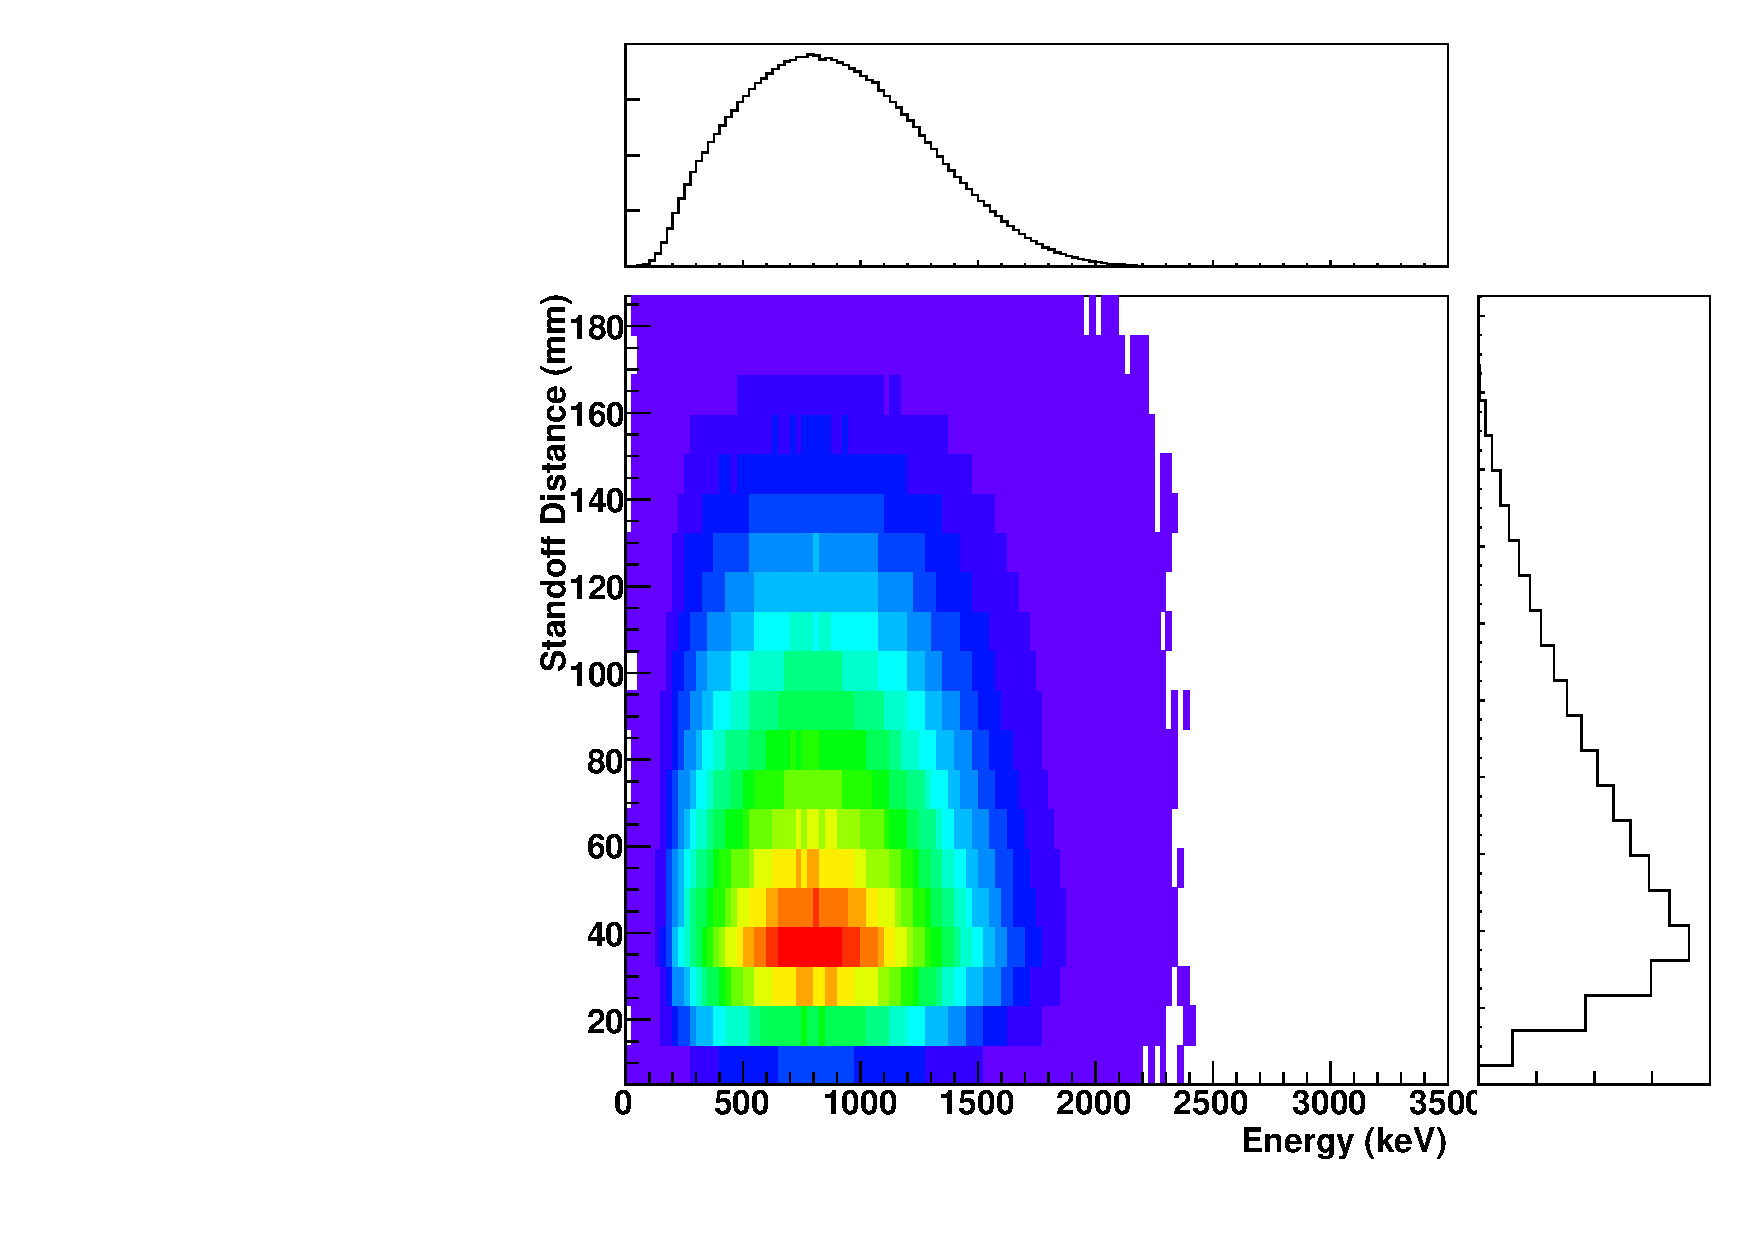
\includegraphics[width=\textwidth]{./plots/PDFs/analysis_pdf_bb2n_ss.pdf}
\end{subfigure}\hspace{0.1\textwidth}%
\begin{subfigure}[b]{0.35\textwidth}
	\centering
	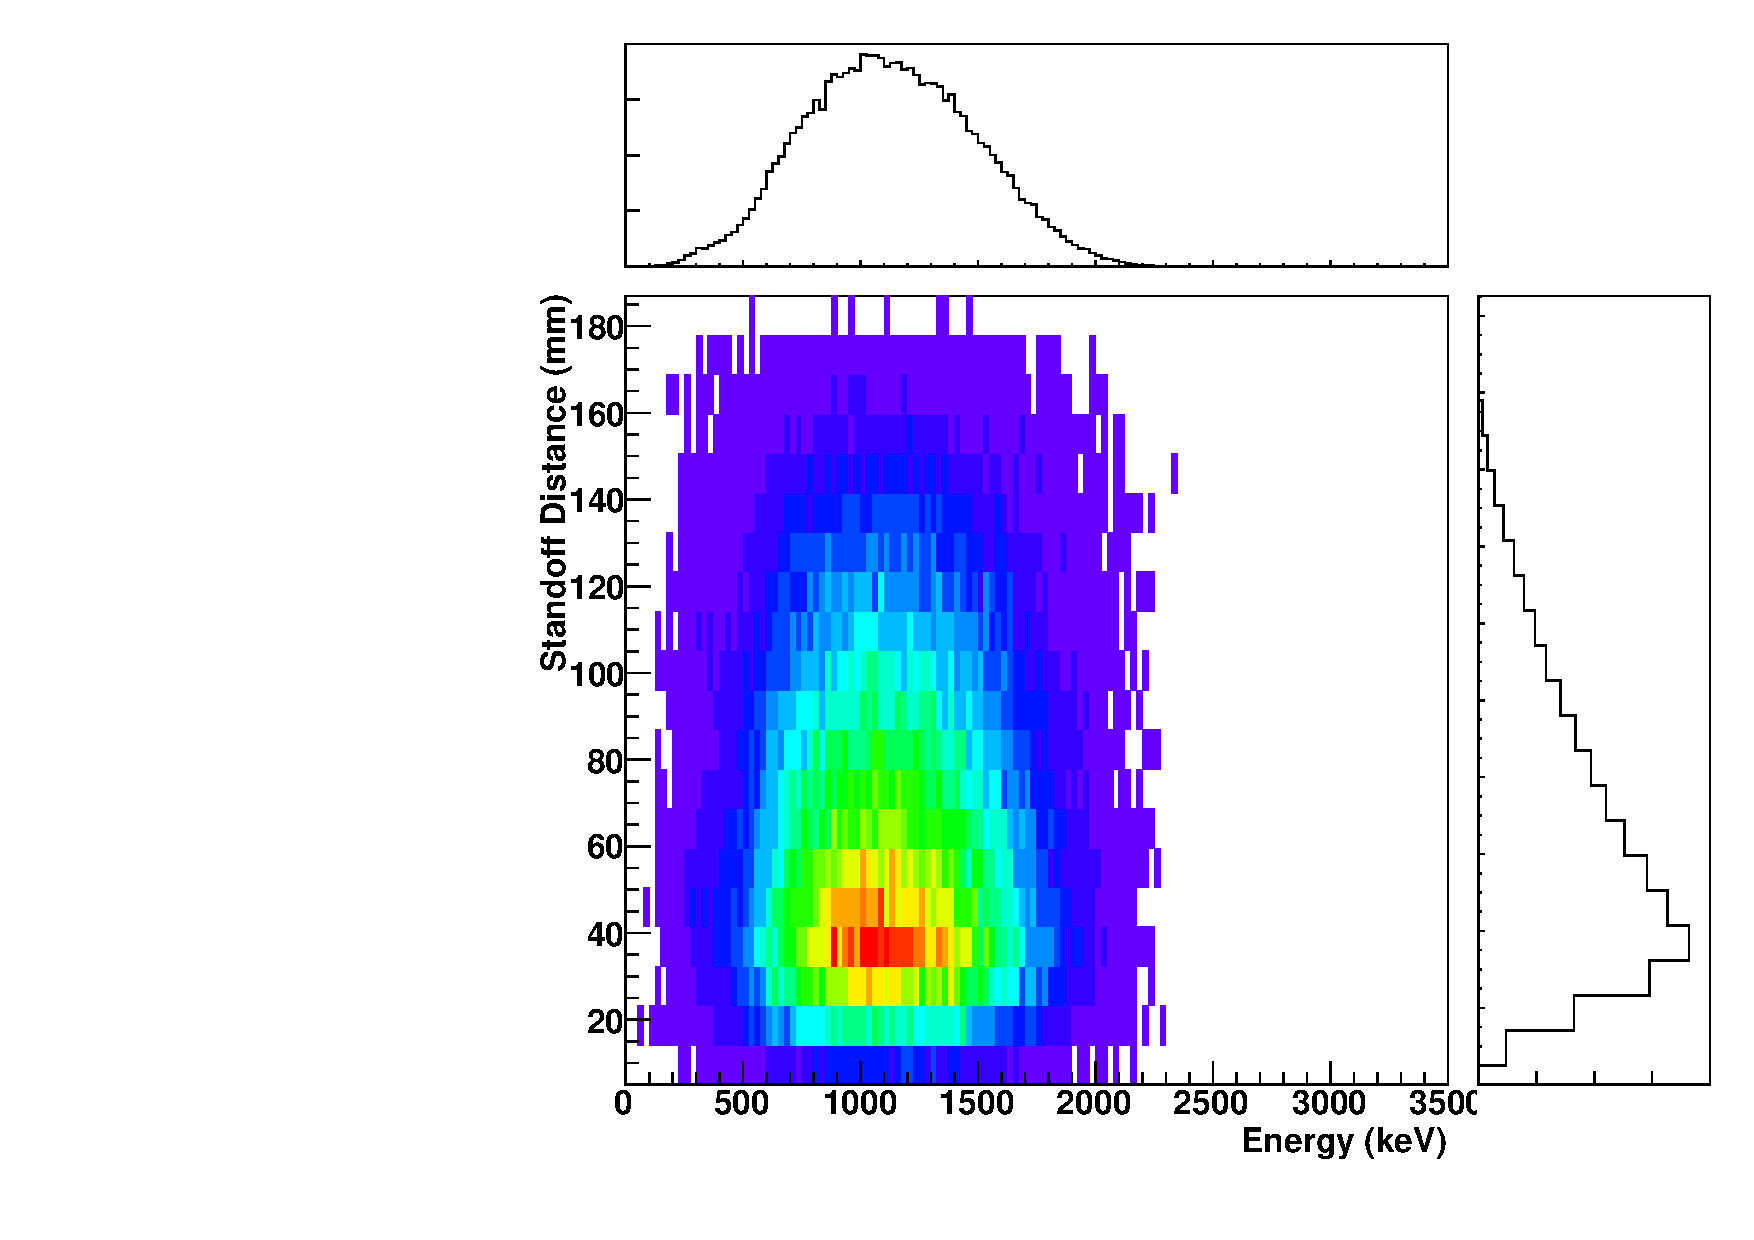
\includegraphics[width=1\textwidth]{./plots/PDFs/analysis_pdf_bb2n_ms.pdf}
	\end{subfigure}
\caption[PDF for \twonu{}]{The two dimensional PDFs for \twonu{}, with one-dimensional projections. Single site is shown on the left, and multiple site is shown on the right.}
\label{fig:analysis_pdf_bb2n}
\end{figure}

\begin{figure}[hp]
\centering
	\begin{subfigure}[b]{0.35\textwidth}
	\centering
	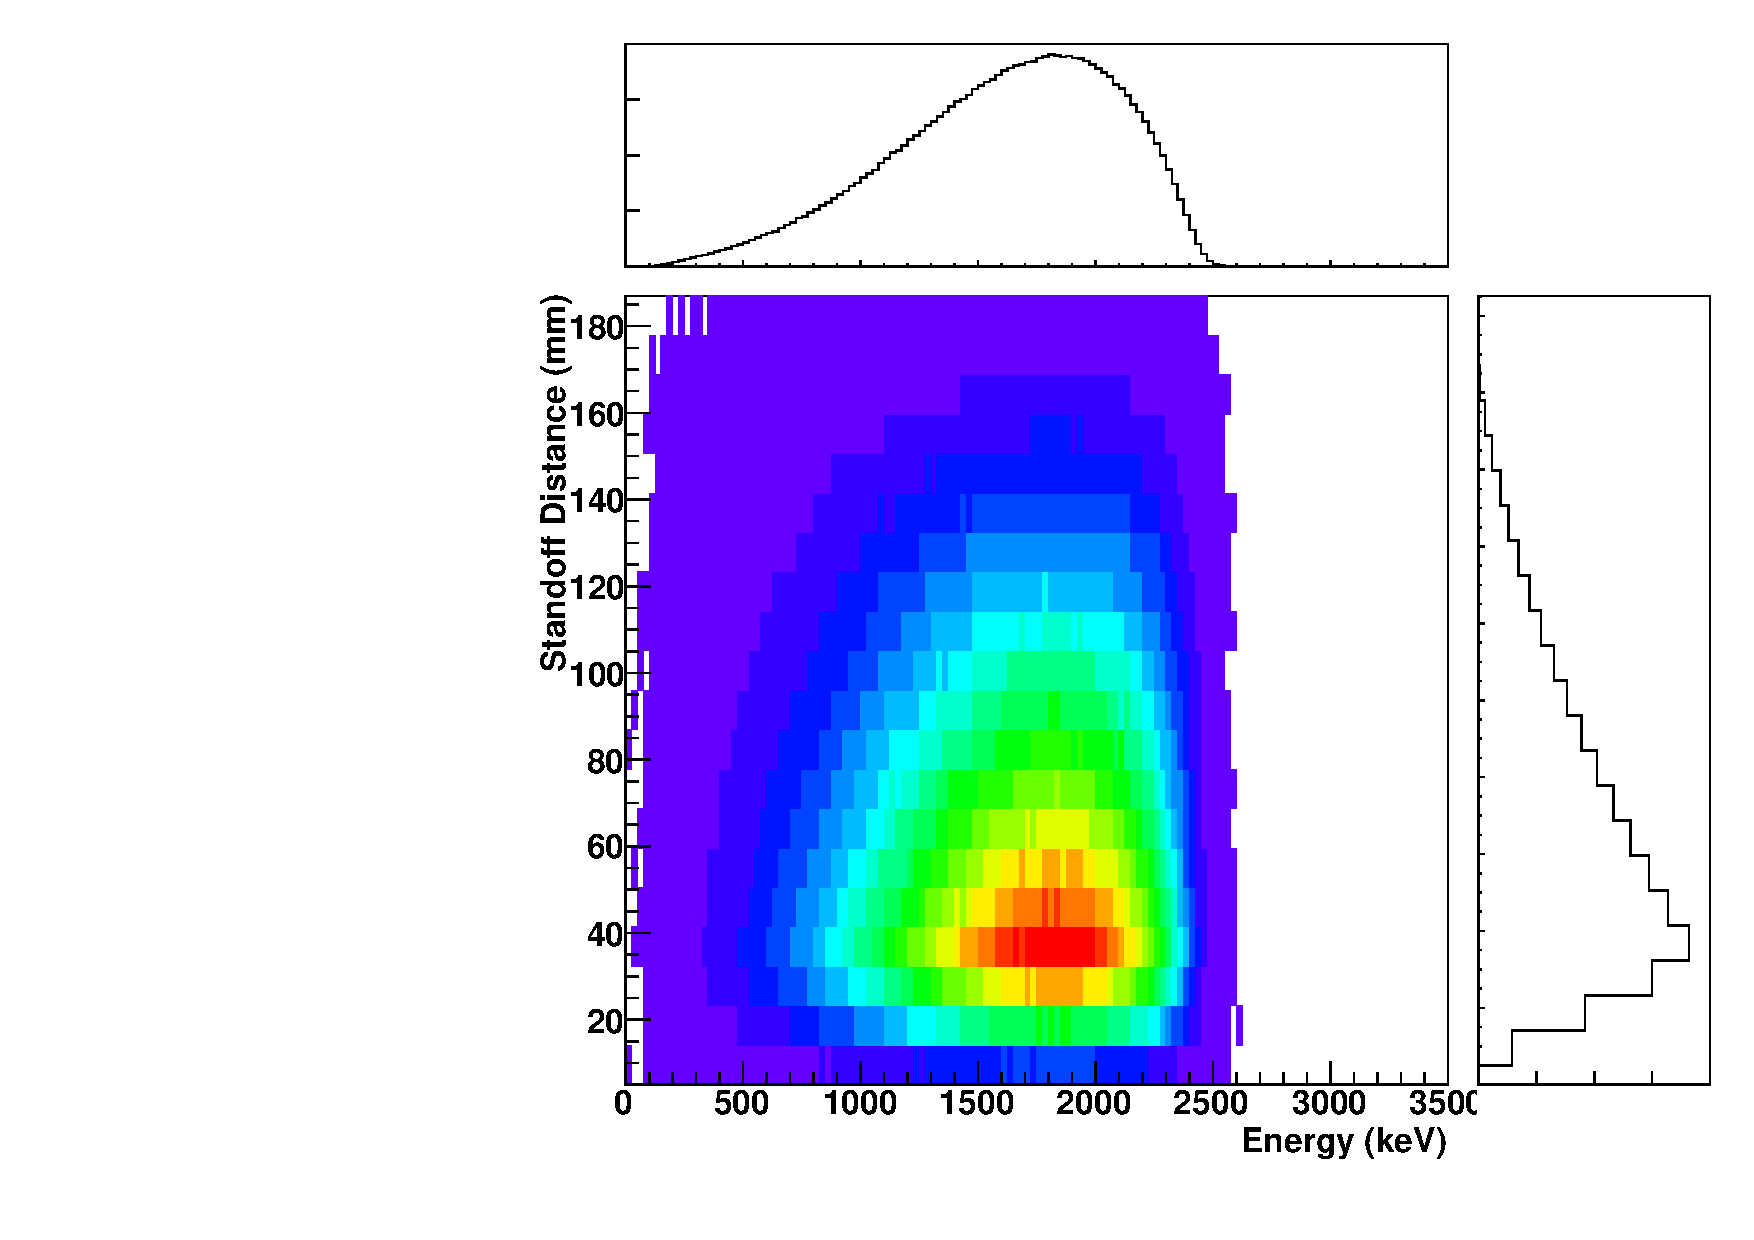
\includegraphics[width=\textwidth]{./plots/PDFs/analysis_pdf_bb0nX1_ss.pdf}
\end{subfigure}\hspace{0.1\textwidth}%
\begin{subfigure}[b]{0.35\textwidth}
	\centering
	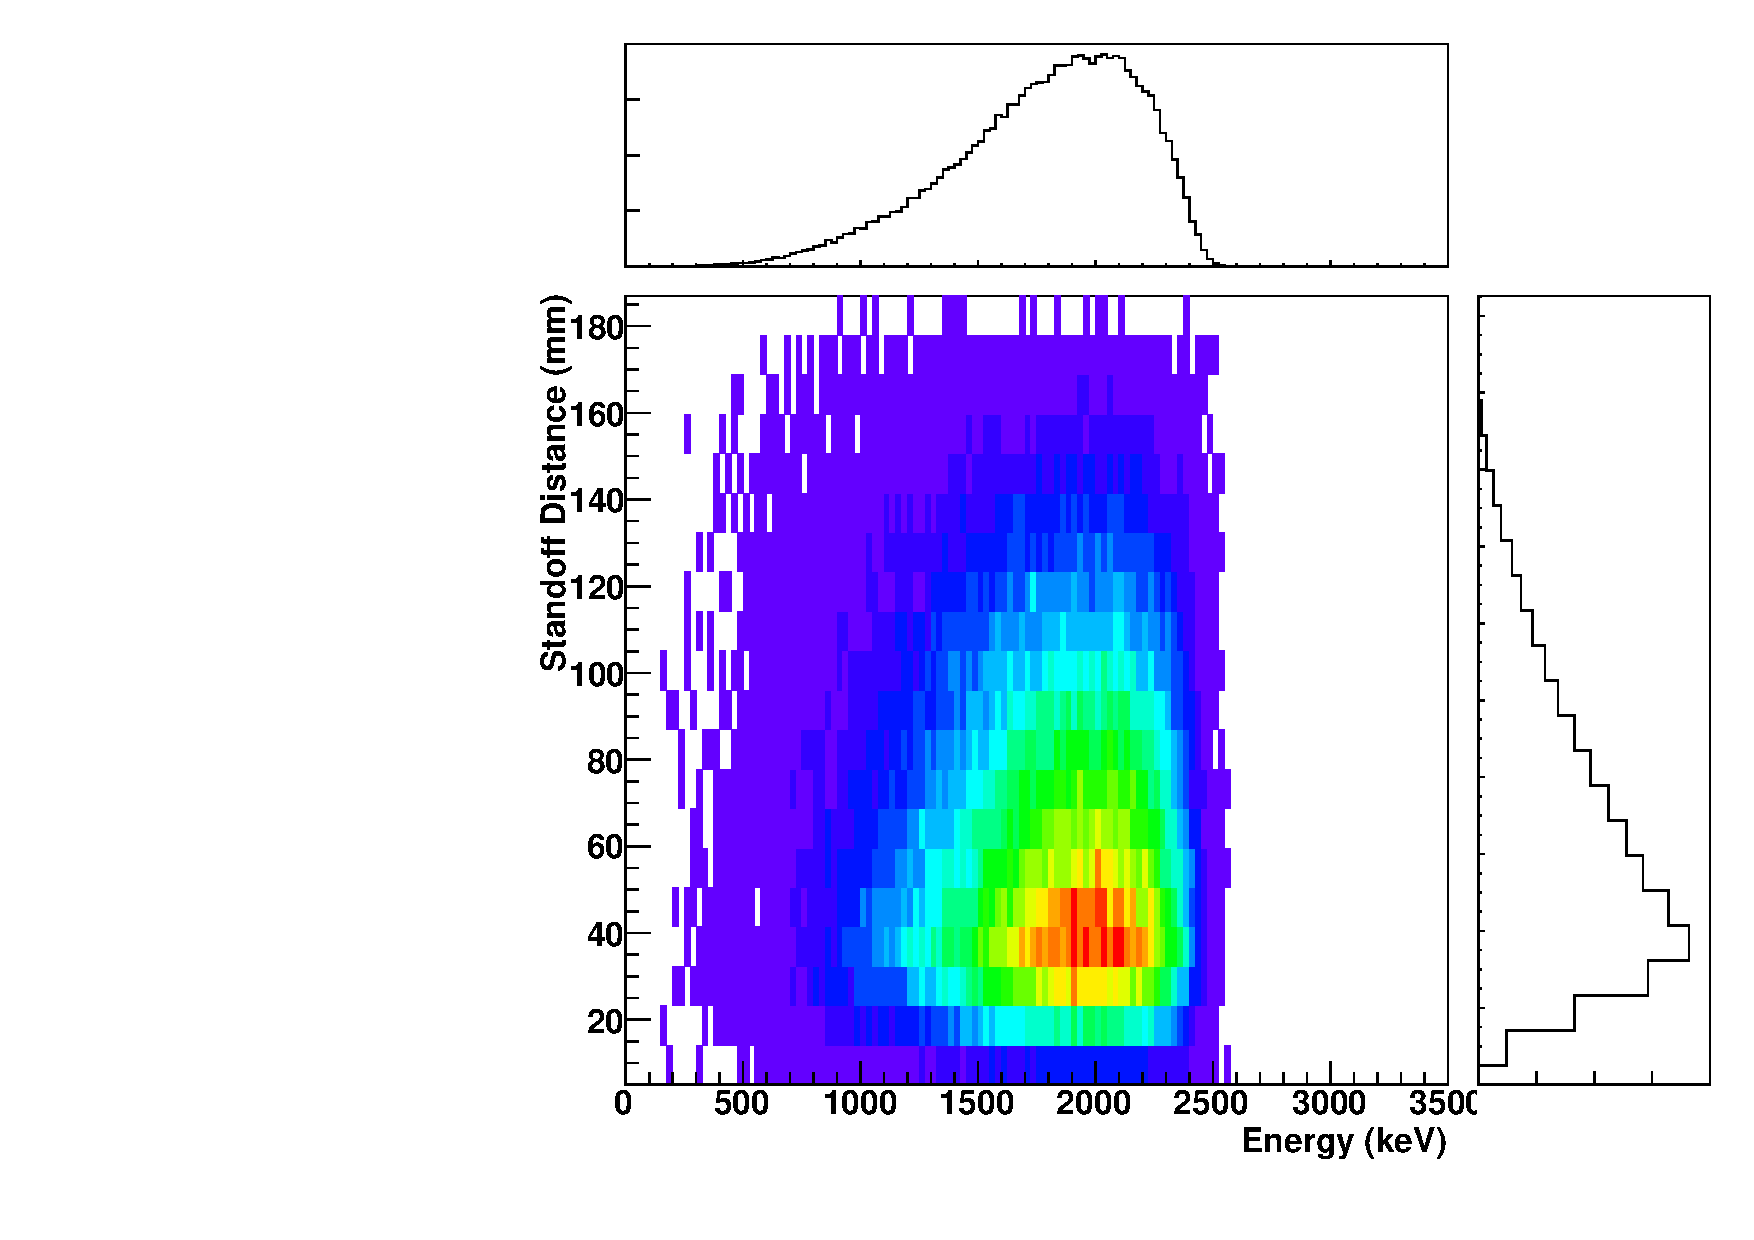
\includegraphics[width=1\textwidth]{./plots/PDFs/analysis_pdf_bb0nX1_ms.pdf}
	\end{subfigure}
\caption[PDF for \twonu{}]{The two dimensional PDFs for \(0\nu\beta\beta\chi^{0}\) with spectral index 1, with one-dimensional projections. Single site is shown on the left, and multiple site is shown on the right.}
\label{fig:analysis_pdf_bb0nX1}
\end{figure}

\begin{figure}[hp]
\centering
	\begin{subfigure}[b]{0.35\textwidth}
	\centering
	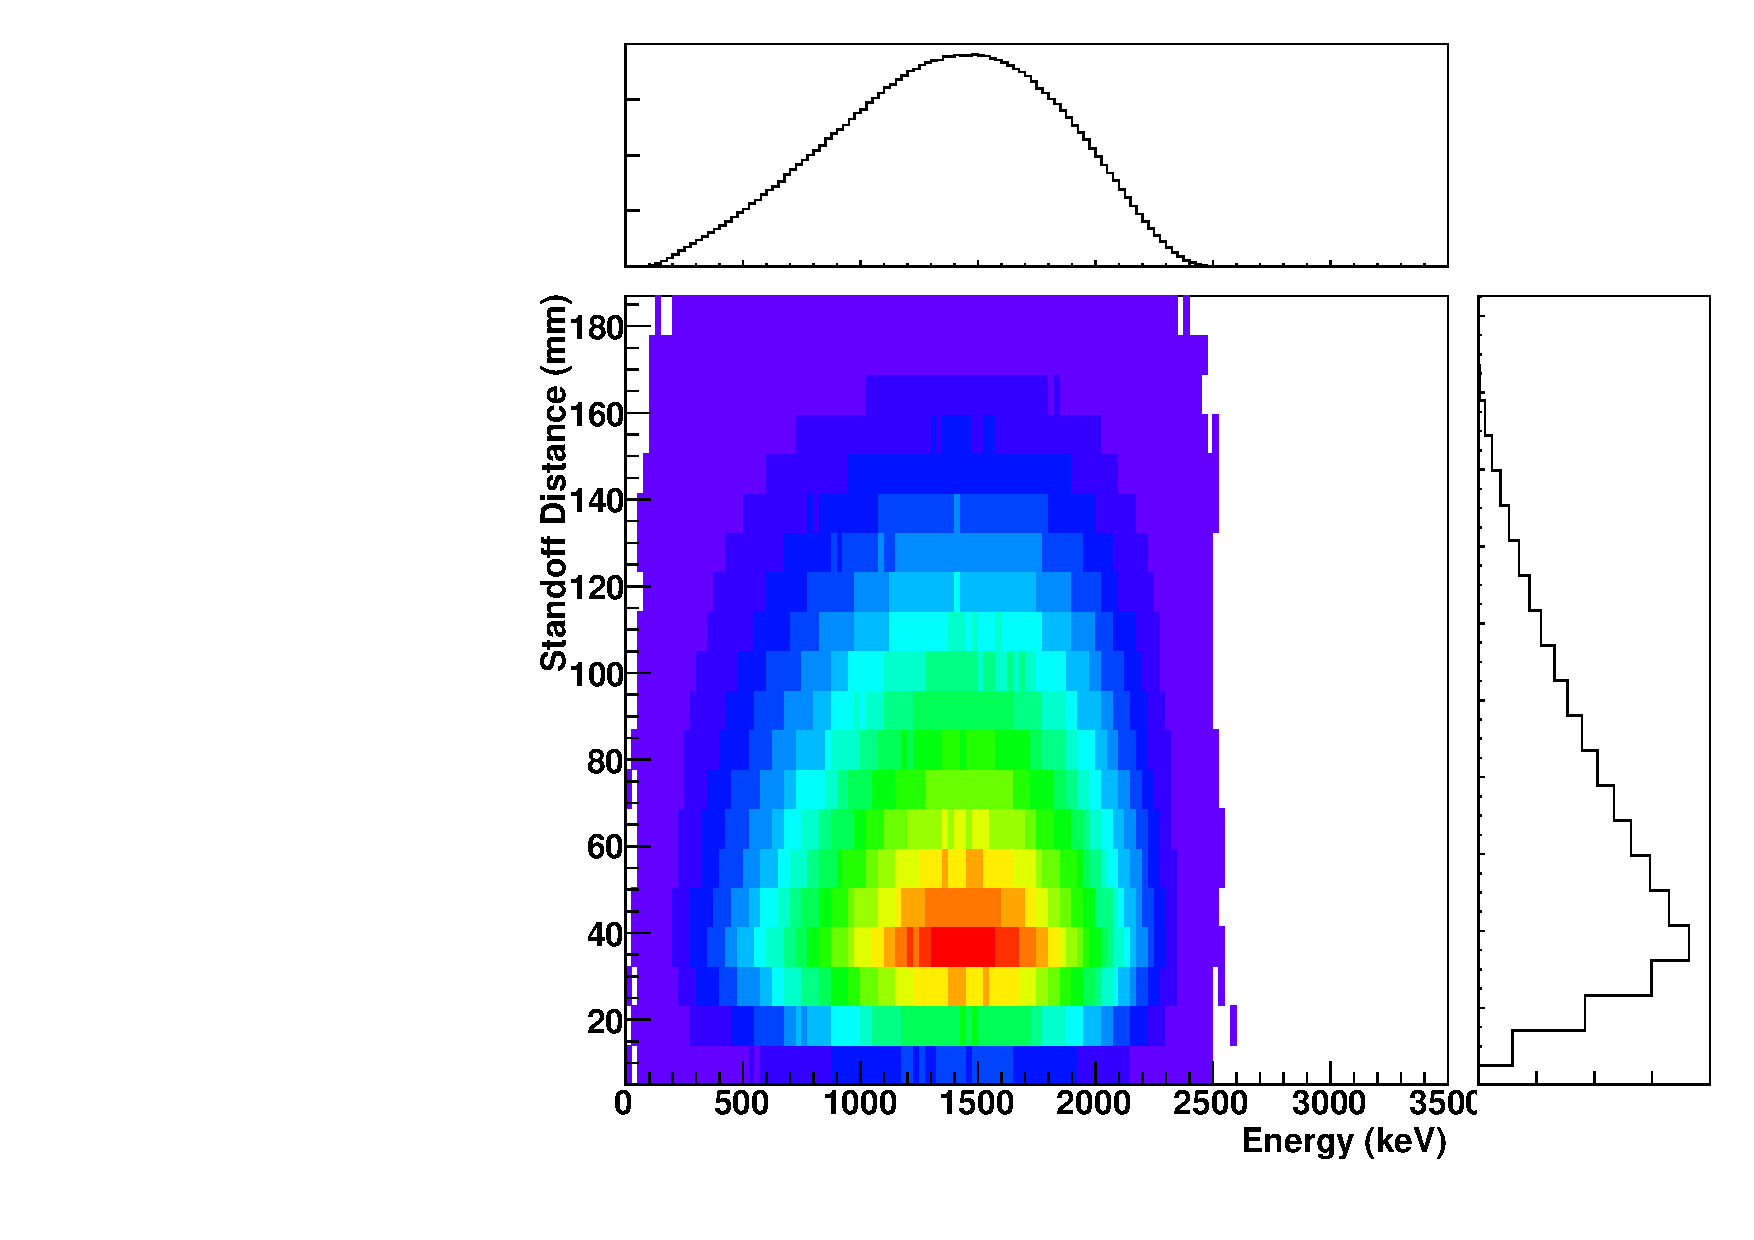
\includegraphics[width=\textwidth]{./plots/PDFs/analysis_pdf_bb0nX2_ss.pdf}
\end{subfigure}\hspace{0.1\textwidth}%
\begin{subfigure}[b]{0.35\textwidth}
	\centering
	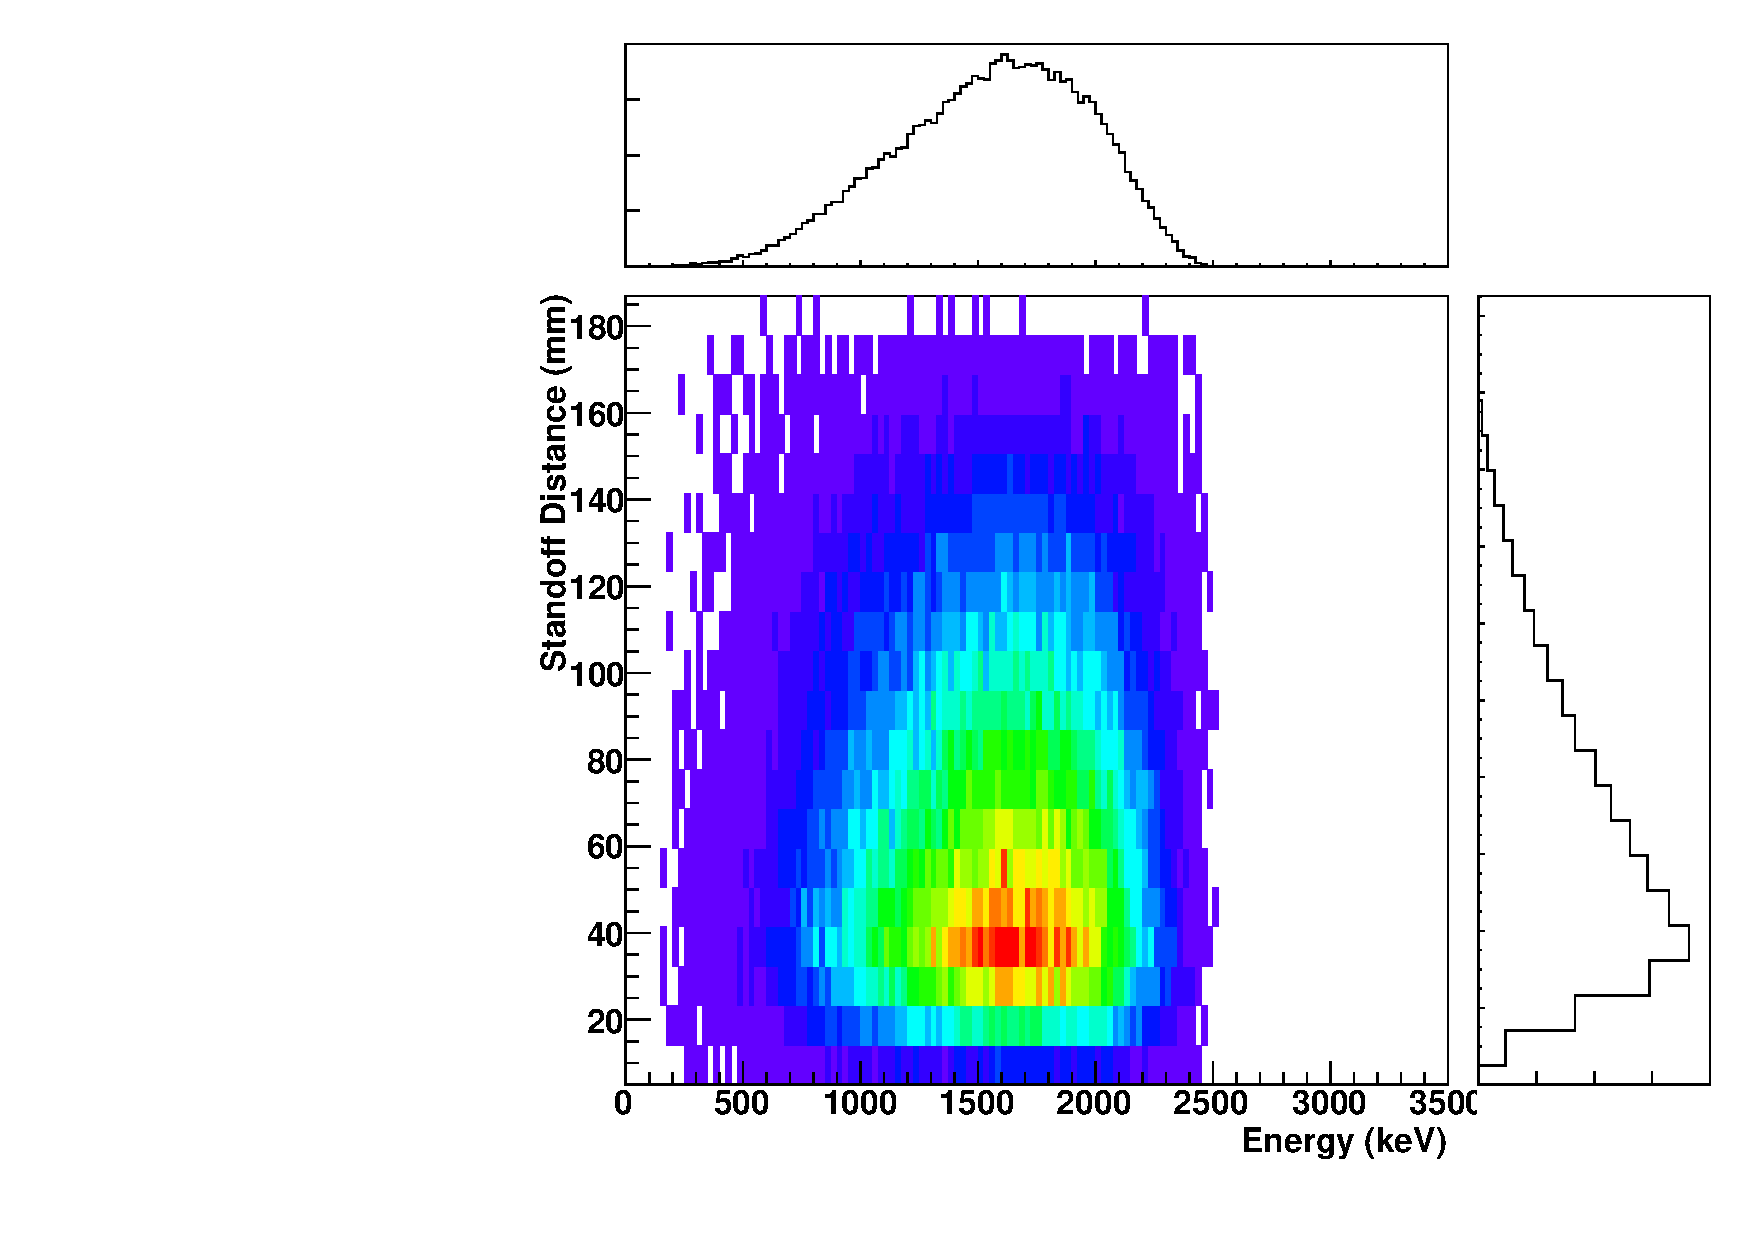
\includegraphics[width=1\textwidth]{./plots/PDFs/analysis_pdf_bb0nX2_ms.pdf}
	\end{subfigure}
\caption[PDF for \(0\nu\beta\beta\chi^{0}\)]{The two dimensional PDFs for \(0\nu\beta\beta\chi^{0}\) with spectral index 2, with one-dimensional projections. Single site is shown on the left, and multiple site is shown on the right.}
\label{fig:analysis_pdf_bb0nX2}
\end{figure}

\begin{figure}[hp]
\centering
	\begin{subfigure}[b]{0.35\textwidth}
	\centering
	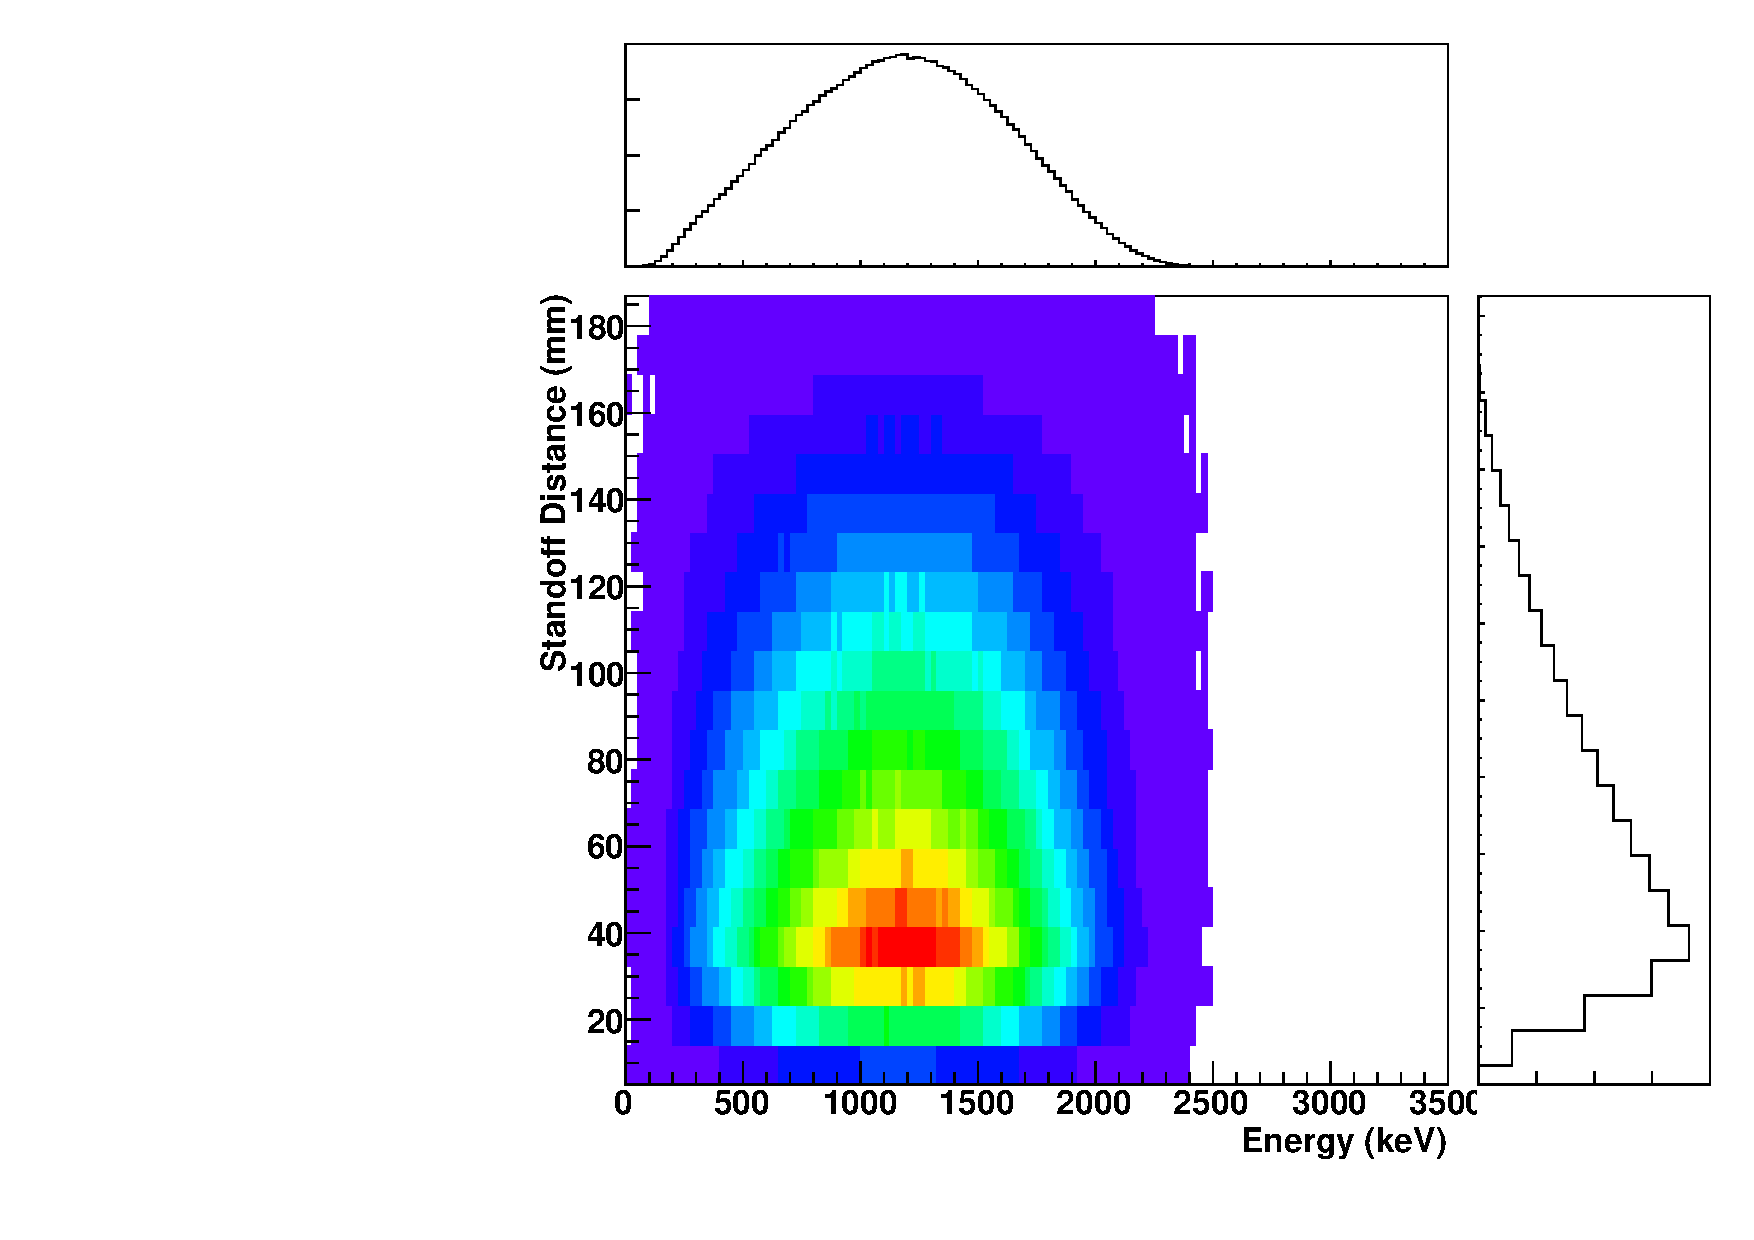
\includegraphics[width=\textwidth]{./plots/PDFs/analysis_pdf_bb0nX3_ss.pdf}
\end{subfigure}\hspace{0.1\textwidth}%
\begin{subfigure}[b]{0.35\textwidth}
	\centering
	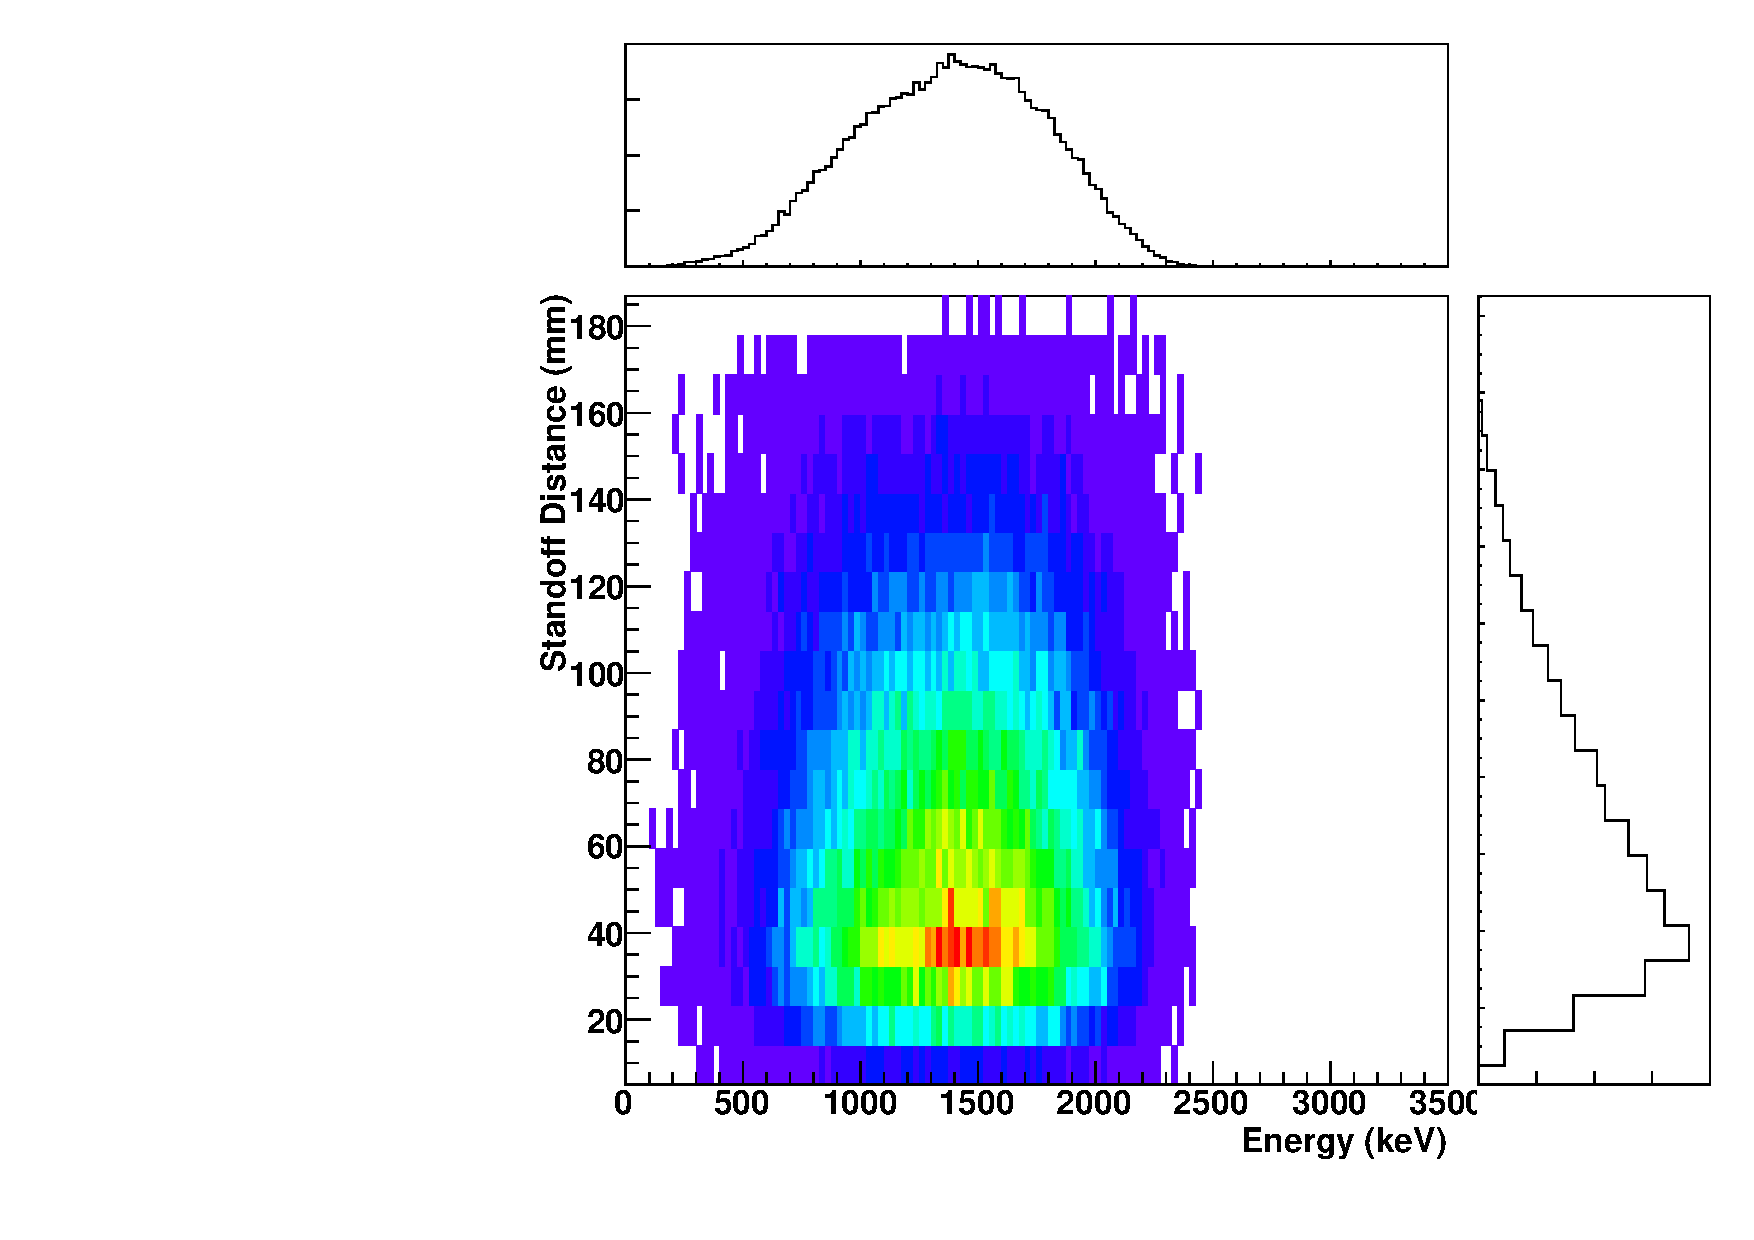
\includegraphics[width=1\textwidth]{./plots/PDFs/analysis_pdf_bb0nX3_ms.pdf}
	\end{subfigure}
\caption[PDF for  \(0\nu\beta\beta\chi^{0}(\chi^{0})\)]{The two dimensional PDFs for \(0\nu\beta\beta\chi^{0}(\chi^{0})\) with spectral index 3, with one-dimensional projections. Single site is shown on the left, and multiple site is shown on the right.}
\label{fig:analysis_pdf_bb0nX3}
\end{figure}

\begin{figure}[hp]
\centering
	\begin{subfigure}[b]{0.35\textwidth}
	\centering
	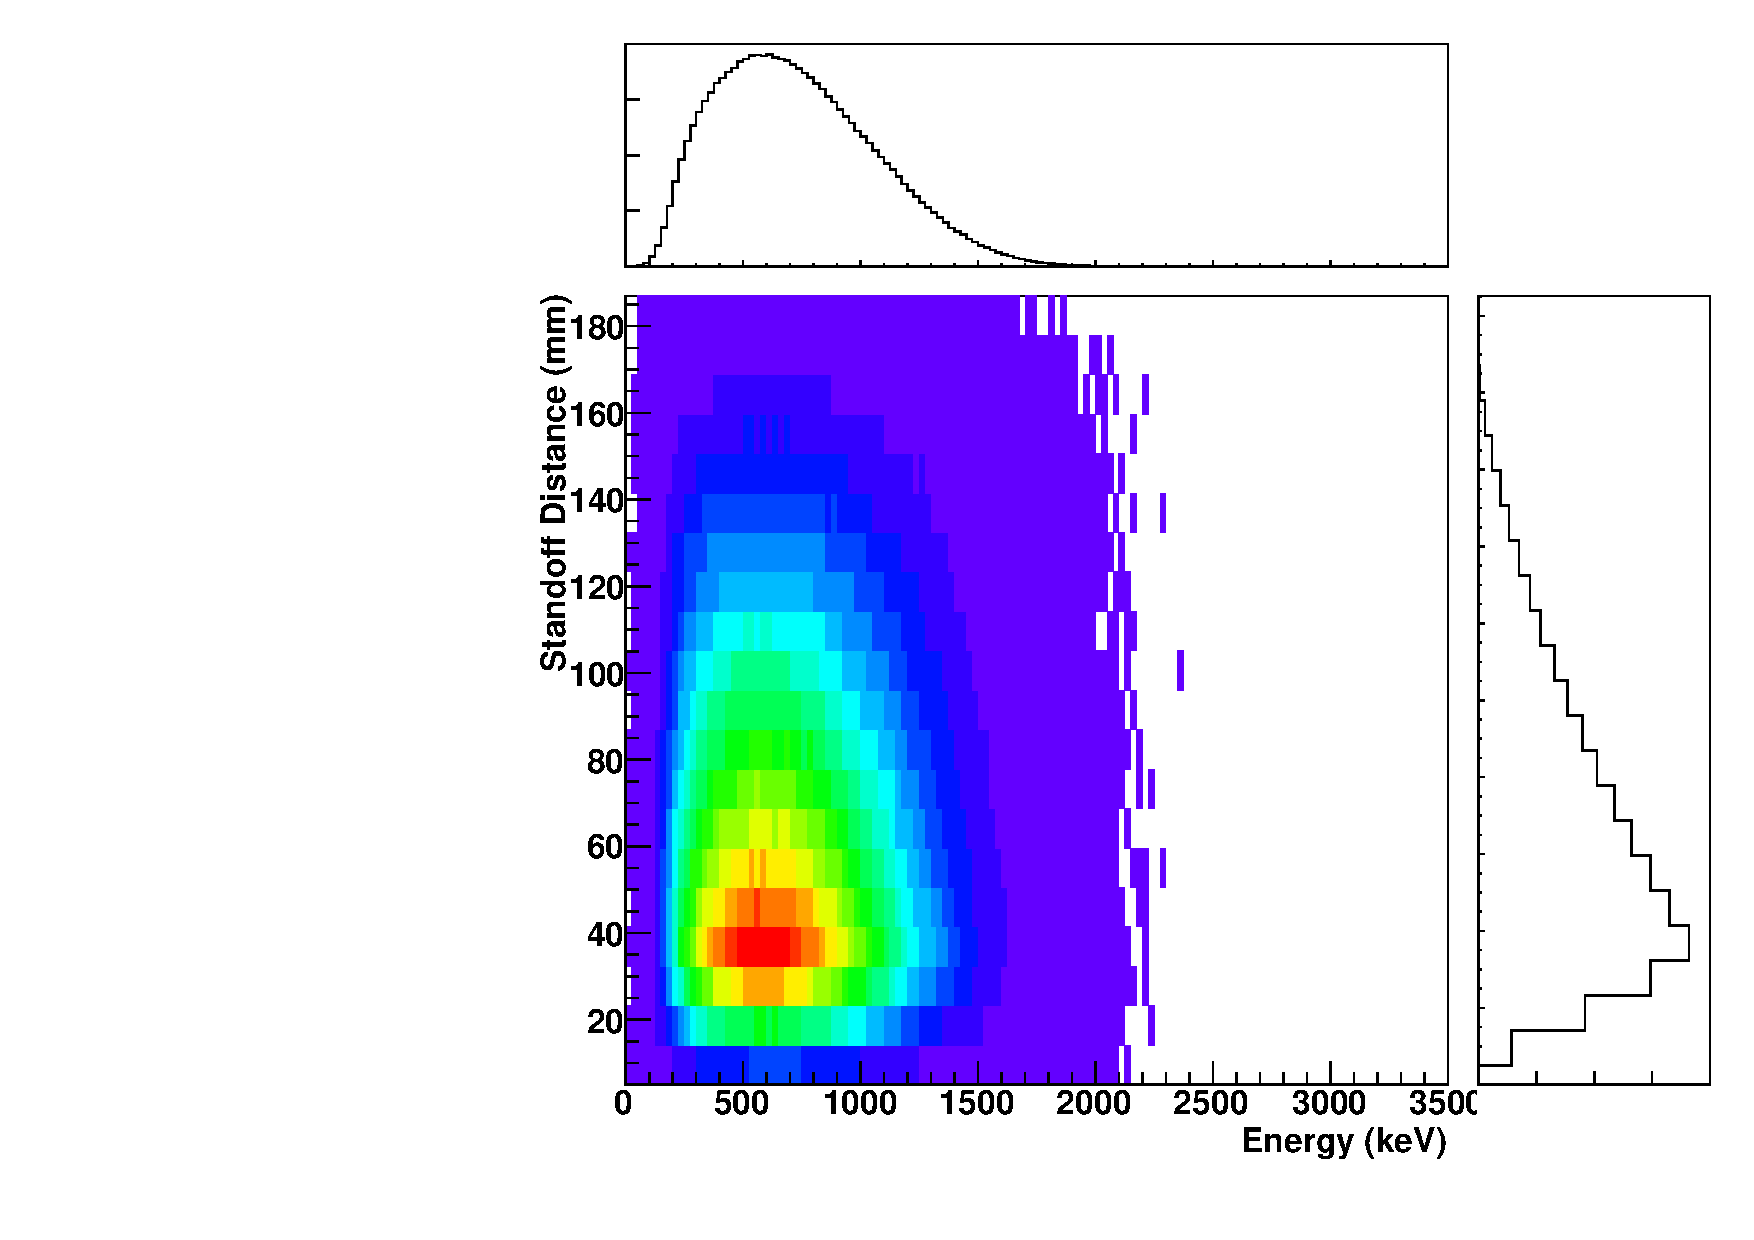
\includegraphics[width=\textwidth]{./plots/PDFs/analysis_pdf_bb0nX7_ss.pdf}
\end{subfigure}\hspace{0.1\textwidth}%
\begin{subfigure}[b]{0.35\textwidth}
	\centering
	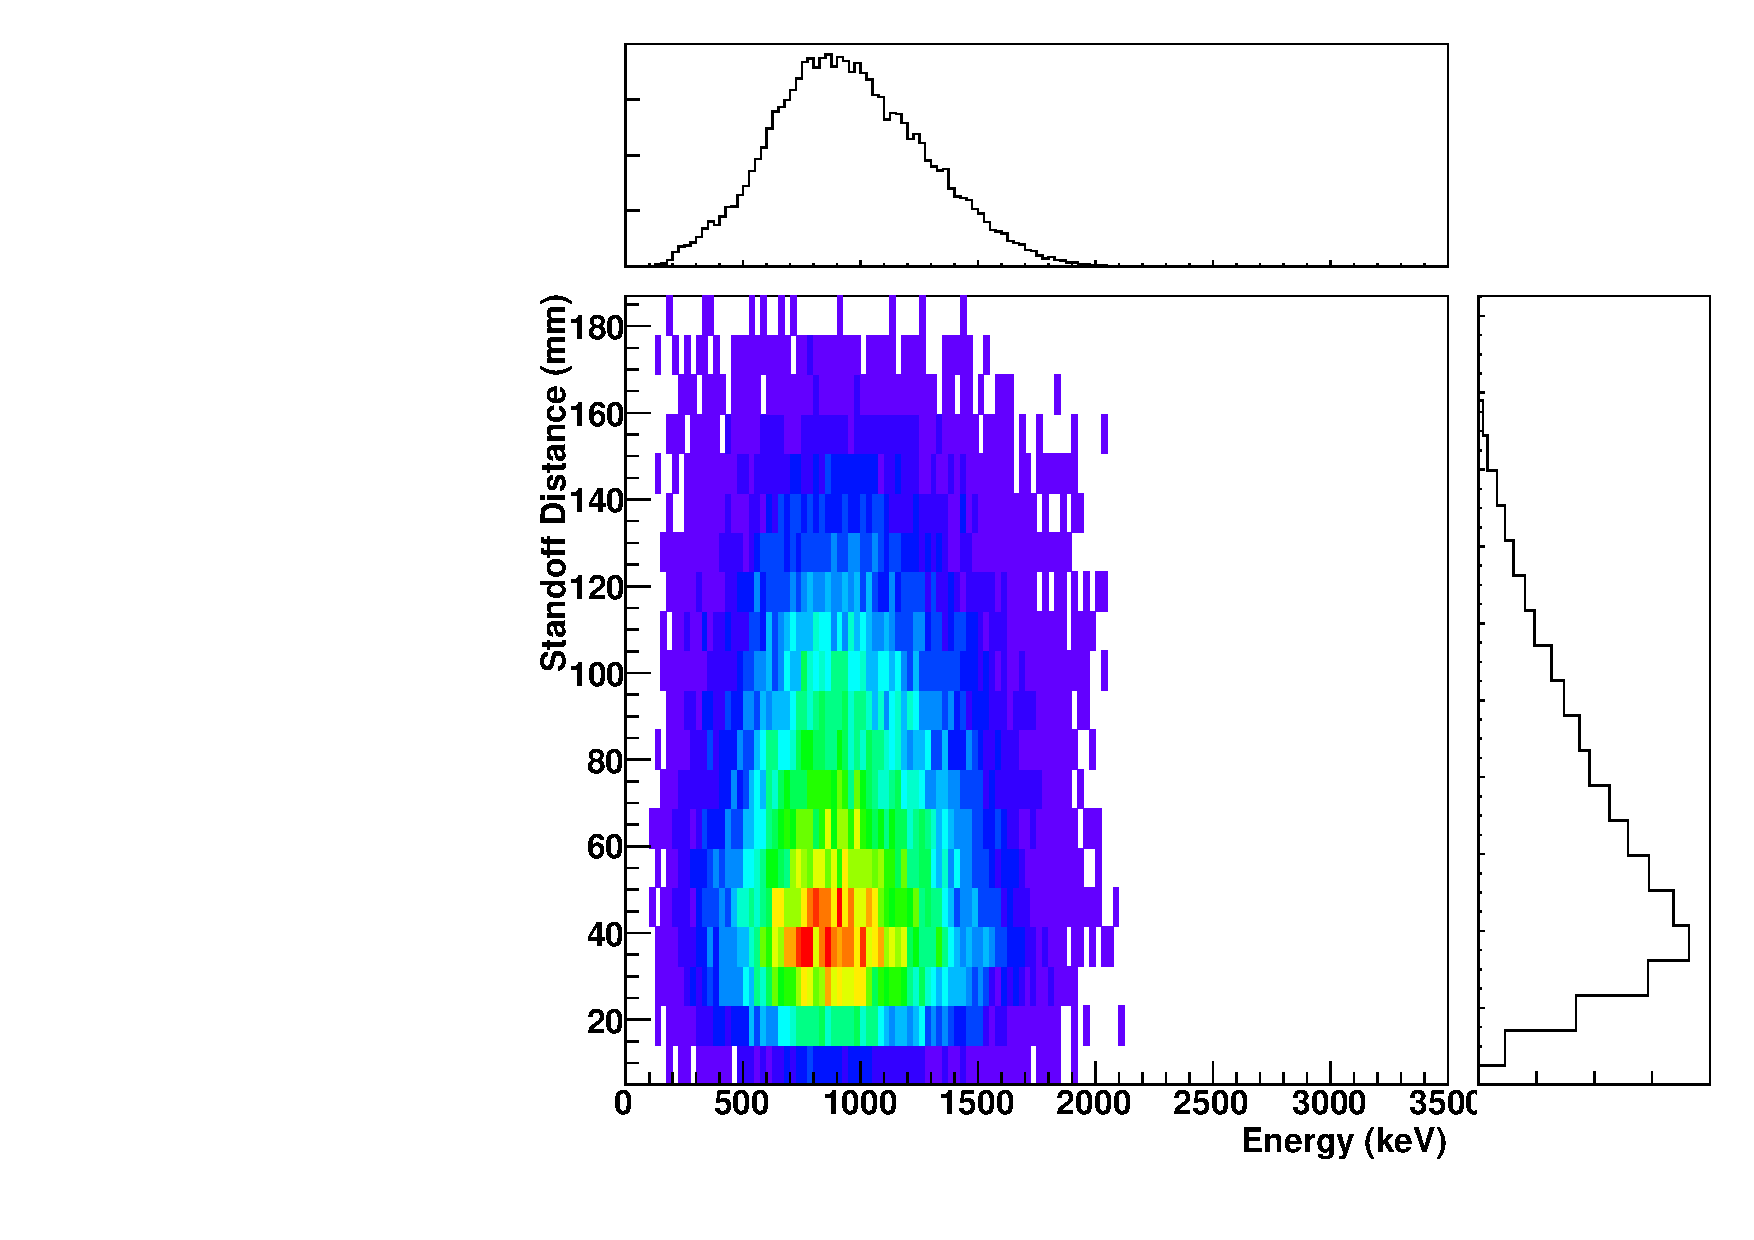
\includegraphics[width=1\textwidth]{./plots/PDFs/analysis_pdf_bb0nX7_ms.pdf}
	\end{subfigure}
\caption[PDF for \(0\nu\beta\beta\chi^{0}\chi^{0}\)]{The two dimensional PDFs for \(0\nu\beta\beta\chi^{0}\chi^{0}\) with spectral index 7, with one-dimensional projections. Single site is shown on the left, and multiple site is shown on the right.}
\label{fig:analysis_pdf_bb0nX7}
\end{figure}

\begin{figure}[hp]
\centering
	\begin{subfigure}[b]{0.35\textwidth}
	\centering
	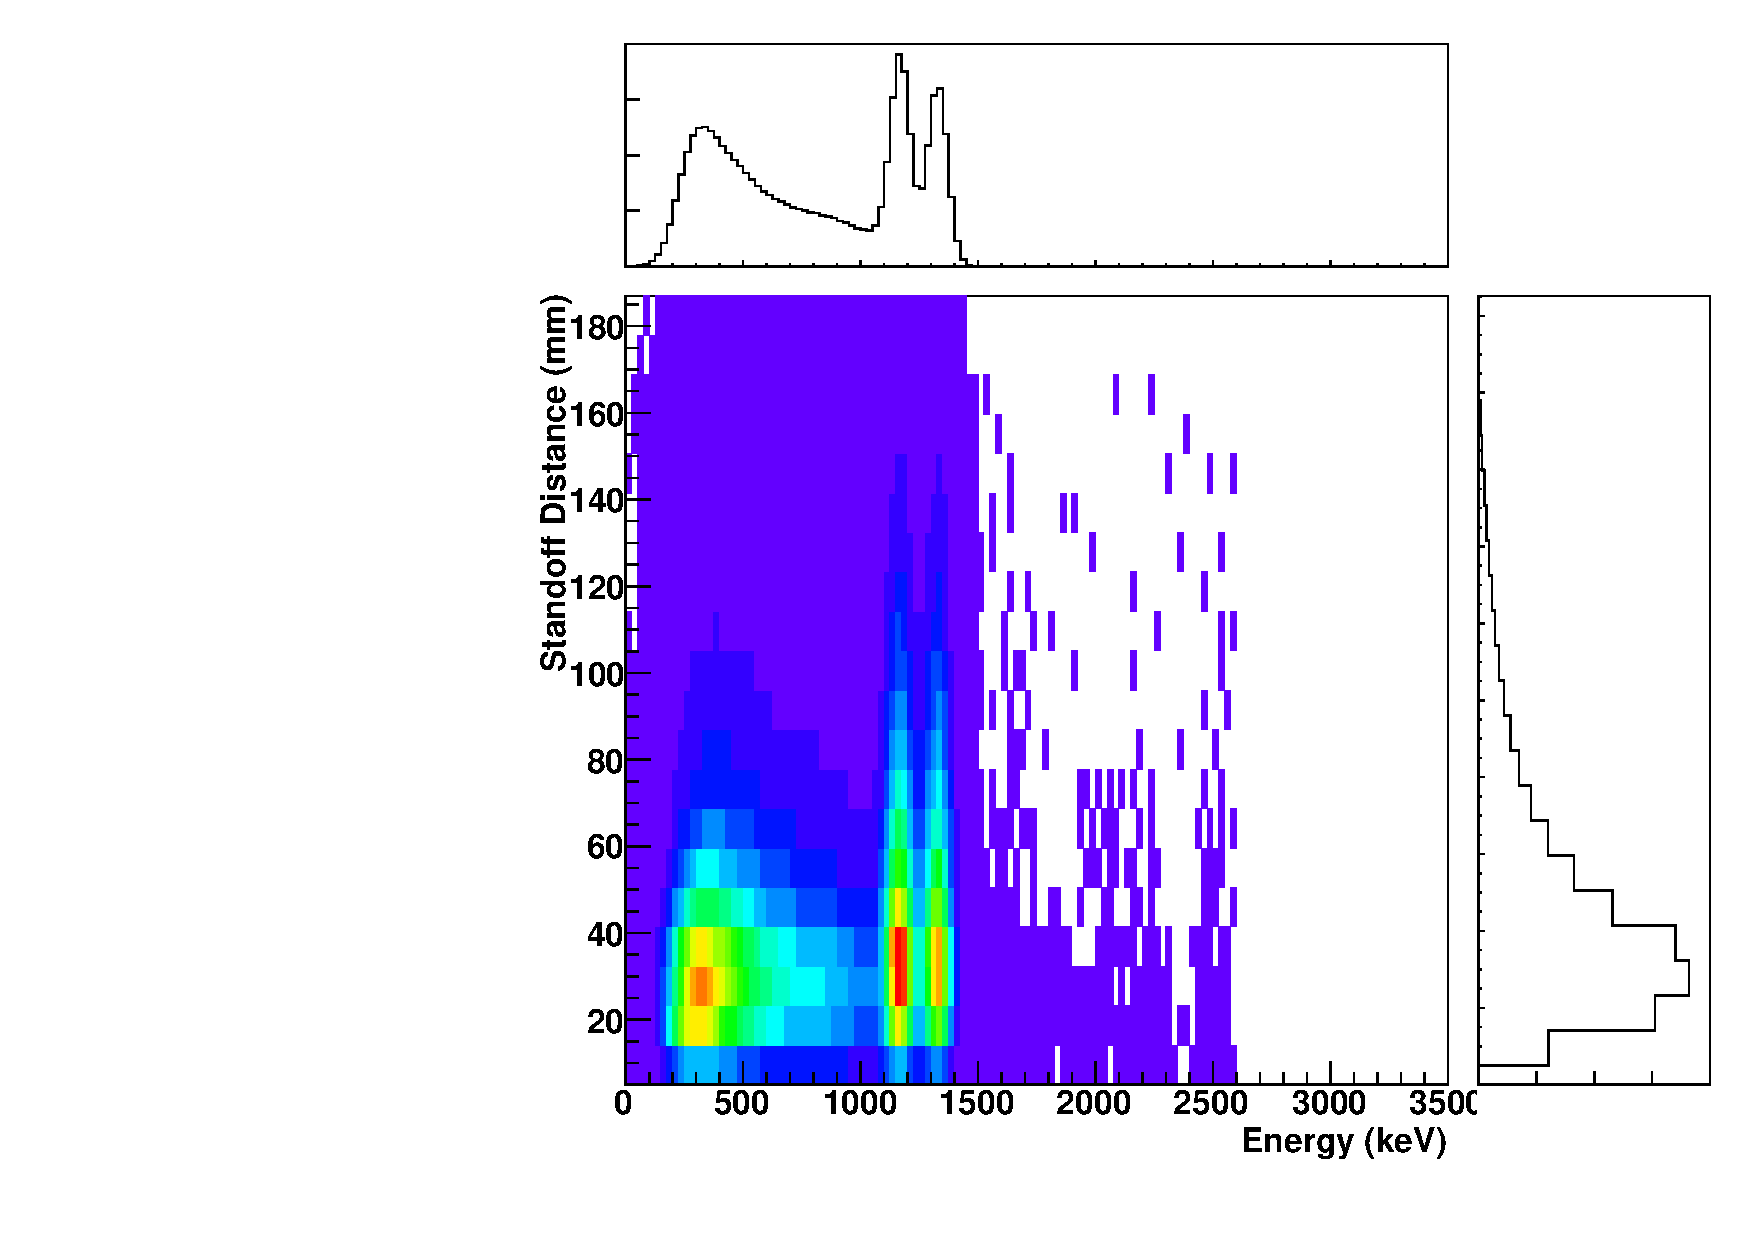
\includegraphics[width=\textwidth]{./plots/PDFs/analysis_pdf_AllVessel_Co60_ss.pdf}
\end{subfigure}\hspace{0.1\textwidth}%
\begin{subfigure}[b]{0.35\textwidth}
	\centering
	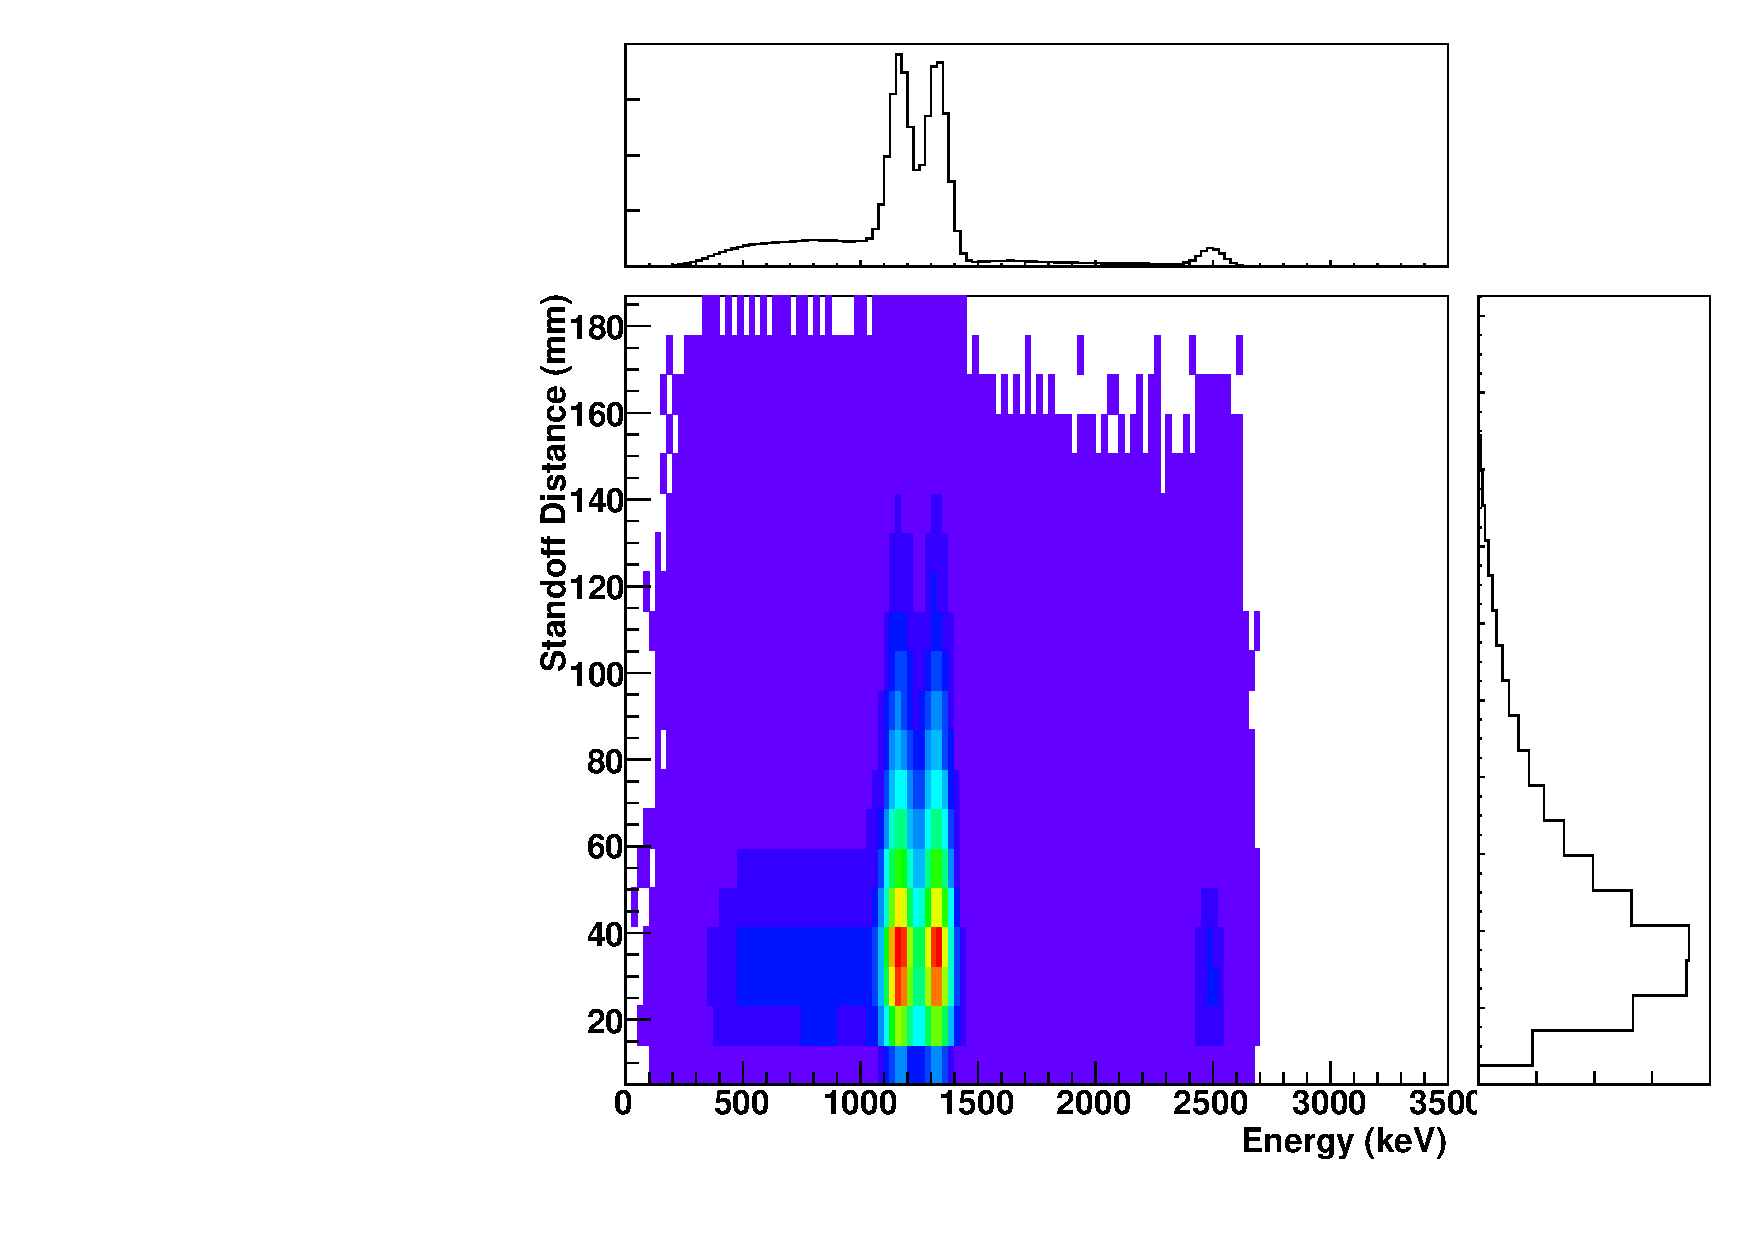
\includegraphics[width=1\textwidth]{./plots/PDFs/analysis_pdf_AllVessel_Co60_ms.pdf}
	\end{subfigure}
\caption[PDF for \isotope{60}{Co} in the TPC vessel]{The two dimensional PDFs for \isotope{60}{Co} in the copper vessel, with one-dimensional projections. Single site is shown on the left, and multiple site is shown on the right.}
\label{fig:analysis_pdf_AllVessel_Co60}
\end{figure}

\begin{figure}[hp]
\centering
	\begin{subfigure}[b]{0.35\textwidth}
	\centering
	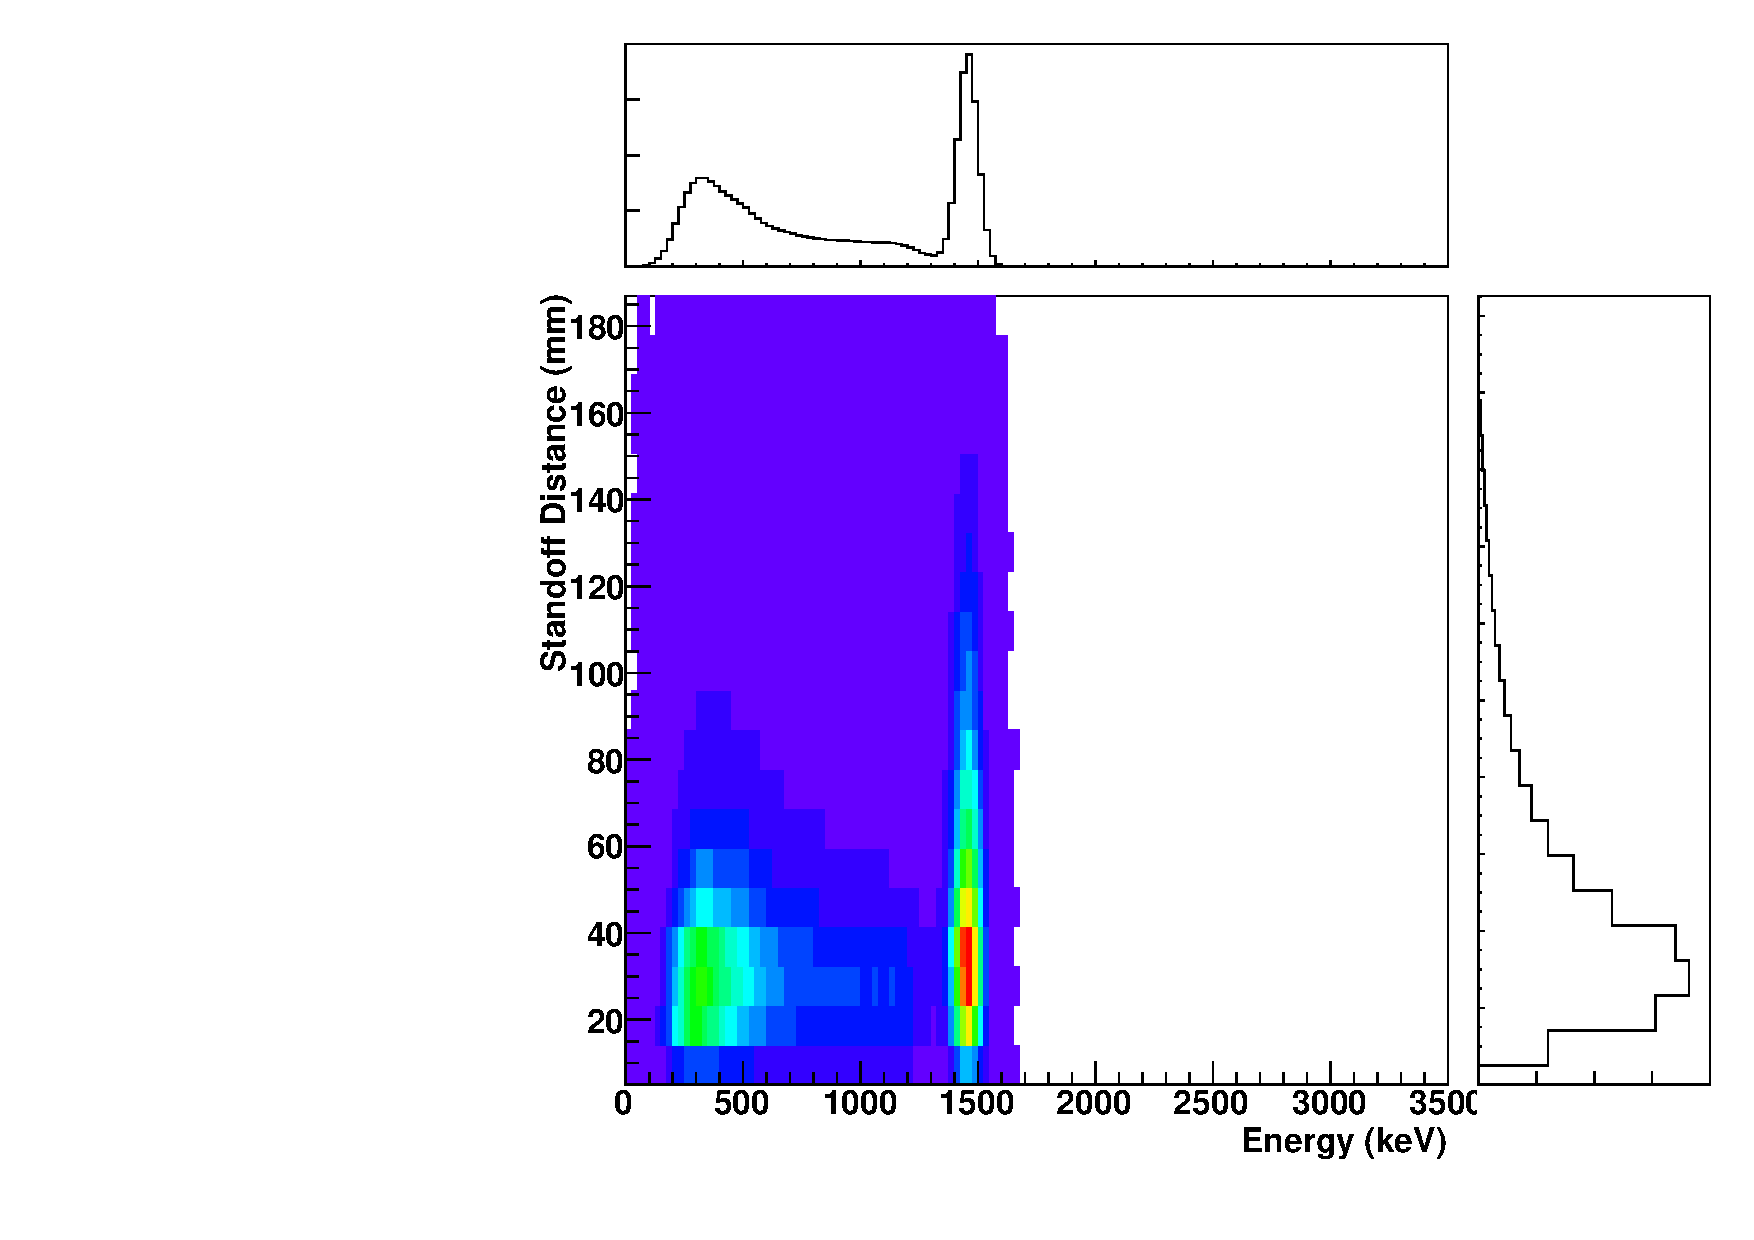
\includegraphics[width=\textwidth]{./plots/PDFs/analysis_pdf_AllVessel_K40_ss.pdf}
\end{subfigure}\hspace{0.1\textwidth}%
\begin{subfigure}[b]{0.35\textwidth}
	\centering
	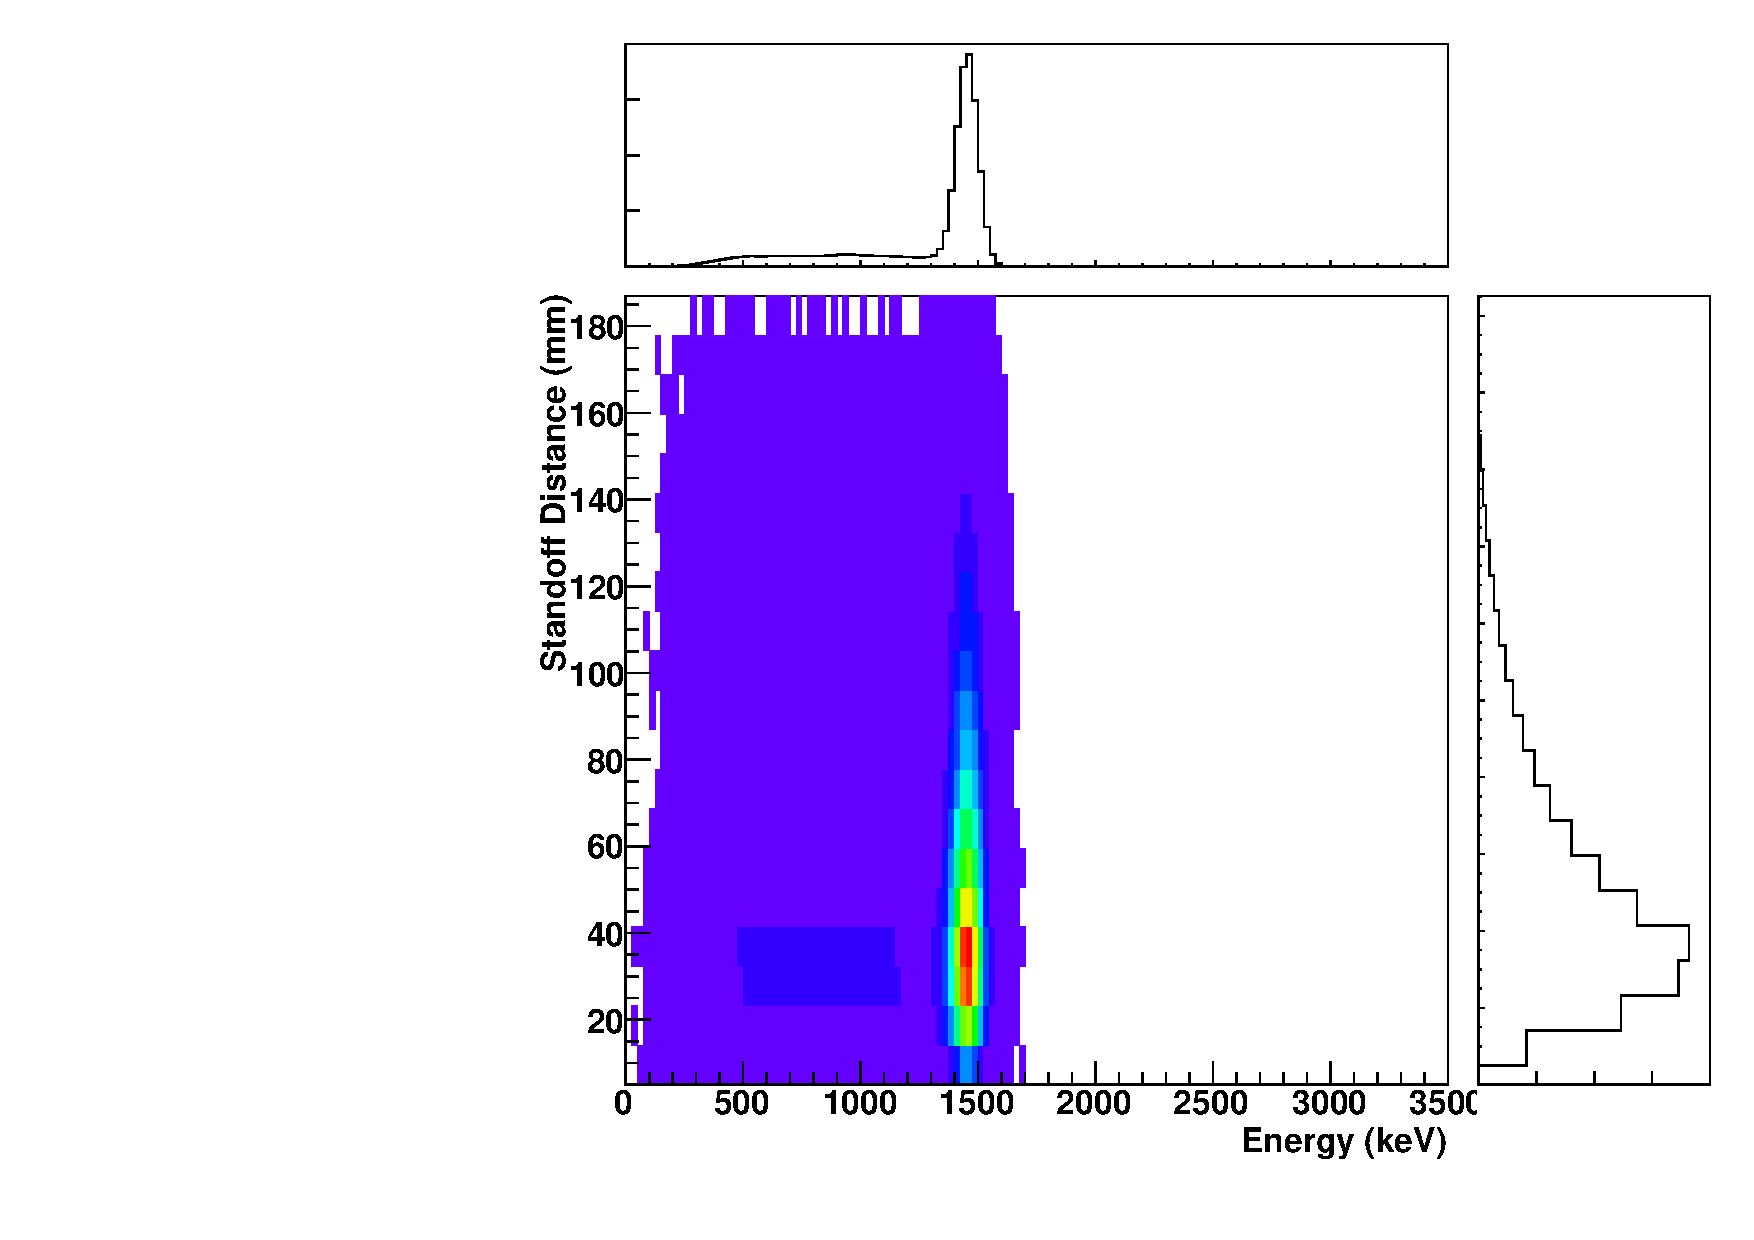
\includegraphics[width=1\textwidth]{./plots/PDFs/analysis_pdf_AllVessel_K40_ms.pdf}
	\end{subfigure}
\caption[PDF for \isotope{40}{K} in the TPC vessel]{The two dimensional PDFs for \isotope{40}{K} in the copper vessel, with one-dimensional projections. Single site is shown on the left, and multiple site is shown on the right.}
\label{fig:analysis_pdf_AllVessel_K40}
\end{figure}

\begin{figure}[hp]
\centering
	\begin{subfigure}[b]{0.35\textwidth}
	\centering
	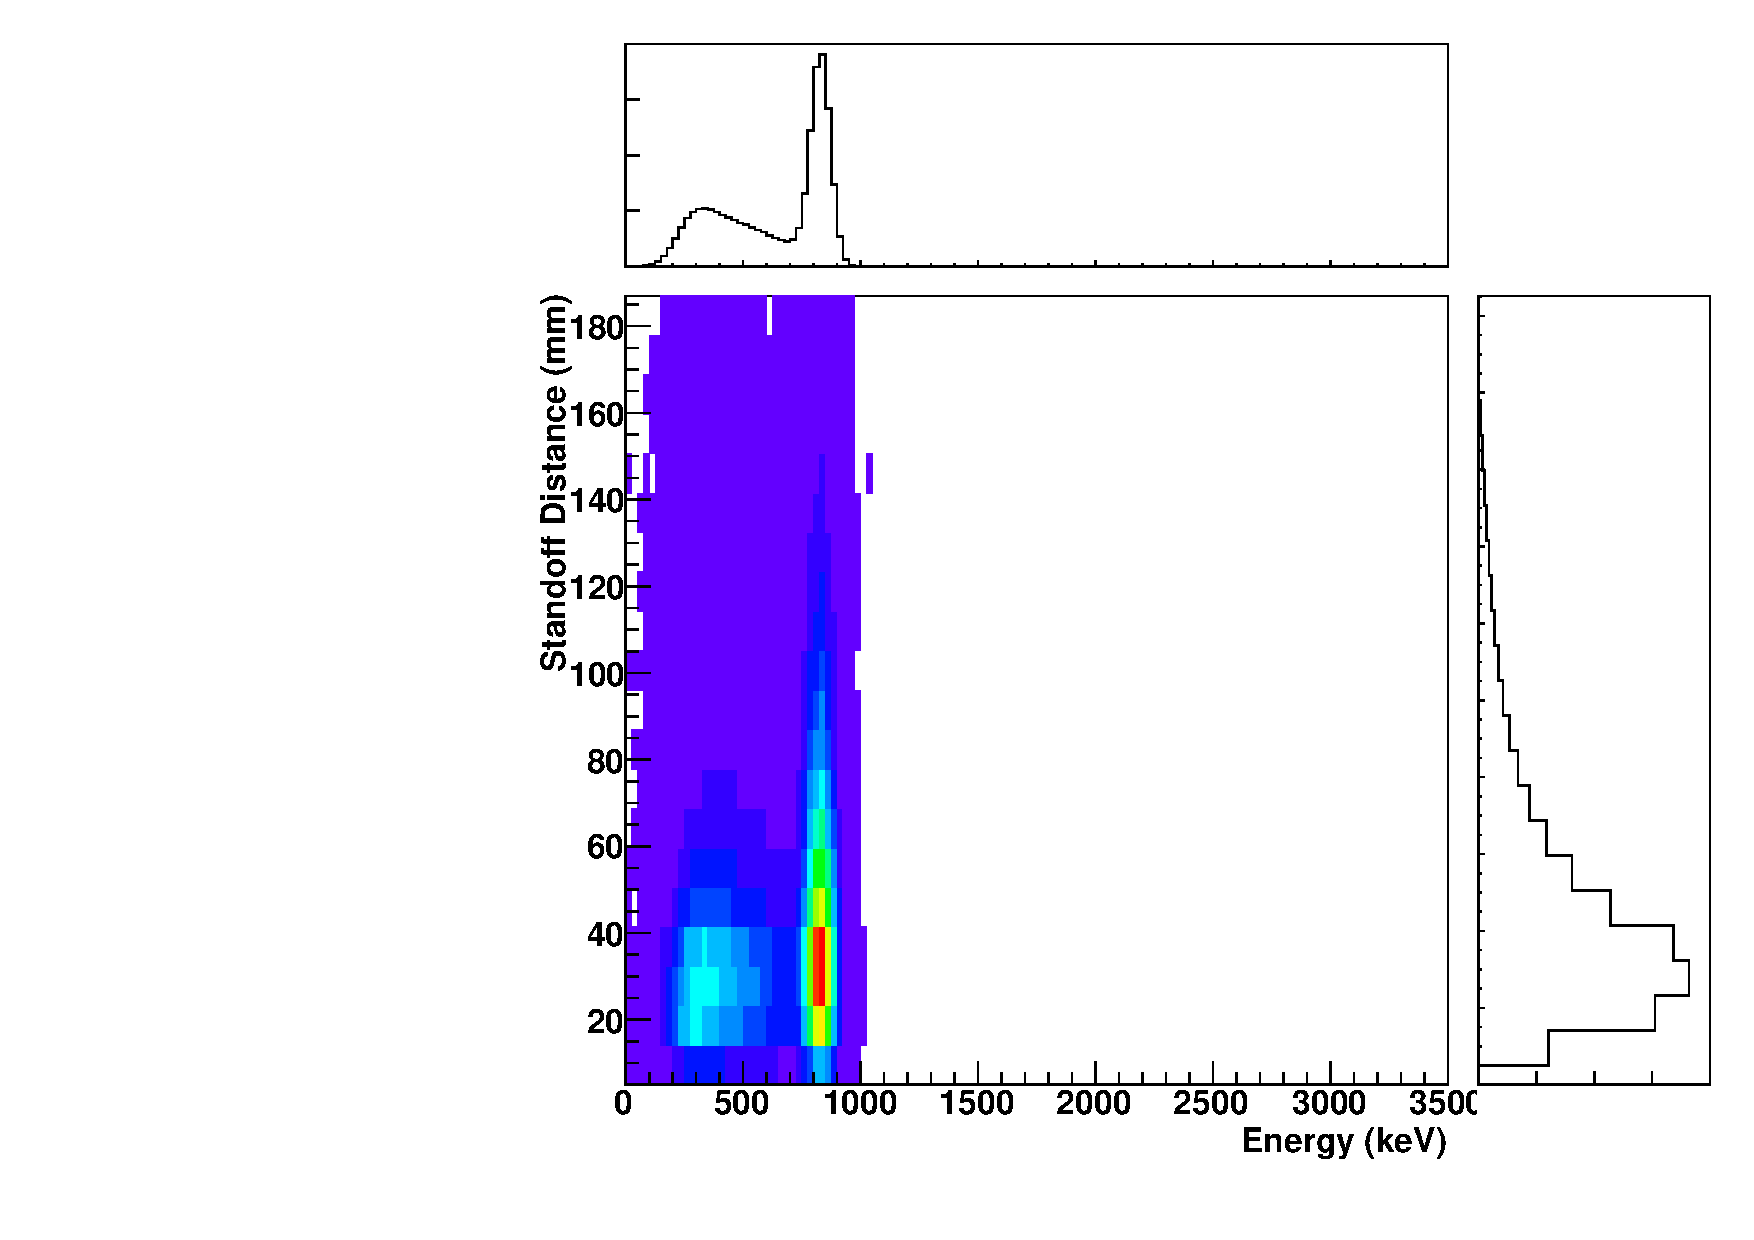
\includegraphics[width=\textwidth]{./plots/PDFs/analysis_pdf_AllVessel_Mn54_ss.pdf}
\end{subfigure}\hspace{0.1\textwidth}%
\begin{subfigure}[b]{0.35\textwidth}
	\centering
	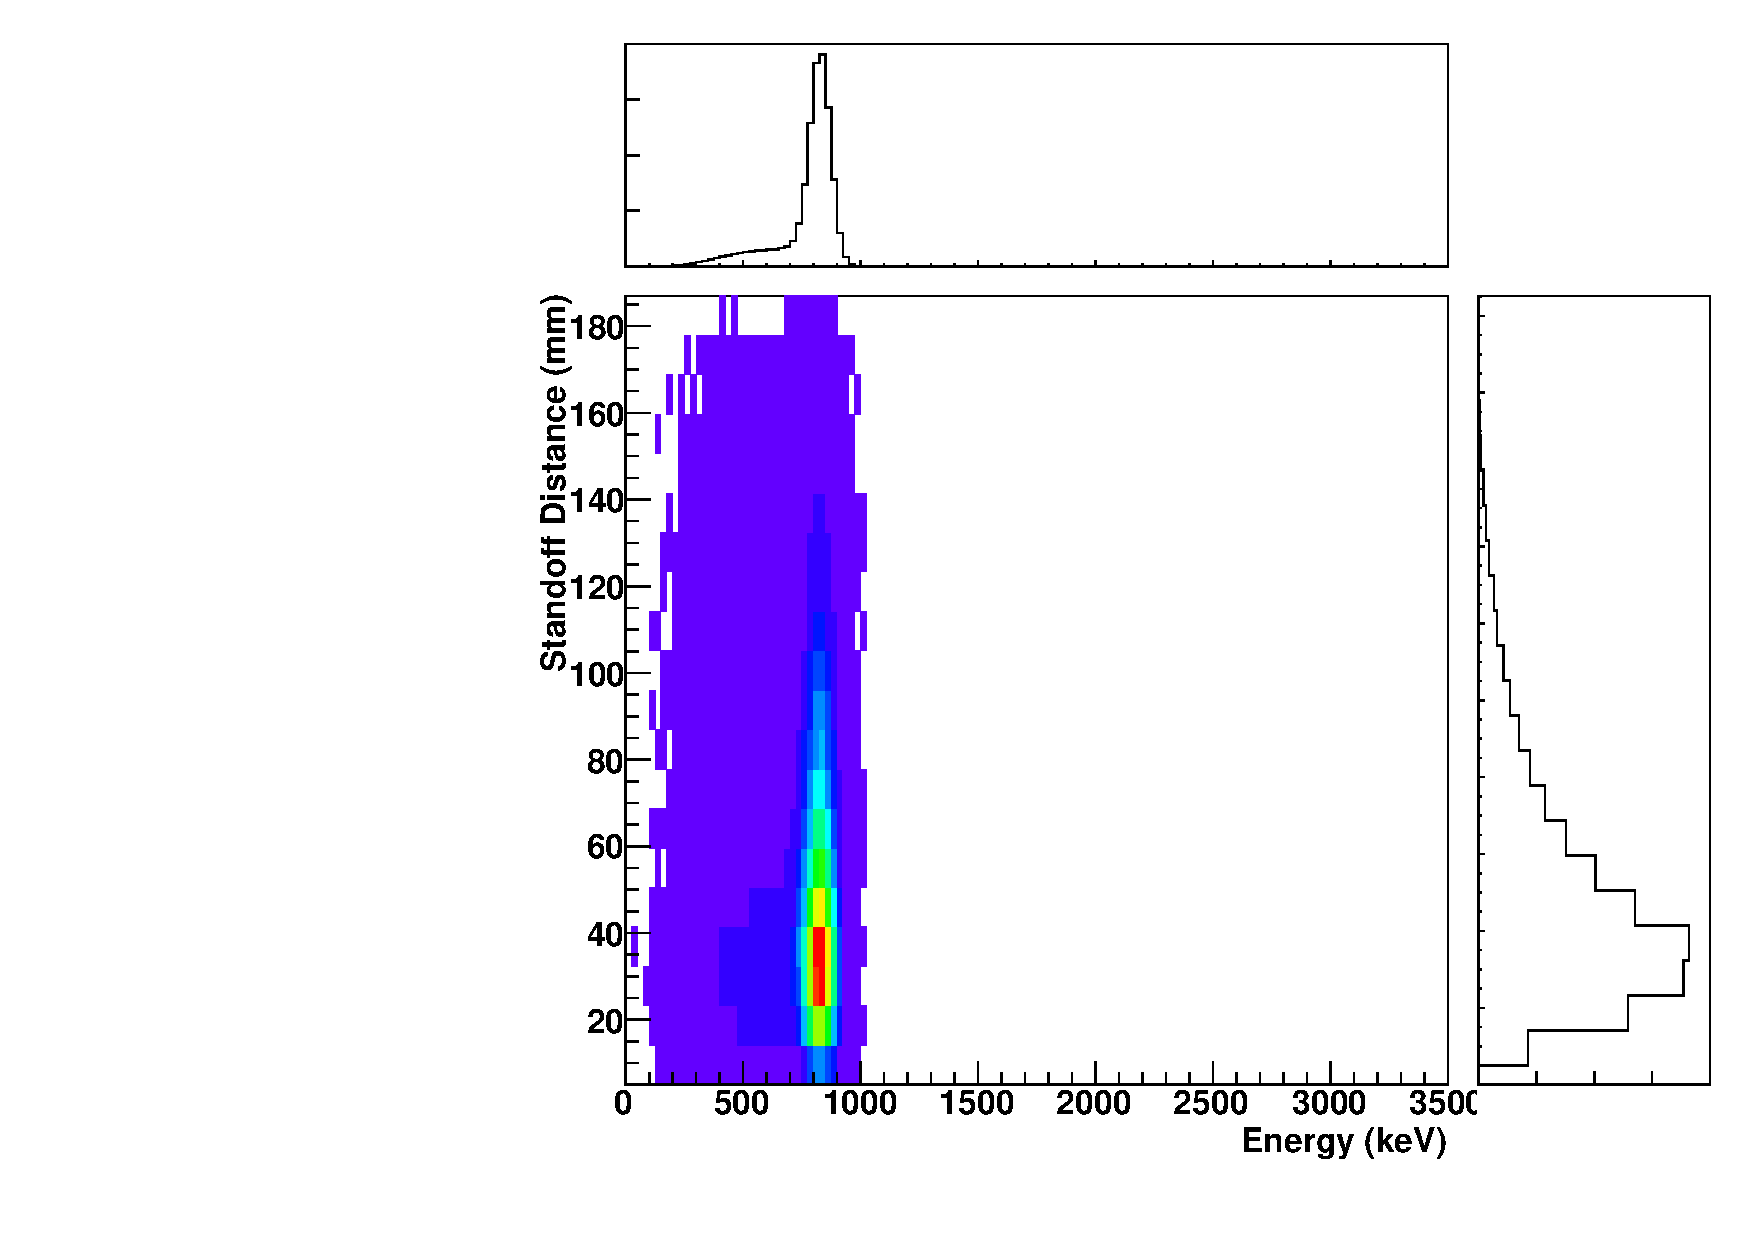
\includegraphics[width=1\textwidth]{./plots/PDFs/analysis_pdf_AllVessel_Mn54_ms.pdf}
	\end{subfigure}
\caption[PDF for \isotope{54}{Mn} in the TPC vessel]{The two dimensional PDFs for \isotope{54}{Mn} in the copper vessel, with one-dimensional projections. Single site is shown on the left, and multiple site is shown on the right.}
\label{fig:analysis_pdf_AllVessel_Mn54}
\end{figure}

\begin{figure}[hp]
\centering
	\begin{subfigure}[b]{0.35\textwidth}
	\centering
	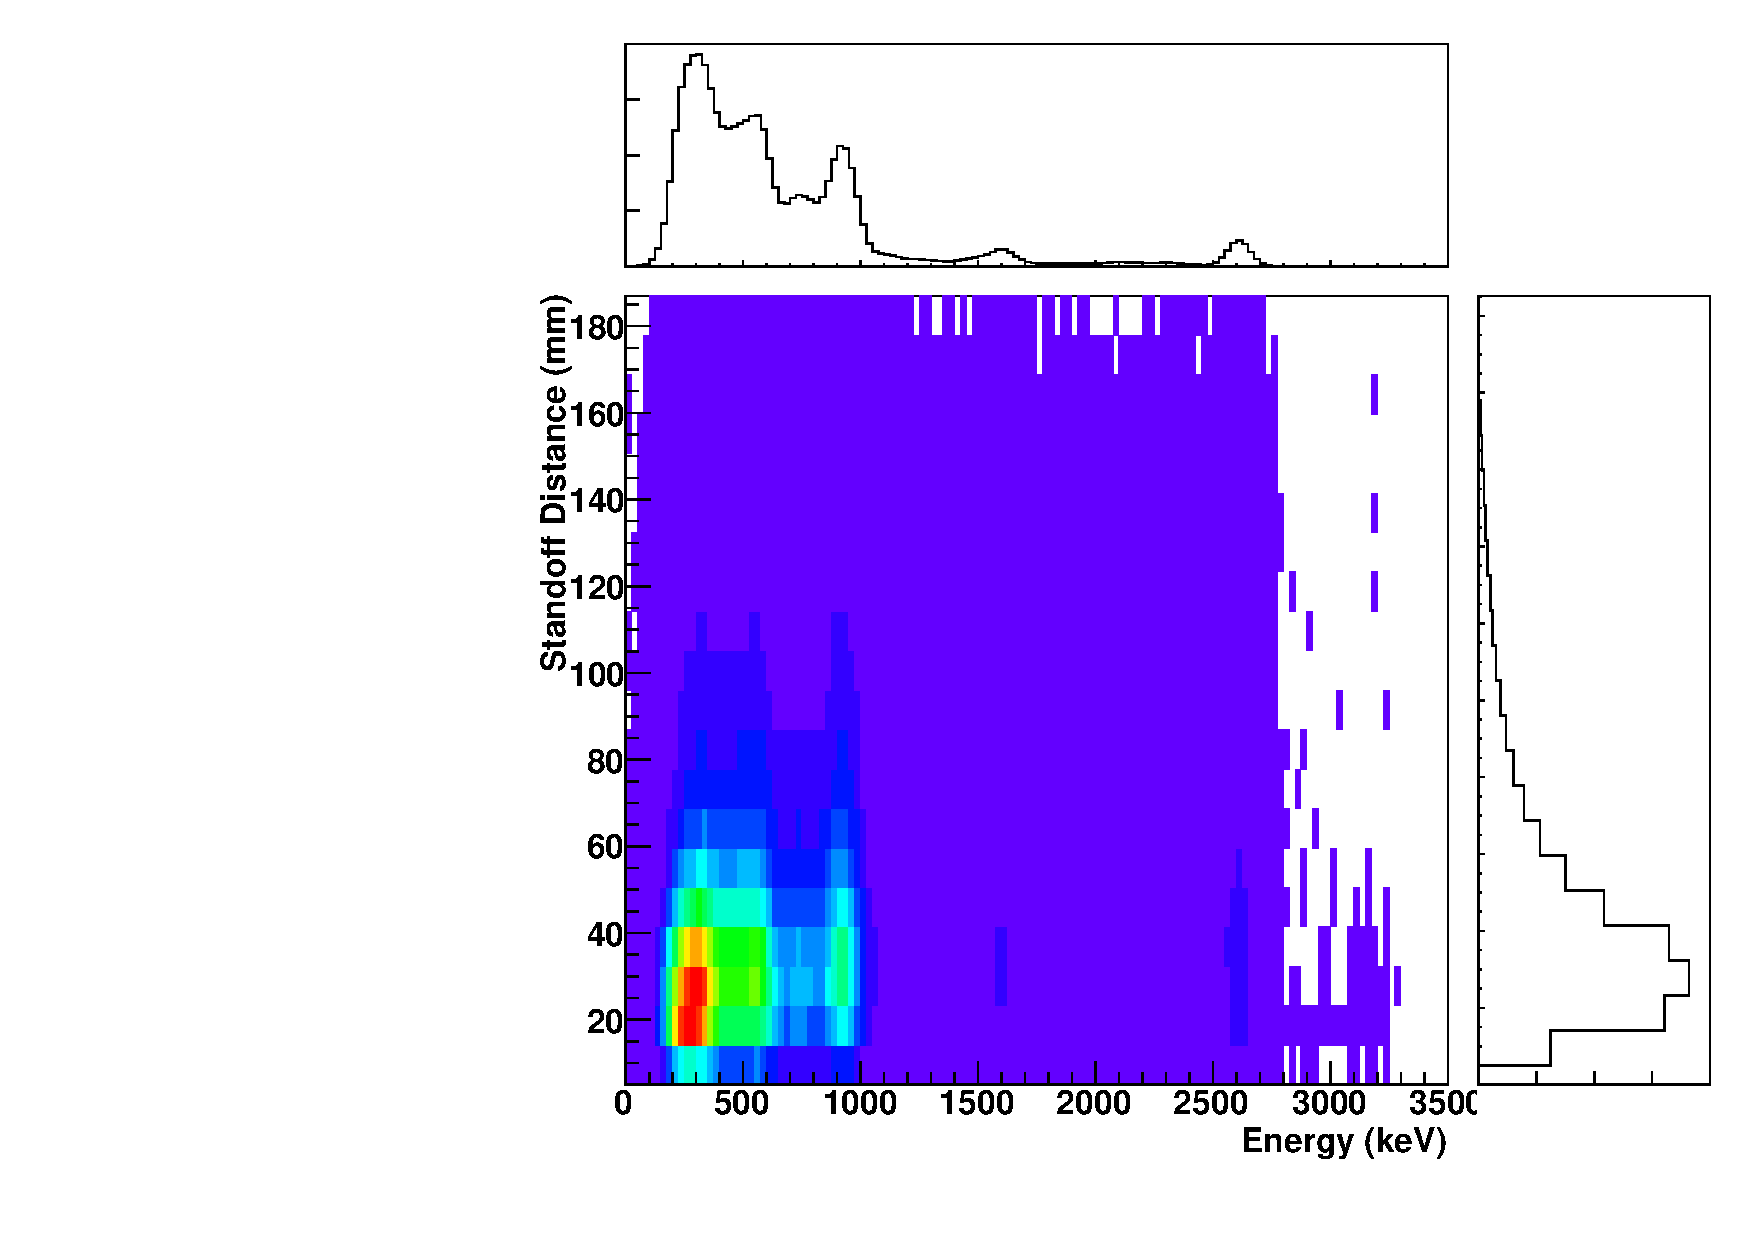
\includegraphics[width=\textwidth]{./plots/PDFs/analysis_pdf_AllVessel_Th232_ss.pdf}
\end{subfigure}\hspace{0.1\textwidth}%
\begin{subfigure}[b]{0.35\textwidth}
	\centering
	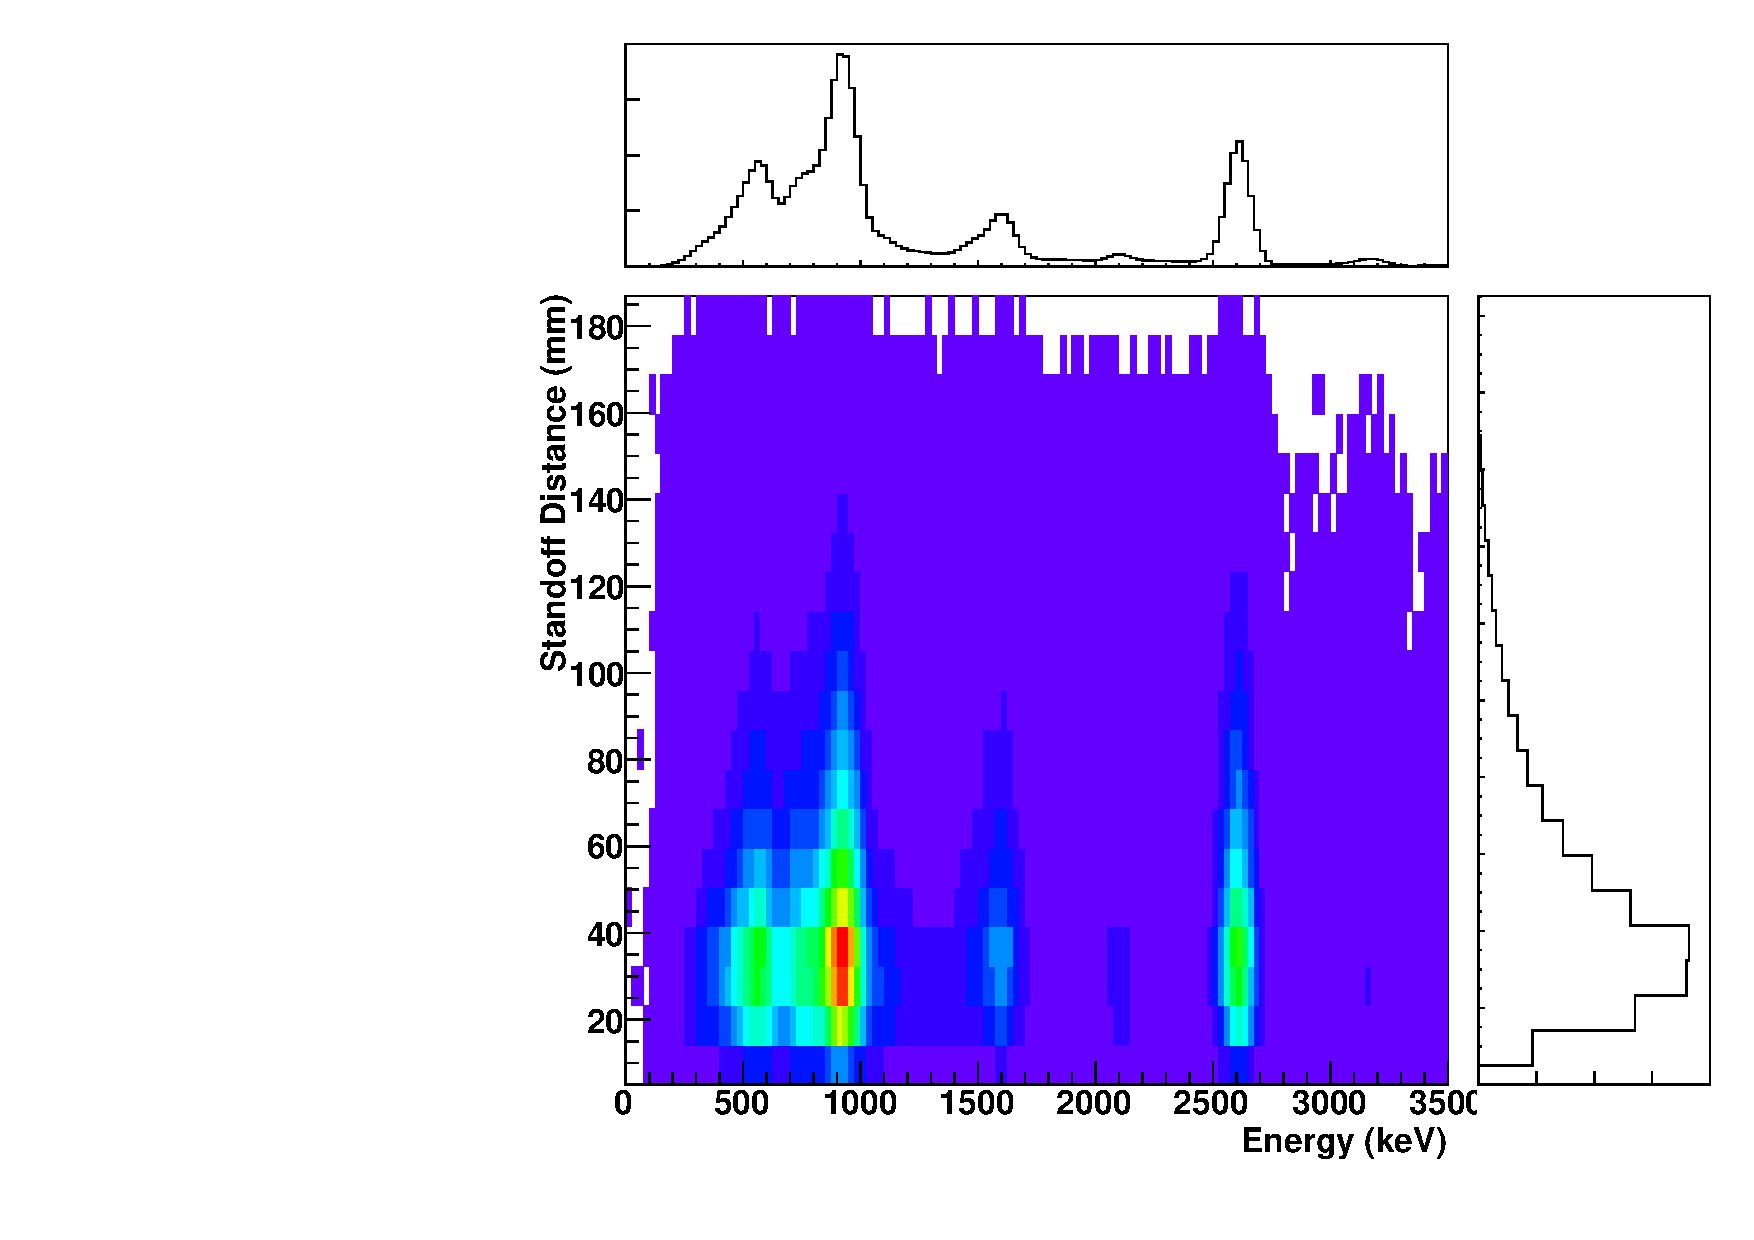
\includegraphics[width=1\textwidth]{./plots/PDFs/analysis_pdf_AllVessel_Th232_ms.pdf}
	\end{subfigure}
\caption[PDF for \isotope{232}{Th} in the TPC vessel]{The two dimensional PDFs for \isotope{232}{Th} in the copper vessel, with one-dimensional projections. Single site is shown on the left, and multiple site is shown on the right.}
\label{fig:analysis_pdf_AllVessel_Th232}
\end{figure}

\begin{figure}[hp]
\centering
	\begin{subfigure}[b]{0.35\textwidth}
	\centering
	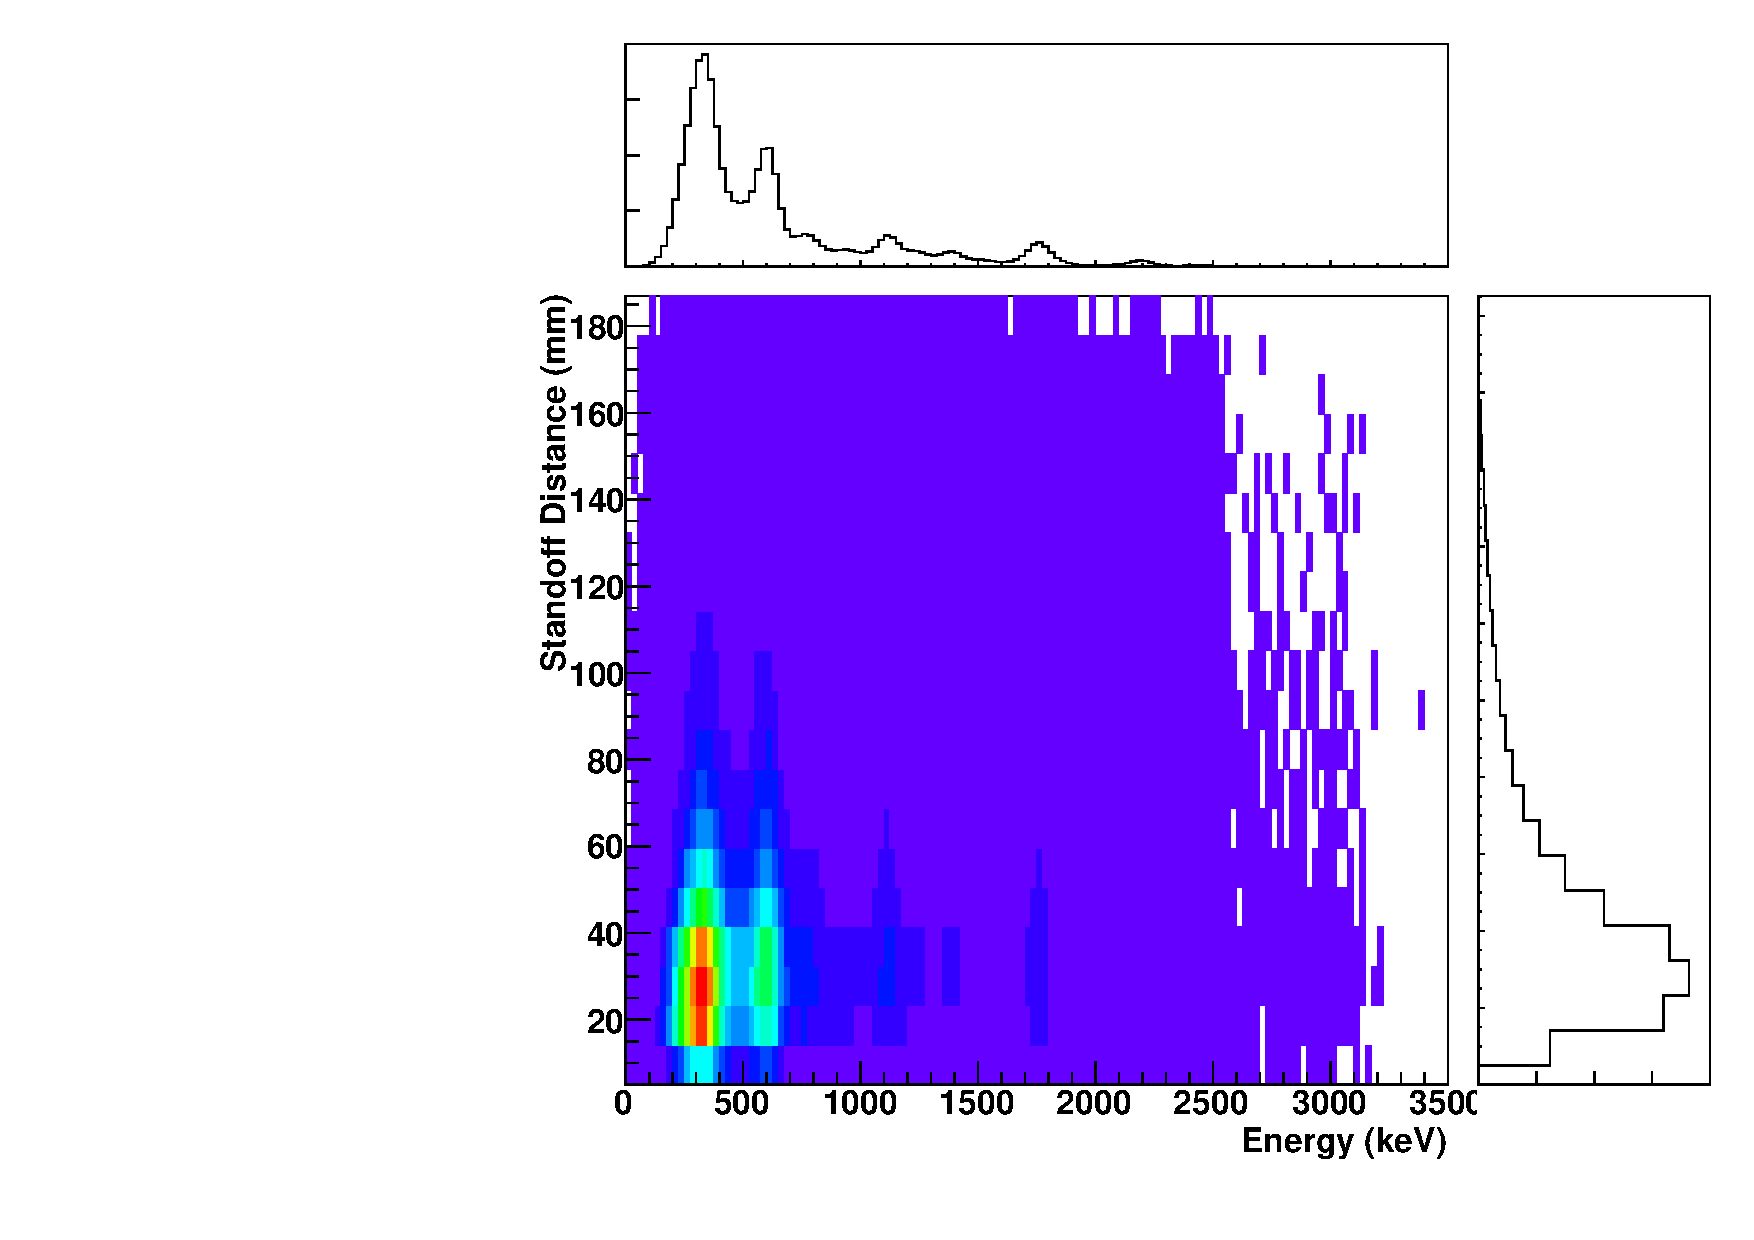
\includegraphics[width=\textwidth]{./plots/PDFs/analysis_pdf_AllVessel_U238_ss.pdf}
\end{subfigure}\hspace{0.1\textwidth}%
\begin{subfigure}[b]{0.35\textwidth}
	\centering
	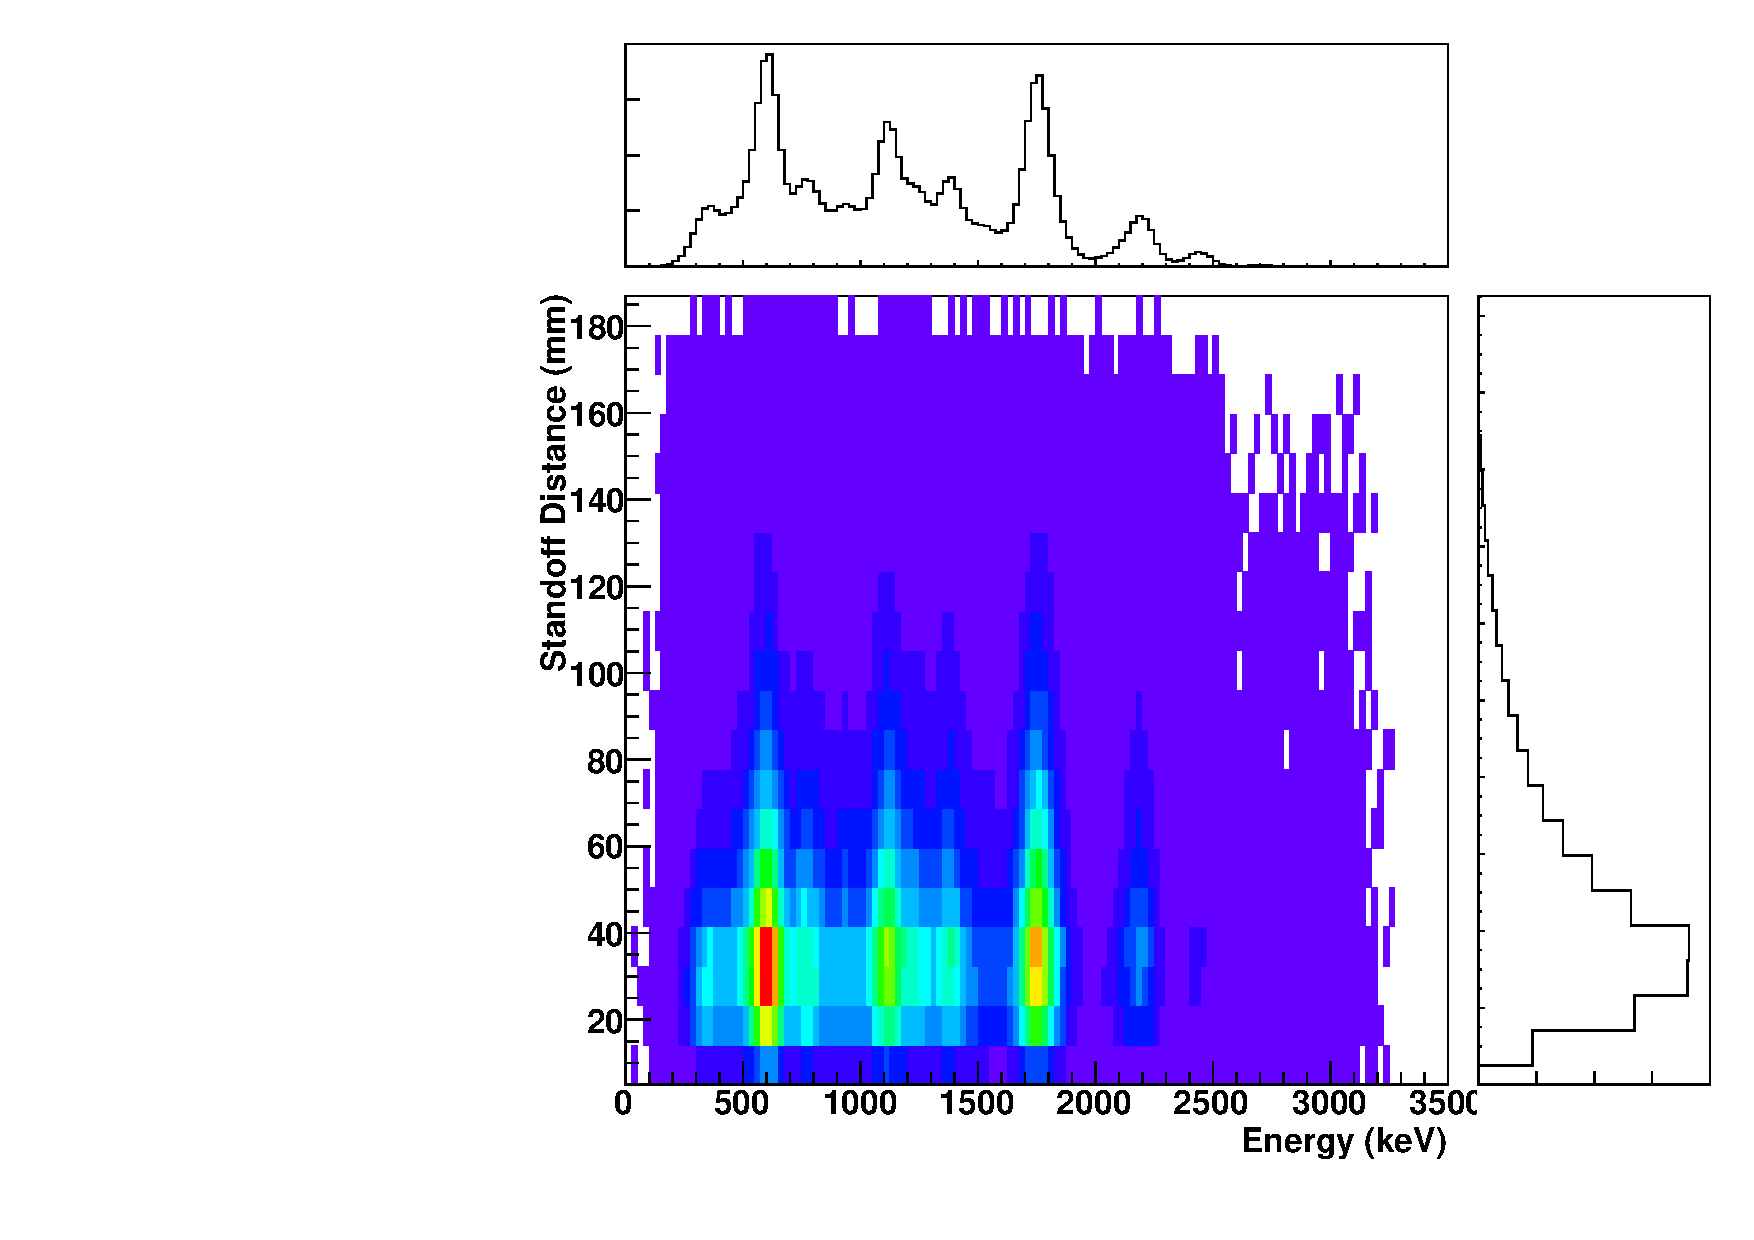
\includegraphics[width=1\textwidth]{./plots/PDFs/analysis_pdf_AllVessel_U238_ms.pdf}
	\end{subfigure}
\caption[PDF for \isotope{238}{U} in the TPC vessel]{The two dimensional PDFs for \isotope{238}{U} in the copper vessel, with one-dimensional projections. Single site is shown on the left, and multiple site is shown on the right.}
\label{fig:analysis_pdf_AllVessel_U238}
\end{figure}

\begin{figure}[hp]
\centering
	\begin{subfigure}[b]{0.35\textwidth}
	\centering
	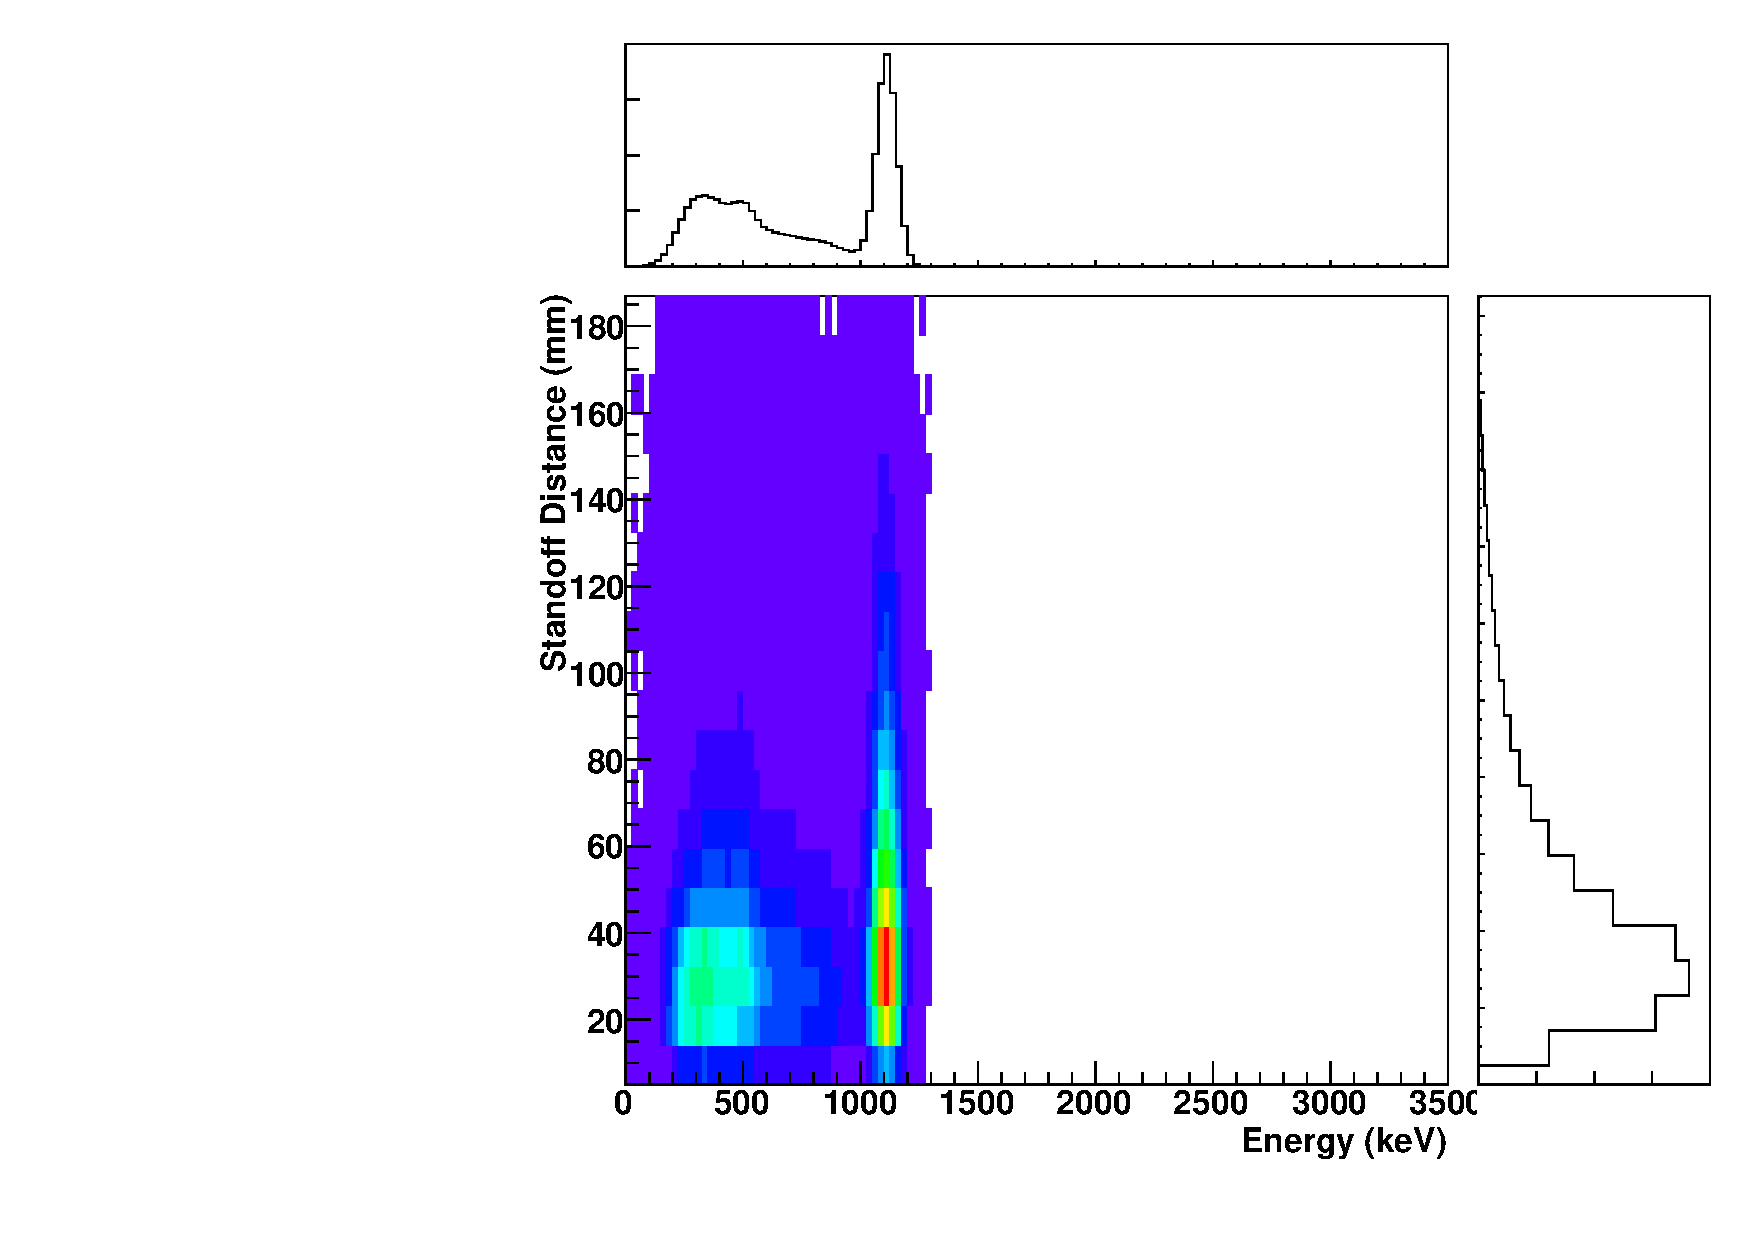
\includegraphics[width=\textwidth]{./plots/PDFs/analysis_pdf_AllVessel_Zn65_ss.pdf}
\end{subfigure}\hspace{0.1\textwidth}%
\begin{subfigure}[b]{0.35\textwidth}
	\centering
	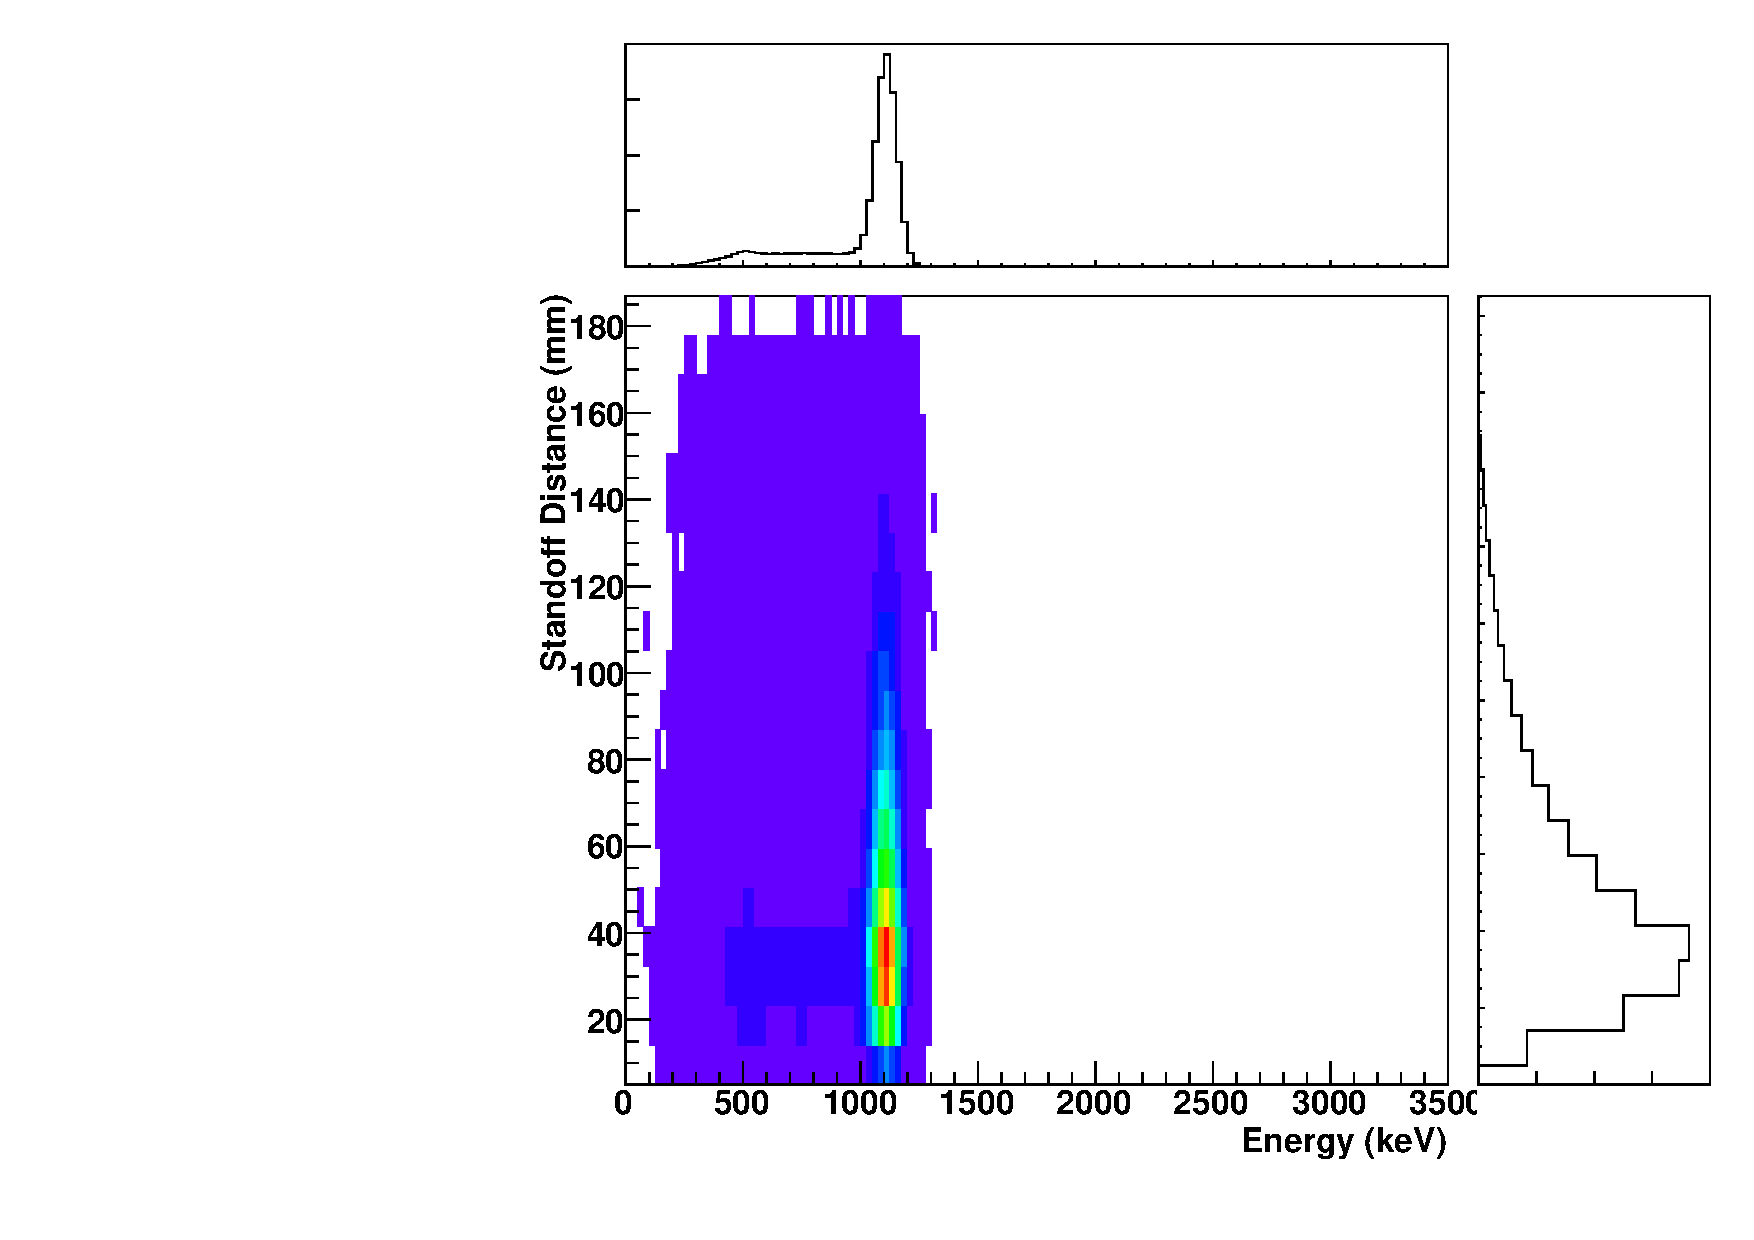
\includegraphics[width=1\textwidth]{./plots/PDFs/analysis_pdf_AllVessel_Zn65_ms.pdf}
	\end{subfigure}
\caption[PDF for \isotope{65}{Zn} in the TPC vessel]{The two dimensional PDFs for \isotope{65}{Zn} in the copper vessel, with one-dimensional projections. Single site is shown on the left, and multiple site is shown on the right.}
\label{fig:analysis_pdf_AllVessel_Zn65}
\end{figure}

\begin{figure}[hp]
\centering
	\begin{subfigure}[b]{0.35\textwidth}
	\centering
	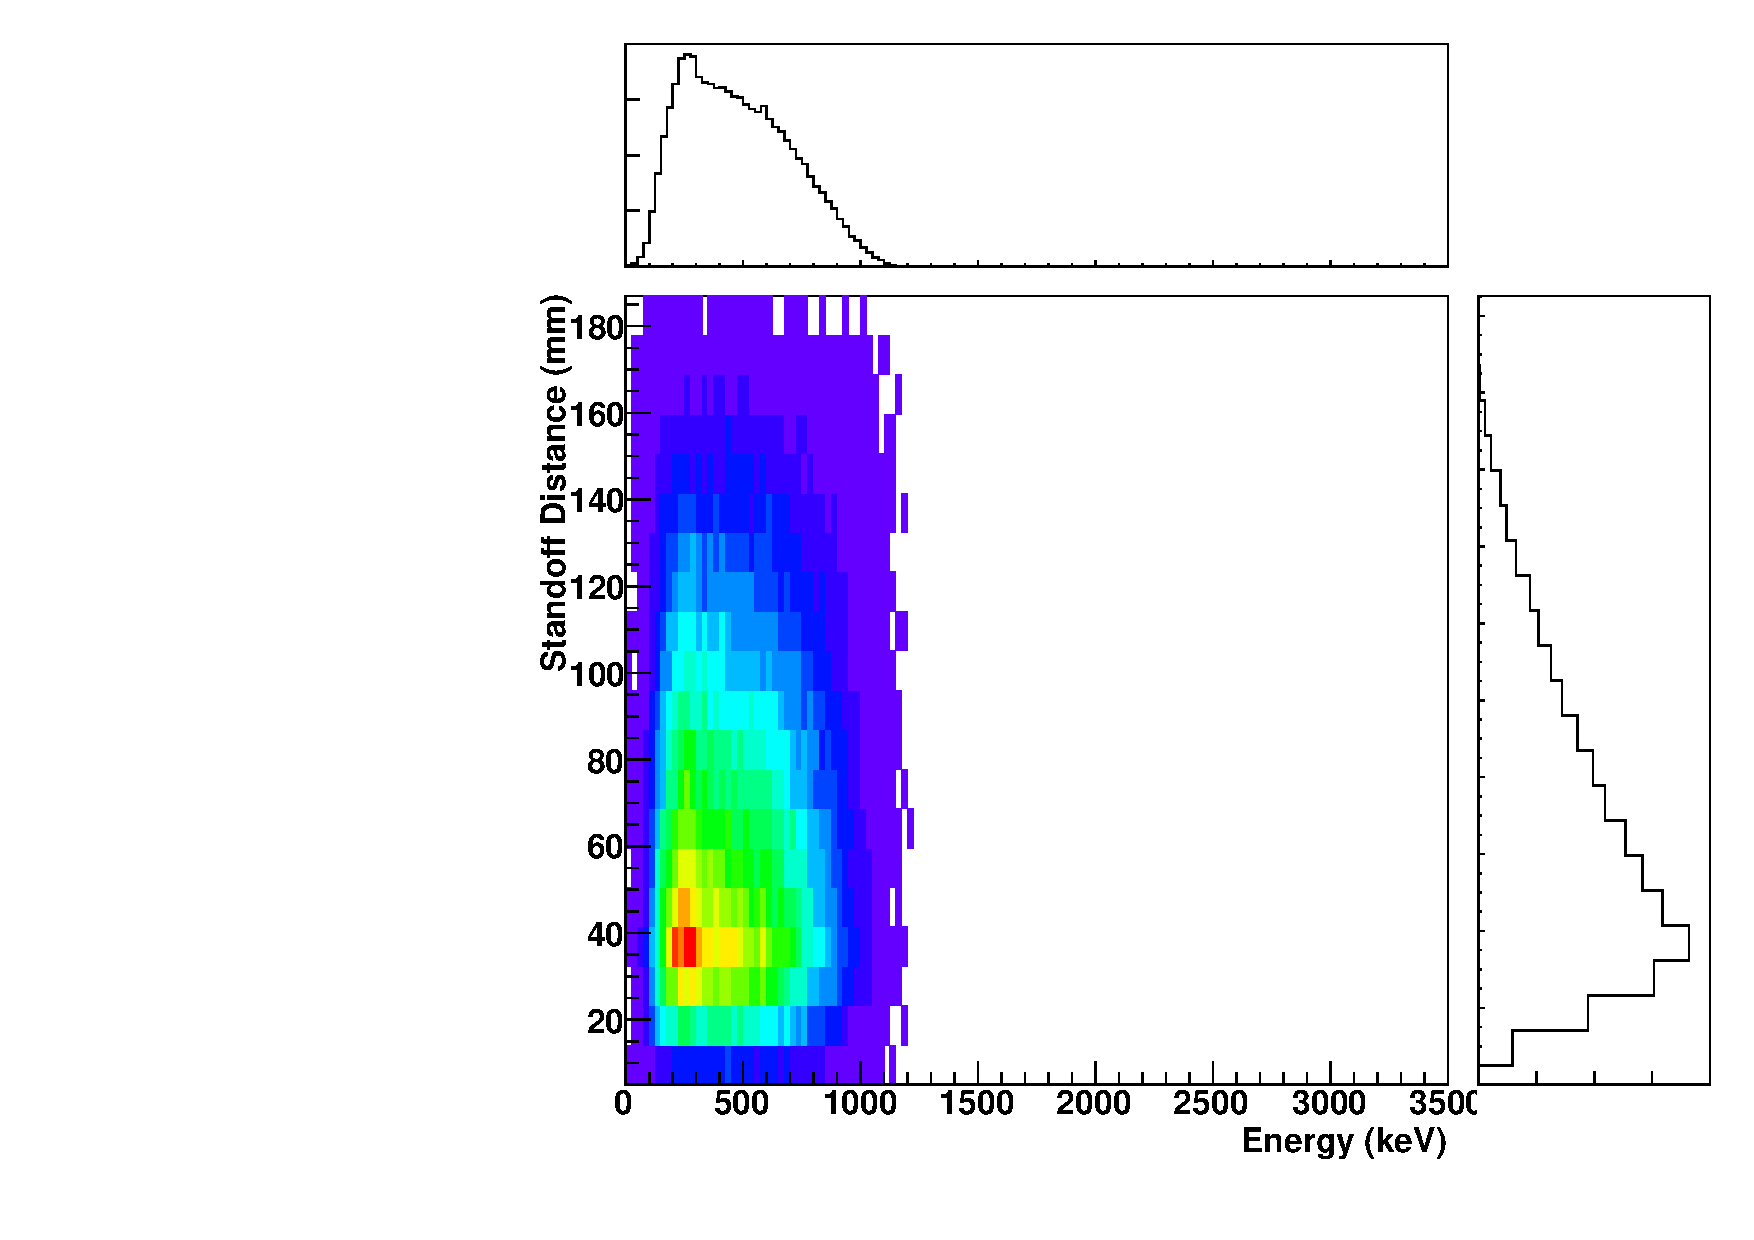
\includegraphics[width=\textwidth]{./plots/PDFs/analysis_pdf_ActiveLXe_Xe135_ss.pdf}
\end{subfigure}\hspace{0.1\textwidth}%
\begin{subfigure}[b]{0.35\textwidth}
	\centering
	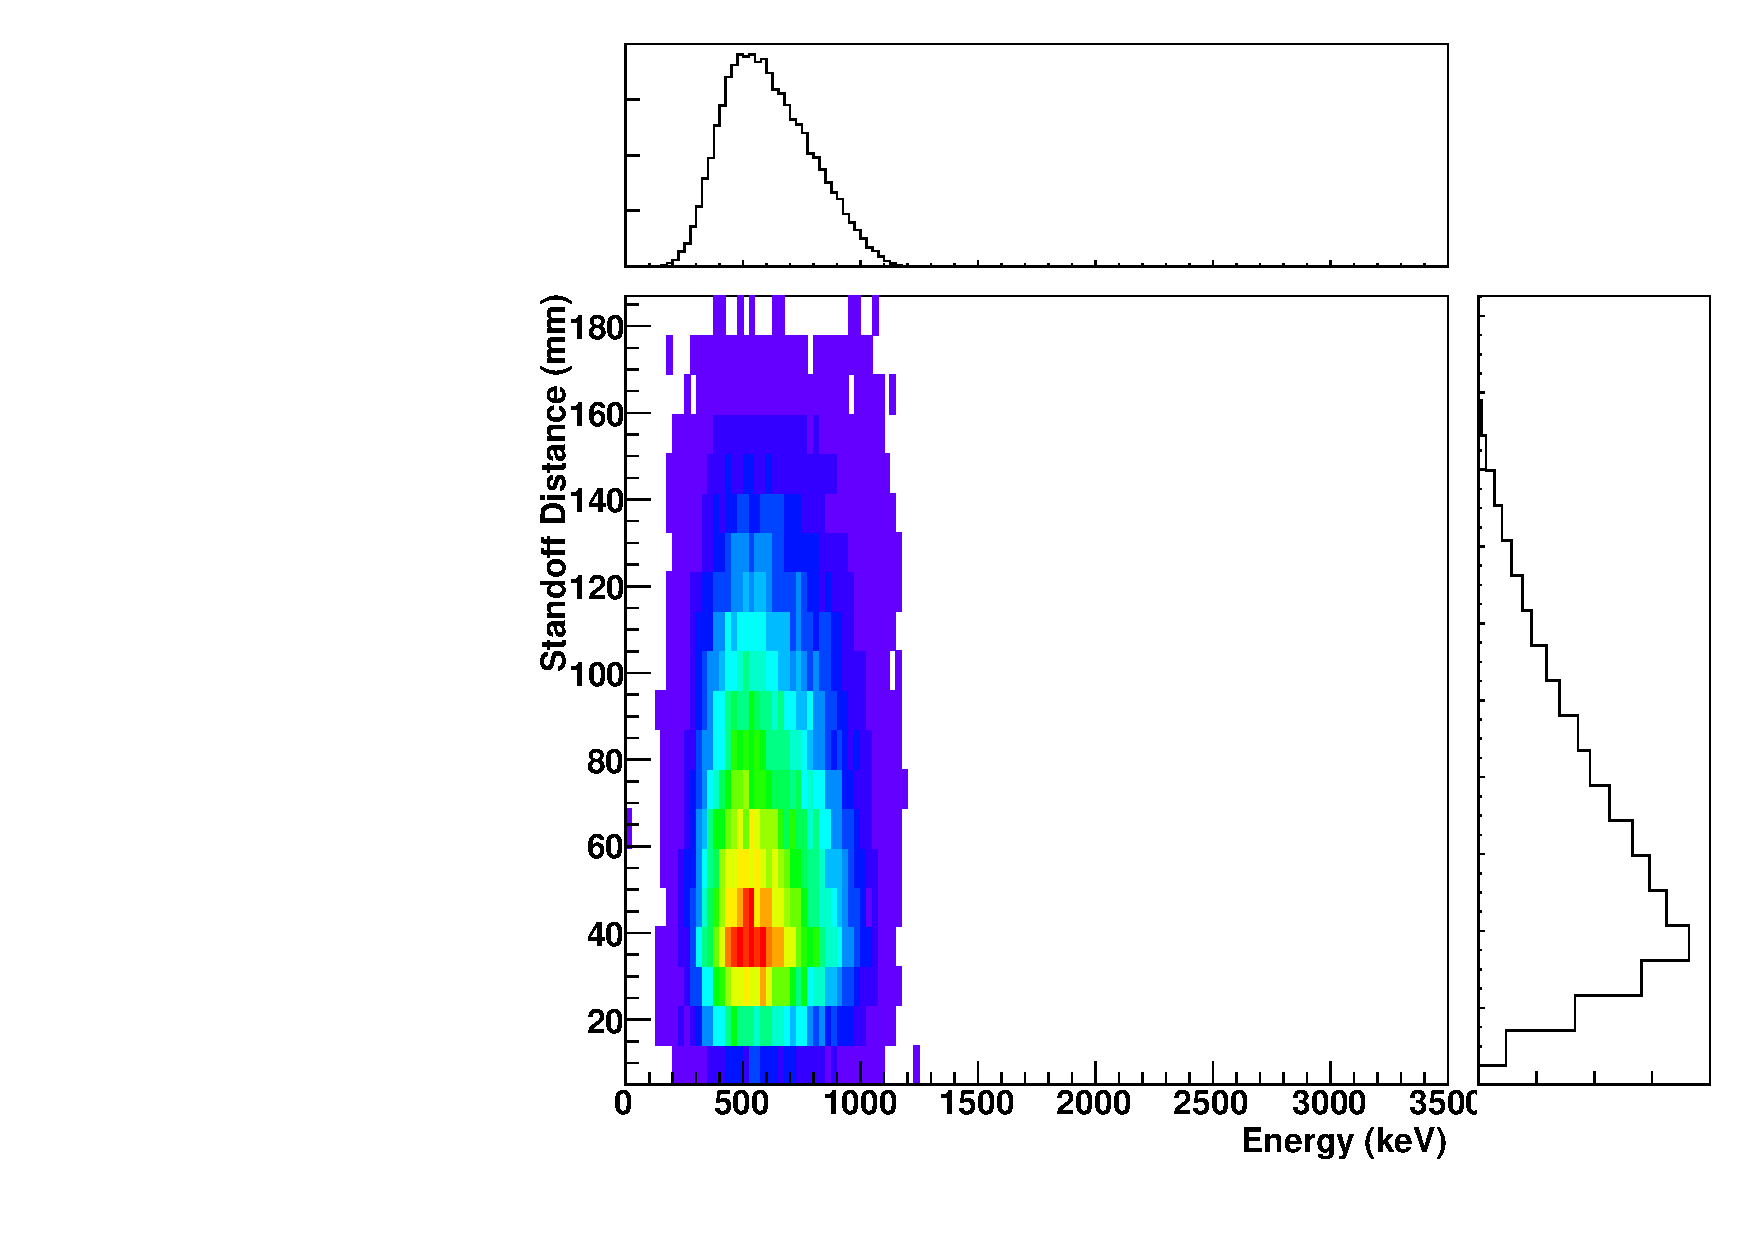
\includegraphics[width=1\textwidth]{./plots/PDFs/analysis_pdf_ActiveLXe_Xe135_ms.pdf}
	\end{subfigure}
\caption[PDF for \isotope{135}{Xe} in the active xenon]{The two dimensional PDFs for \isotope{135}{Xe} in the active xenon, with one-dimensional projections. Single site is shown on the left, and multiple site is shown on the right.}
\label{fig:analysis_pdf_ActiveLXe_Xe135}
\end{figure}

\begin{figure}[hp]
\centering
	\begin{subfigure}[b]{0.35\textwidth}
	\centering
	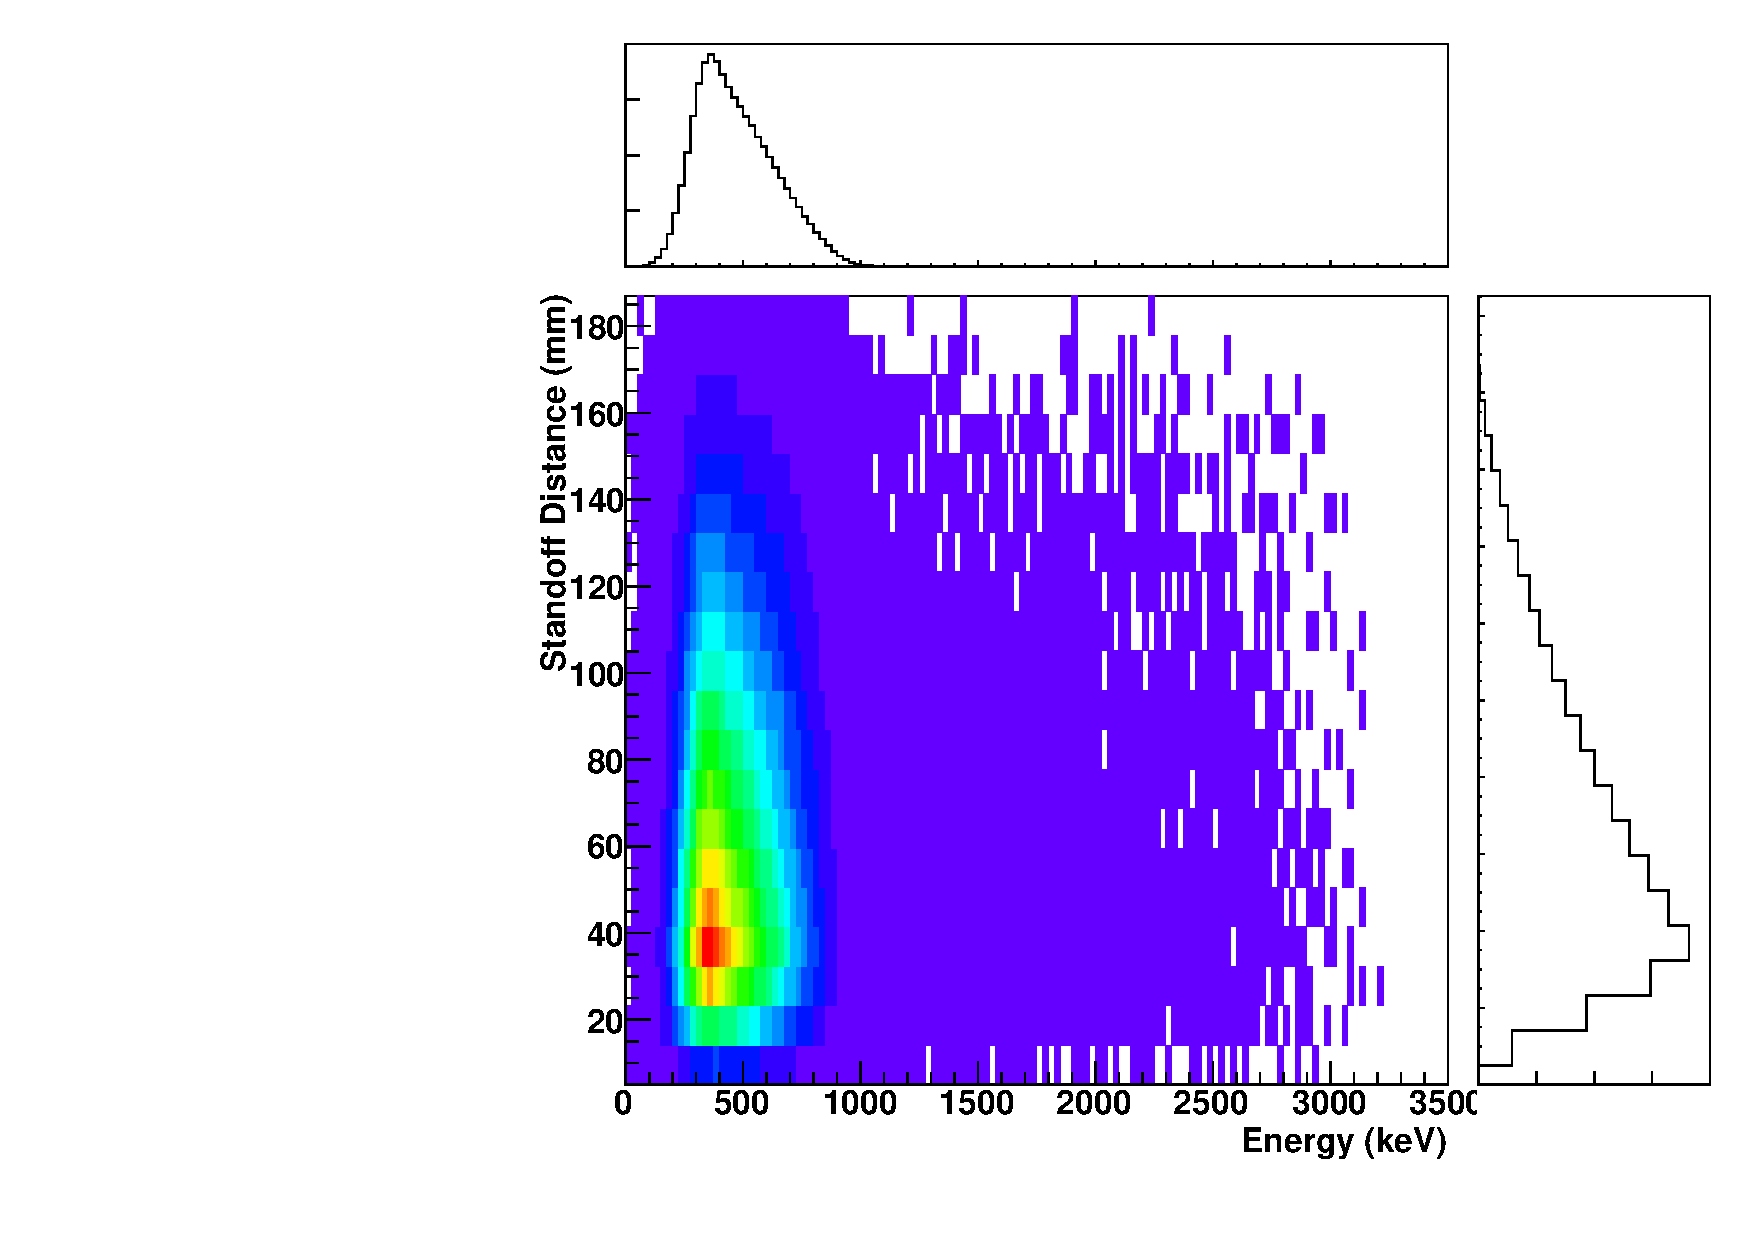
\includegraphics[width=\textwidth]{./plots/PDFs/analysis_pdf_ActiveLXe_Rn222_ss.pdf}
\end{subfigure}\hspace{0.1\textwidth}%
\begin{subfigure}[b]{0.35\textwidth}
	\centering
	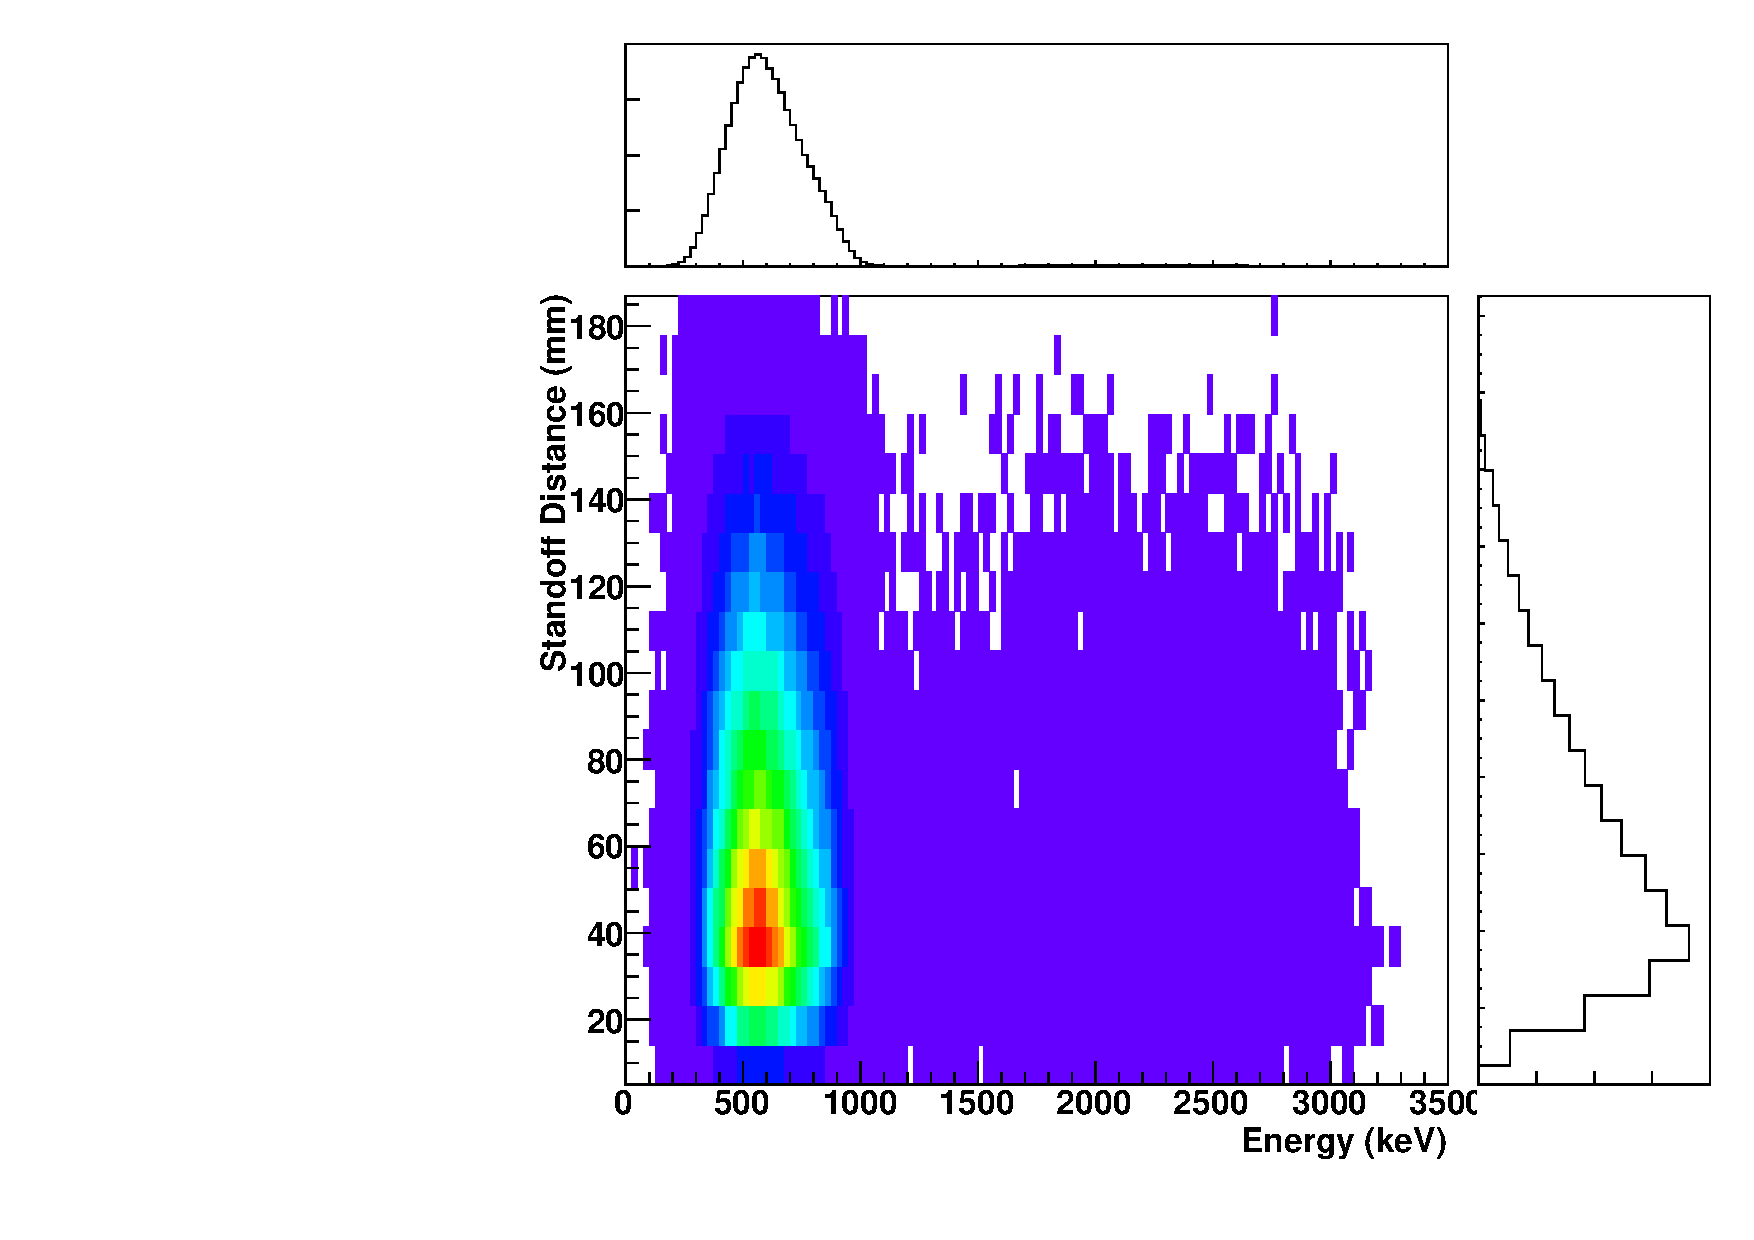
\includegraphics[width=1\textwidth]{./plots/PDFs/analysis_pdf_ActiveLXe_Rn222_ms.pdf}
	\end{subfigure}
\caption[PDF for \isotope{222}{Rn} in the active xenon]{The two dimensional PDFs for \isotope{222}{Rn} in the active xenon, with one-dimensional projections. Single site is shown on the left, and multiple site is shown on the right.}
\label{fig:analysis_pdf_ActiveLXe_Rn222}
\end{figure}

\begin{figure}[hp]
\centering
	\begin{subfigure}[b]{0.35\textwidth}
	\centering
	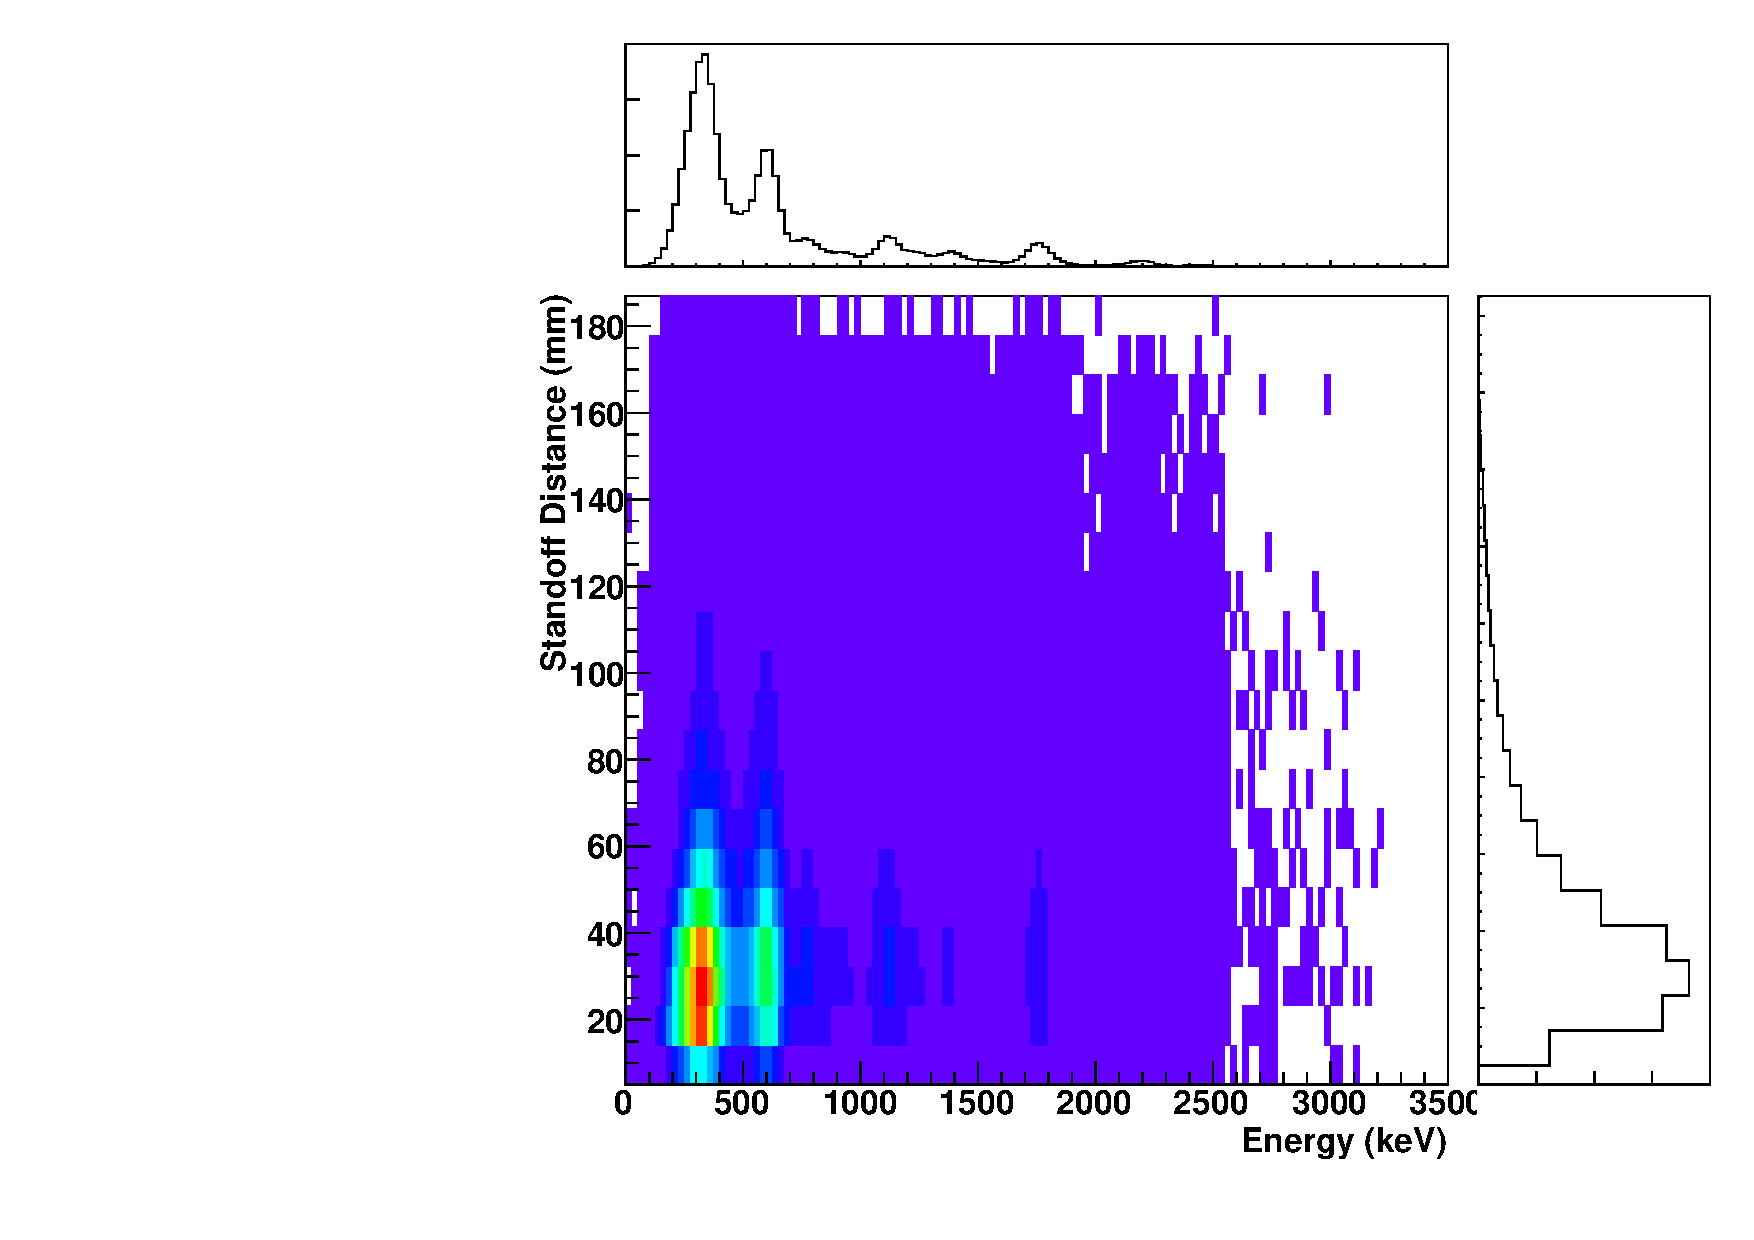
\includegraphics[width=\textwidth]{./plots/PDFs/analysis_pdf_InactiveLXe_Rn222_ss.pdf}
\end{subfigure}\hspace{0.1\textwidth}%
\begin{subfigure}[b]{0.35\textwidth}
	\centering
	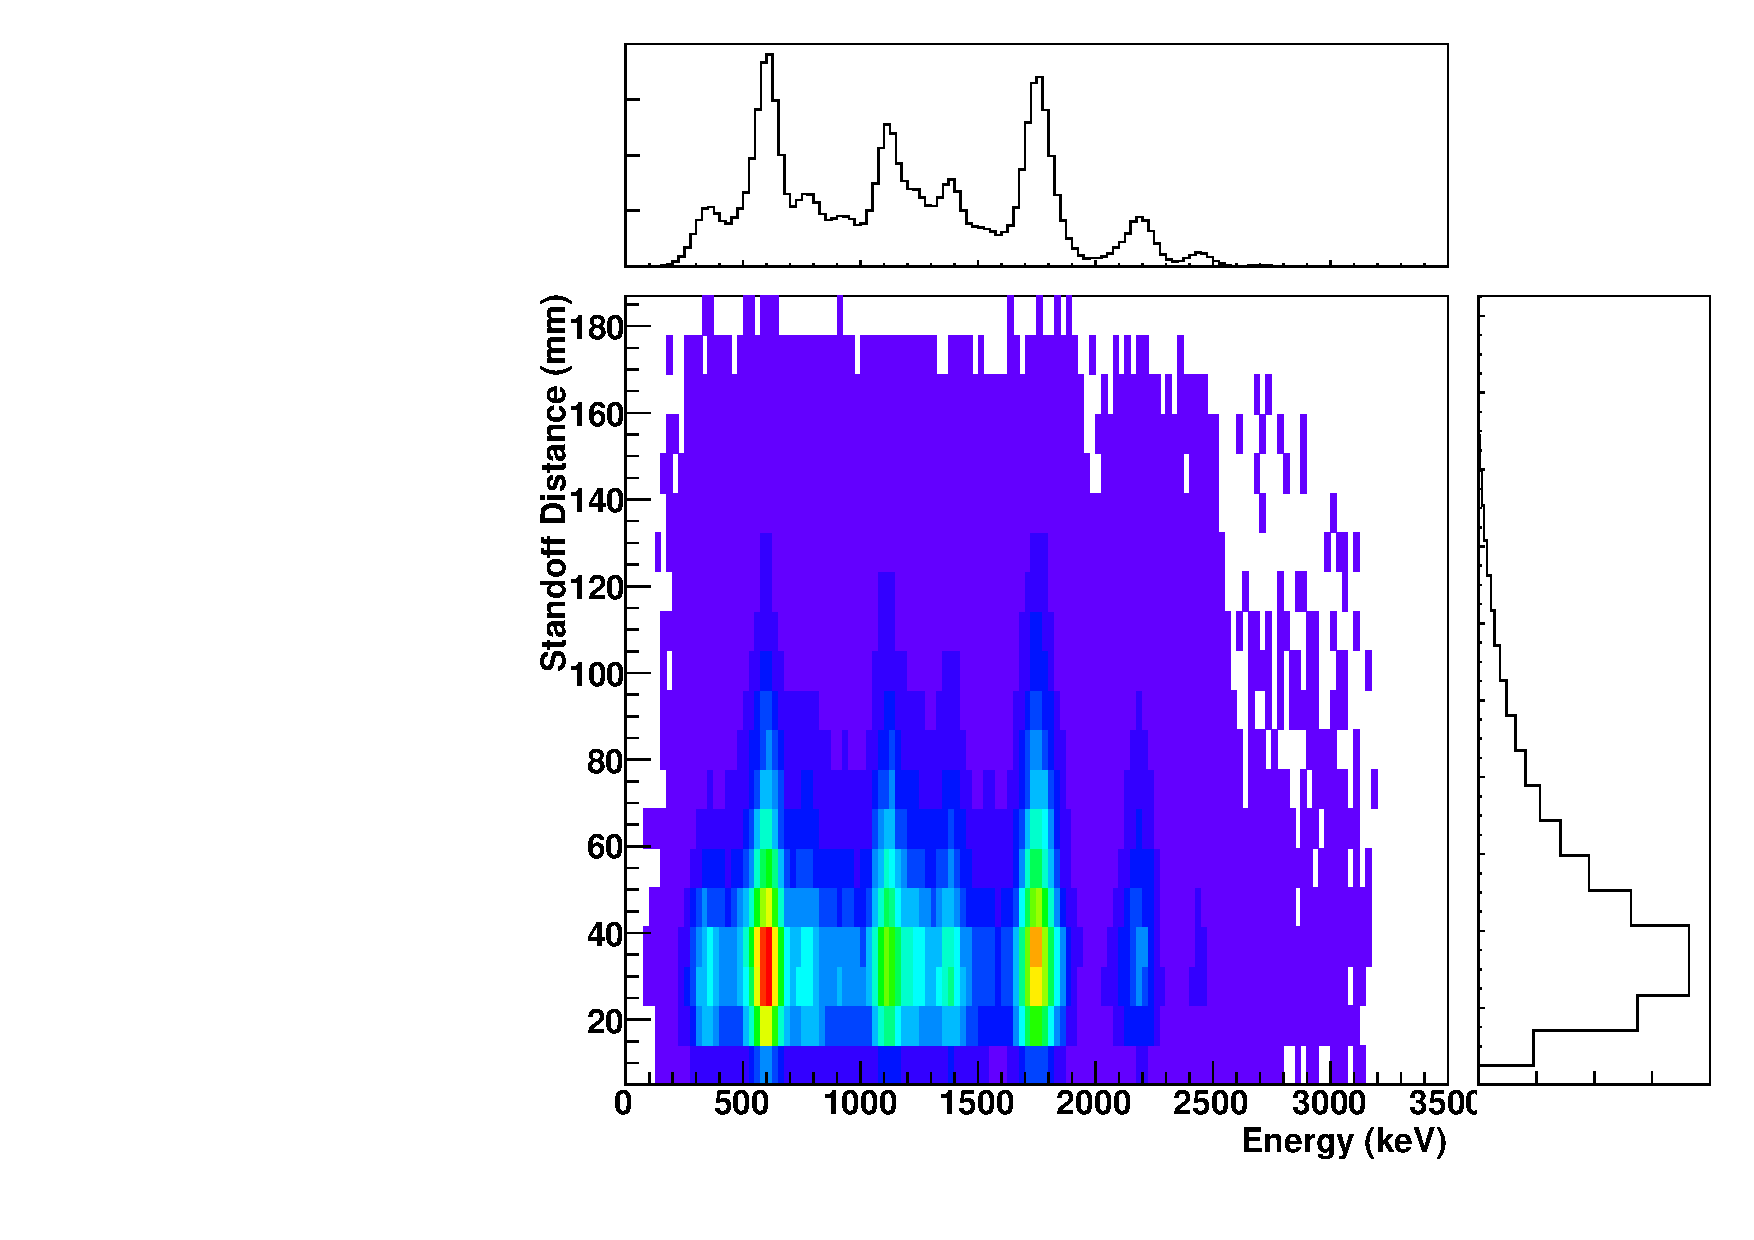
\includegraphics[width=1\textwidth]{./plots/PDFs/analysis_pdf_InactiveLXe_Rn222_ms.pdf}
	\end{subfigure}
\caption[PDF for \isotope{222}{Rn} in the inactive xenon]{The two dimensional PDFs for \isotope{222}{Rn} in the inactive xenon, with one-dimensional projections. Single site is shown on the left, and multiple site is shown on the right.}
\label{fig:analysis_pdf_InactiveLXe_Rn222}
\end{figure}

\begin{figure}[hp]
\centering
	\begin{subfigure}[b]{0.35\textwidth}
	\centering
	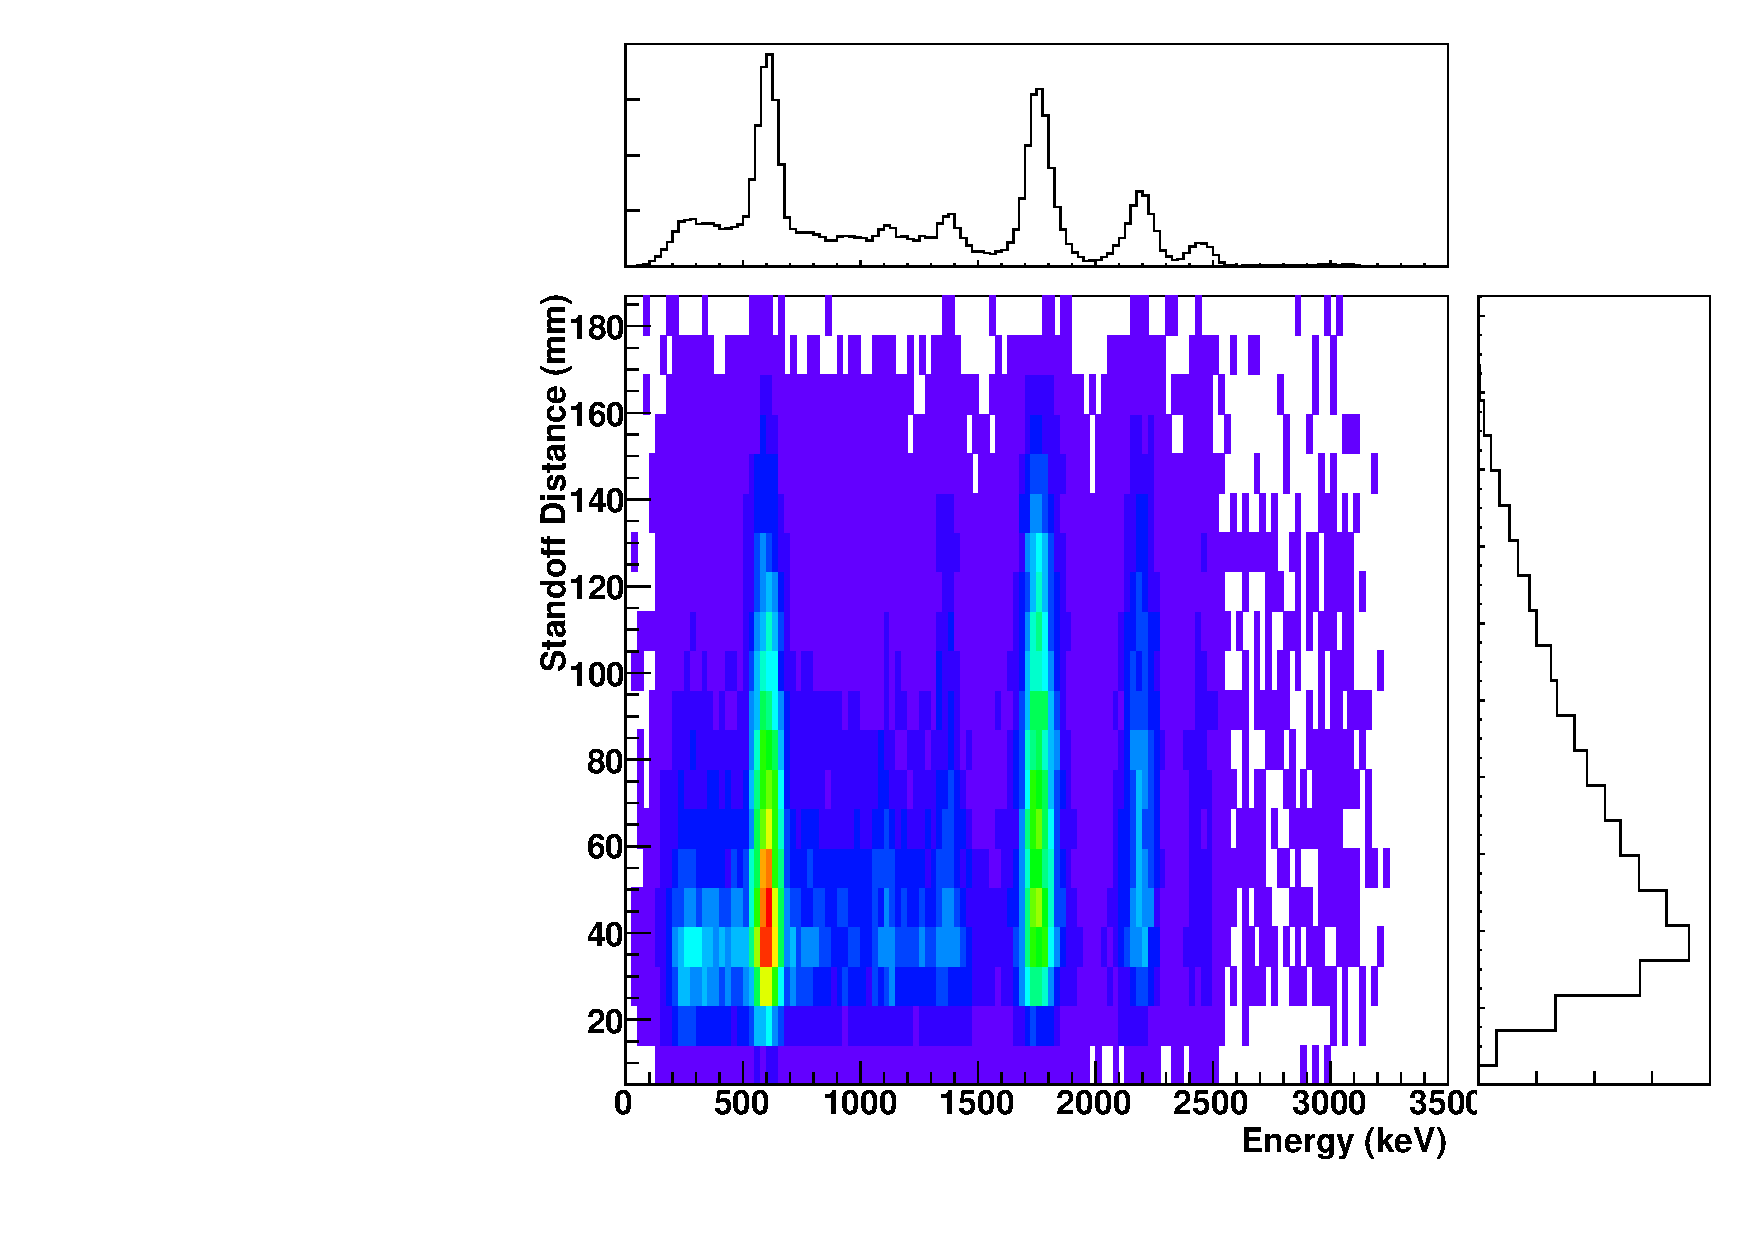
\includegraphics[width=\textwidth]{./plots/PDFs/analysis_pdf_CathodeSurf_Bi214_nochain_ss.pdf}
\end{subfigure}\hspace{0.1\textwidth}%
\begin{subfigure}[b]{0.35\textwidth}
	\centering
	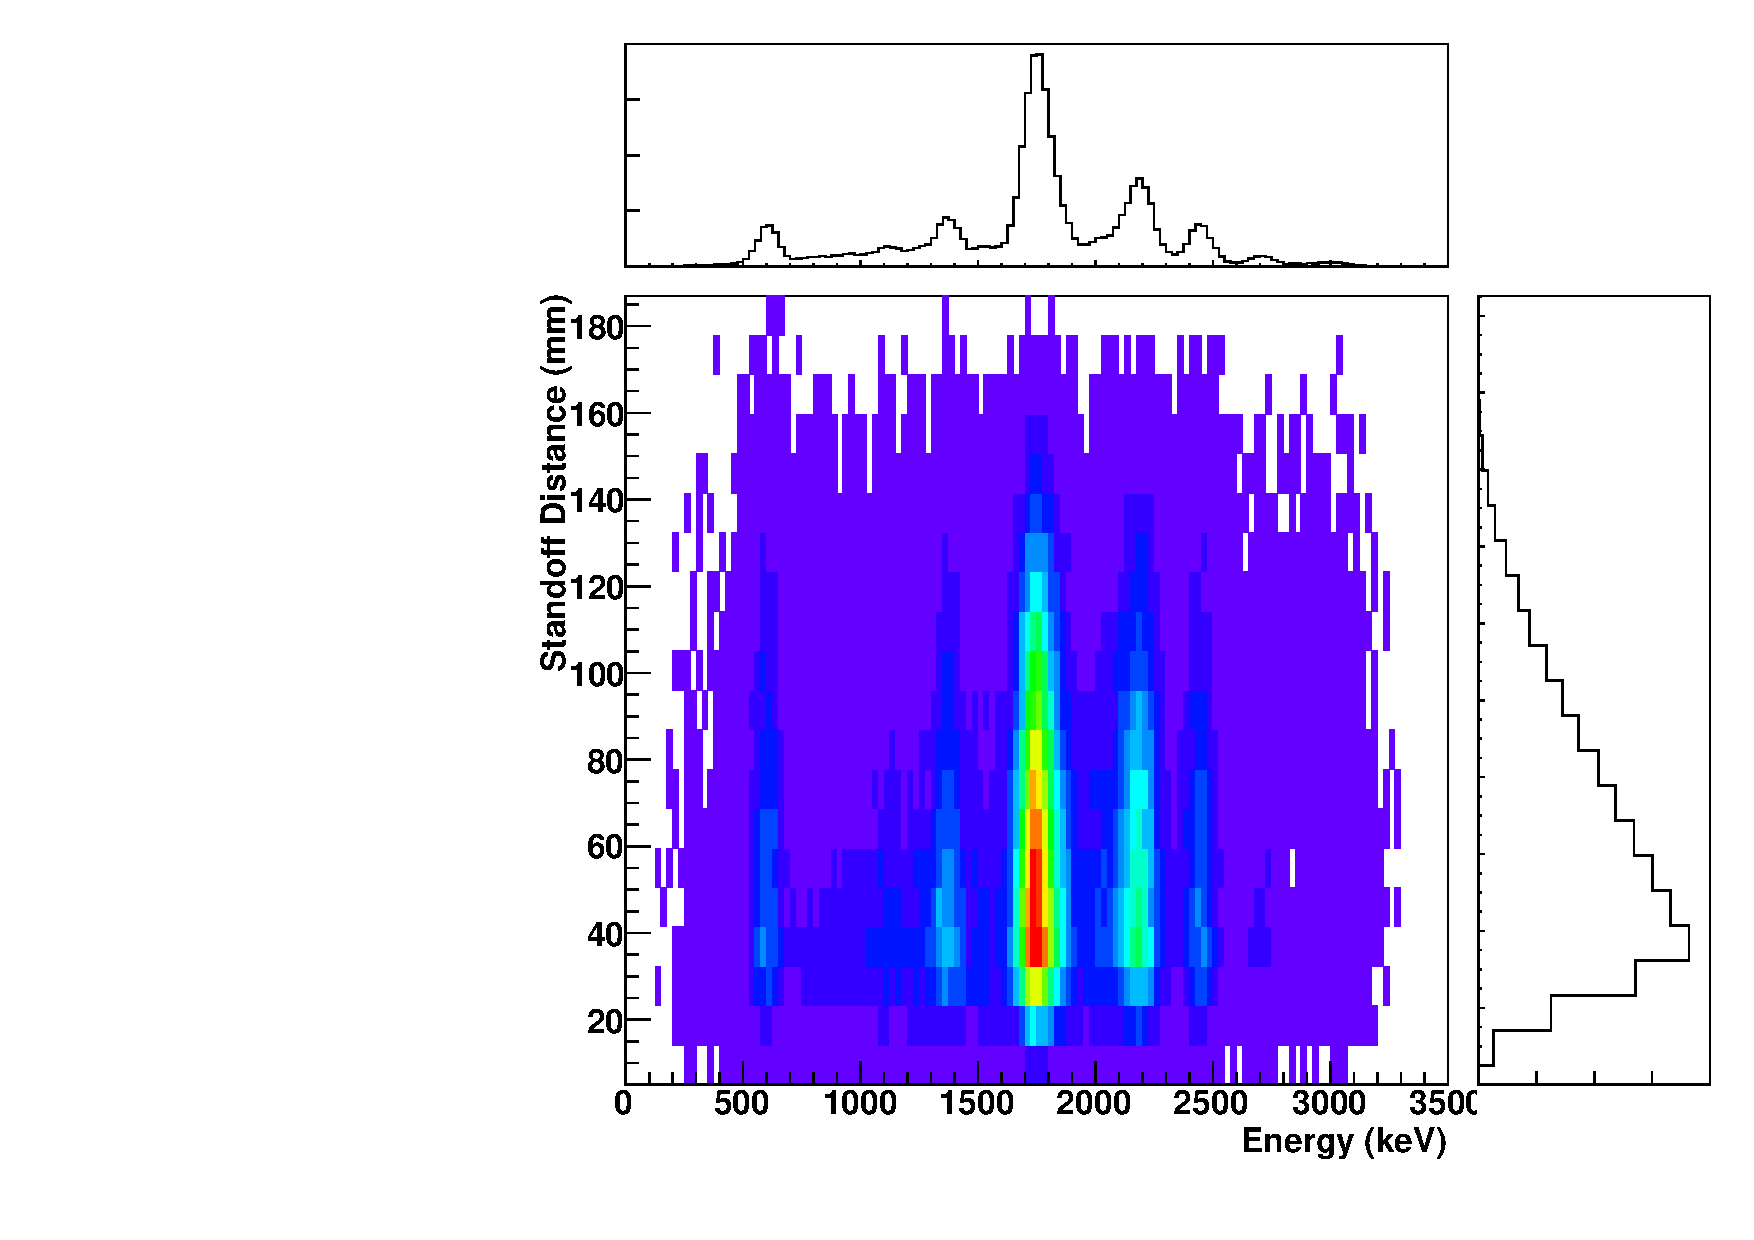
\includegraphics[width=1\textwidth]{./plots/PDFs/analysis_pdf_CathodeSurf_Bi214_nochain_ms.pdf}
	\end{subfigure}
\caption[PDF for \isotope{214}{Bi} on the cathode]{The two dimensional PDFs for \isotope{214}{Bi} on the cathode due to drifting daughters of \isotope{222}{Rn}, with one-dimensional projections. Single site is shown on the left, and multiple site is shown on the right.}
\label{fig:analysis_pdf_CathodeSurf_Bi214_nochain}
\end{figure}

\begin{figure}[hp]
\centering
	\begin{subfigure}[b]{0.35\textwidth}
	\centering
	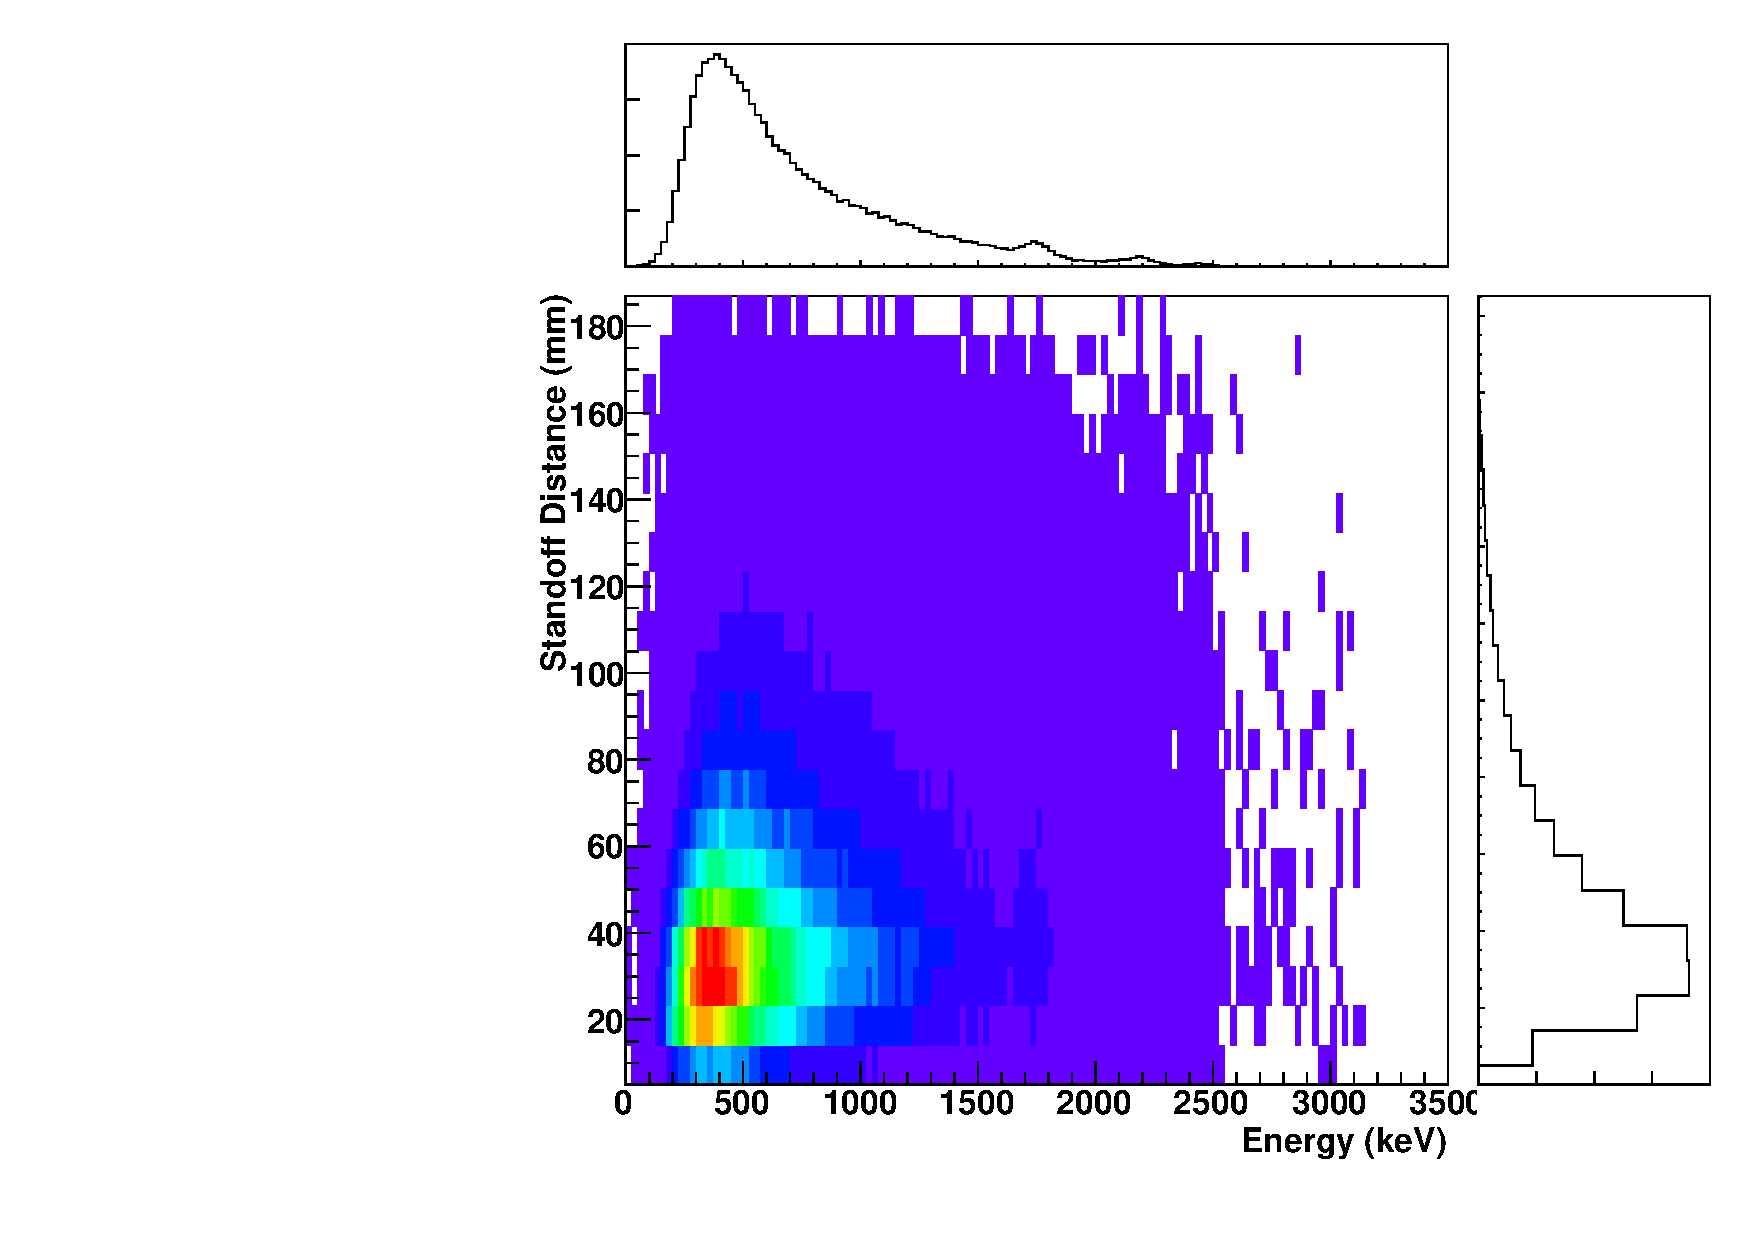
\includegraphics[width=\textwidth]{./plots/PDFs/analysis_pdf_AirGap_214_Bi_nochain_ss.pdf}
\end{subfigure}\hspace{0.1\textwidth}%
\begin{subfigure}[b]{0.35\textwidth}
	\centering
	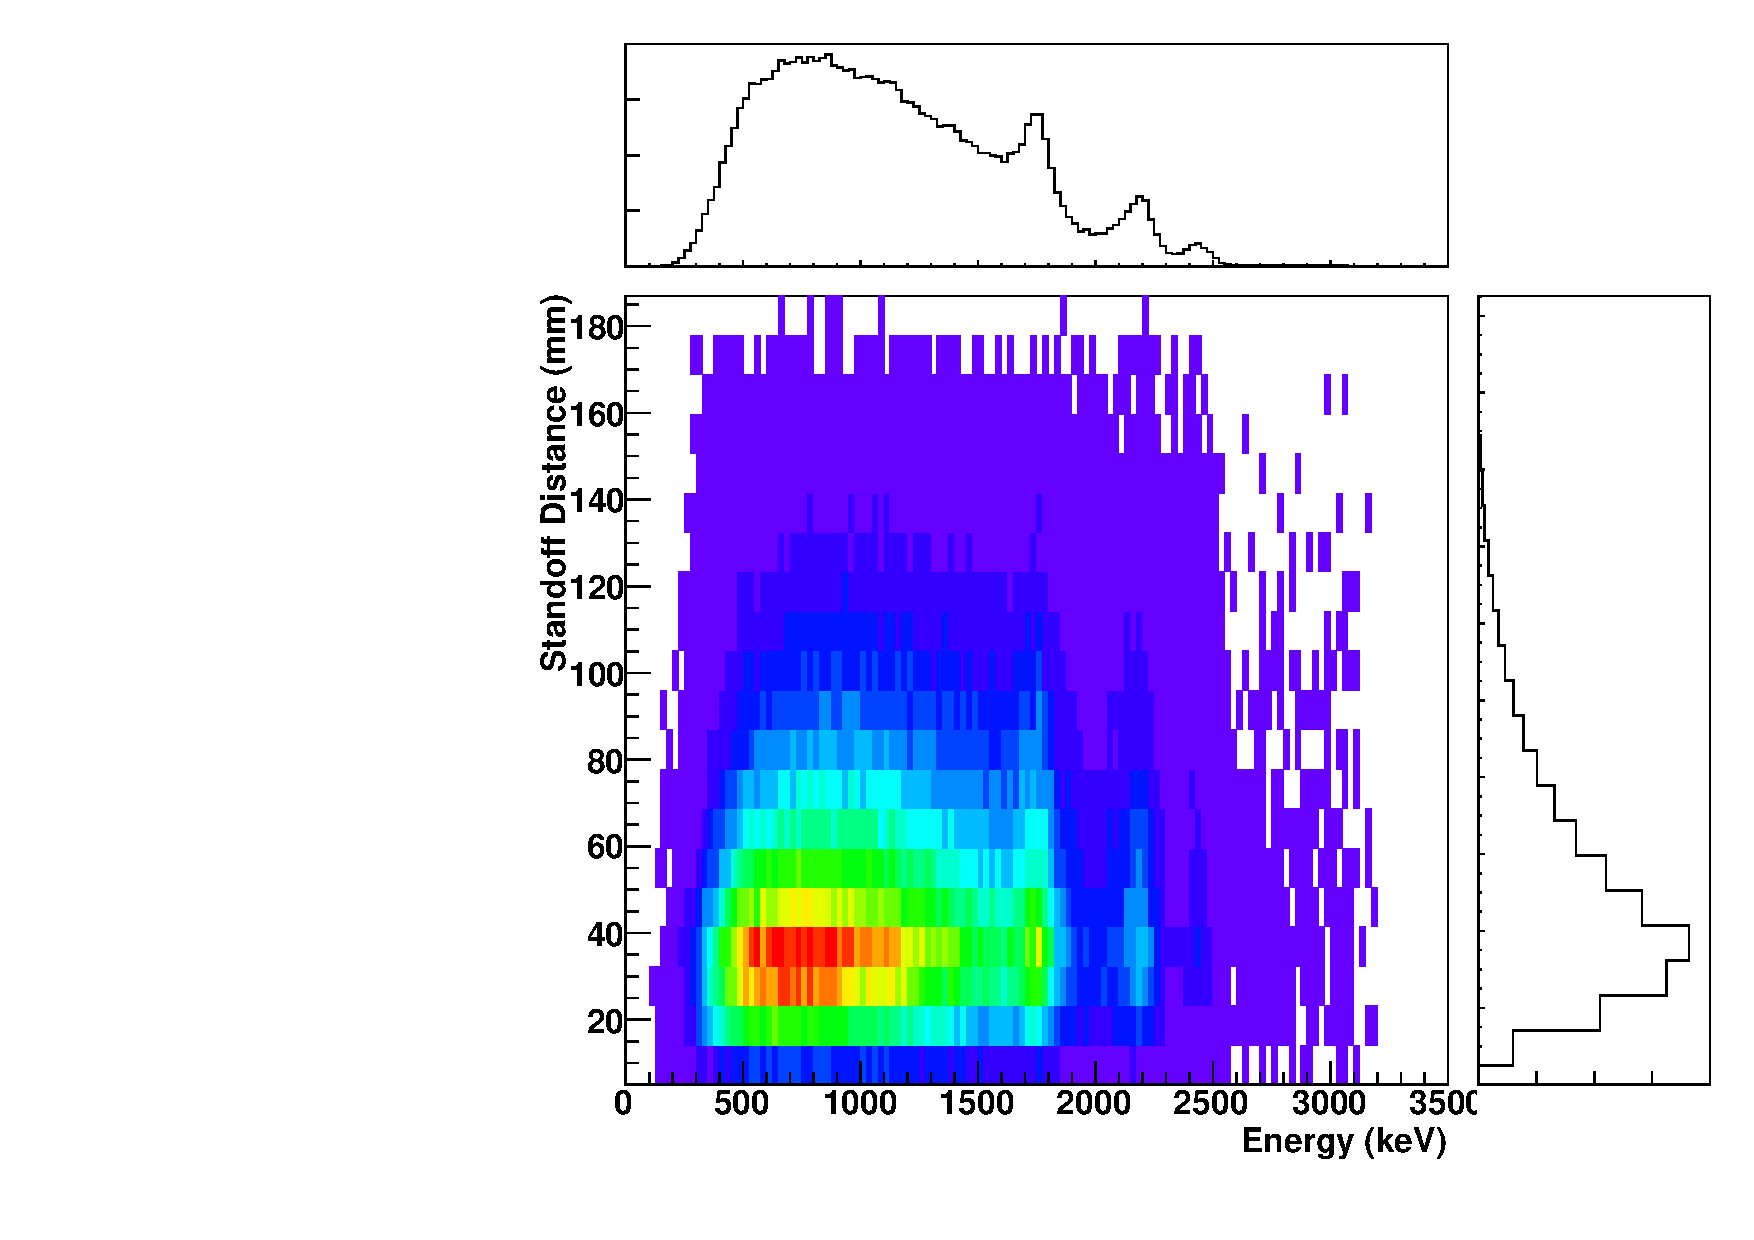
\includegraphics[width=1\textwidth]{./plots/PDFs/analysis_pdf_AirGap_214_Bi_nochain_ms.pdf}
	\end{subfigure}
\caption[PDF for \isotope{214}{Bi} in the airgap]{The two dimensional PDFs for \isotope{214}{Bi} in the airgap due to \isotope{222}{Rn}, with one-dimensional projections. Single site is shown on the left, and multiple site is shown on the right.}
\label{fig:analysis_pdf_AirGap_214_Bi_nochain}
\end{figure}

\end{document}